\usepackage{multirow}
\usepackage{wrapfig}
\usepackage{colortbl}
\usepackage{enumitem}

\setlist[itemize]{align=parleft,left=0pt}

\definecolor{realblue}{rgb}{0.3569, 0.6078, 0.8353}
\definecolor{synorange}{rgb}{0.9294, 0.4902, 0.1921}
\definecolor{azure(colorwheel)}{rgb}{0.0, 0.5, 1.0}
\definecolor{nicegreen}{rgb}{0.0, 0.7, 0.1}
\definecolor{CuGray}{gray}{0.9}
\definecolor{pink}{cmyk}{0, 0.7808, 0.4429, 0.1412}
\definecolor{amethyst}{rgb}{0.6, 0.4, 0.8}
\definecolor{black}{rgb}{0.0, 0.0, 0.0}


% \newcolumntype{w}{>{}c}
\newcolumntype{g}{>{\columncolor{CuGray}}c}
\newcolumntype{z}{>{\columncolor{CuGray}}l}

\renewcommand{\paragraph}[1]{\noindent\textbf{#1}\,\,}

\newcommand{\ck}[1]{\textcolor{blue}{#1}}
\newcommand{\sr}[1]{\textcolor{red}{#1}}
\newcommand{\oh}[1]{\textcolor{black}{#1}}
\newcommand{\moon}[1]{\textcolor{black}{#1}}
\newcommand{\nam}[1]{\textcolor{black}{#1}}
\newcommand{\nayeong}[1]{\textcolor{black}{#1}}
\newcommand{\wonseok}[1]{\textcolor{blue}{#1}}

\usepackage{xspace}

% \def\@onedot{\ifx\@let@token.\else.\null\fi\xspace}
% \DeclareRobustCommand\onedot{\futurelet\@let@token\@onedot}

\def\onedot{.\@\xspace}
\def\eg{\emph{e.g}\onedot} \def\Eg{{E.g}\onedot}
\def\ie{\emph{i.e}\onedot} \def\Ie{{I.e}\onedot}
\def\cf{\emph{c.f}\onedot} \def\Cf{{C.f}\onedot}
\def\etc{\emph{etc}\onedot} \def\vs{{vs}\onedot}
\def\wrt{\emph{w.r.t}\onedot} \def\dof{d.o.f\onedot}
\def\etal{\emph{et al}\onedot}



\newcommand{\Sref}[1]{Sec.~\ref{#1}}
\newcommand{\Eref}[1]{Eq.~(\ref{#1})}
\newcommand{\Fref}[1]{Fig.~\ref{#1}}
\newcommand{\Tref}[1]{Table~\ref{#1}}




\def\ours{$\mathbf{\mathtt{SYNAuG}}$}



% math bold for lower cases (a-z)
\newcommand{\ba}{{\mathbf{a}}}
\newcommand{\bb}{{\mathbf{b}}}
\newcommand{\bc}{{\mathbf{c}}}
\newcommand{\bd}{{\mathbf{d}}}
\newcommand{\bolde}{{\mathbf{e}}}
\newcommand{\boldf}{{\mathbf{f}}}
\newcommand{\bg}{{\mathbf{g}}}
\newcommand{\bh}{{\mathbf{h}}}
\newcommand{\bi}{{\mathbf{i}}}
\newcommand{\bj}{{\mathbf{j}}}
\newcommand{\bk}{{\mathbf{k}}}
\newcommand{\bl}{{\mathbf{l}}}
% \newcommand{\bm}{{\mathbf{m}}}
\newcommand{\bn}{{\mathbf{n}}}
\newcommand{\bo}{{\mathbf{o}}}
\newcommand{\bp}{{\mathbf{p}}}
\newcommand{\bq}{{\mathbf{q}}}
\newcommand{\br}{{\mathbf{r}}}
\newcommand{\bs}{{\mathbf{s}}}
\newcommand{\bt}{{\mathbf{t}}}
\newcommand{\bu}{{\mathbf{u}}}
\newcommand{\bv}{{\mathbf{v}}}
\newcommand{\bw}{{\mathbf{w}}}
\newcommand{\bx}{{\mathbf{x}}}
\newcommand{\by}{{\mathbf{y}}}
\newcommand{\bz}{{\mathbf{z}}}





% math bold for upper cases (A-Z)
\newcommand{\bA}{\mathbf{A}}
\newcommand{\bB}{\mathbf{B}}
\newcommand{\bC}{\mathbf{C}}
\newcommand{\bD}{\mathbf{D}}
\newcommand{\bE}{\mathbf{E}}
\newcommand{\bF}{\mathbf{F}}
\newcommand{\bG}{\mathbf{G}}
\newcommand{\bH}{\mathbf{H}}
\newcommand{\bI}{\mathbf{I}}
\newcommand{\bJ}{\mathbf{J}}
\newcommand{\bK}{\mathbf{K}}
\newcommand{\bL}{\mathbf{L}}
\newcommand{\bM}{\mathbf{M}}
\newcommand{\bN}{\mathbf{N}}
\newcommand{\bO}{\mathbf{O}}
\newcommand{\bP}{\mathbf{P}}
\newcommand{\bQ}{\mathbf{Q}}
\newcommand{\bR}{\mathbf{R}}
\newcommand{\bS}{\mathbf{S}}
\newcommand{\bT}{\mathbf{T}}
\newcommand{\bU}{\mathbf{U}}
\newcommand{\bV}{\mathbf{V}}
\newcommand{\bW}{\mathbf{W}}
\newcommand{\bX}{\mathbf{X}}
\newcommand{\bY}{\mathbf{Y}}
\newcommand{\bZ}{\mathbf{Z}}





% calligraphic
\newcommand{\calA}{{\mathcal{A}}}
\newcommand{\calB}{{\mathcal{B}}}
\newcommand{\calC}{{\mathcal{C}}}
\newcommand{\calD}{{\mathcal{D}}}
\newcommand{\calE}{{\mathcal{E}}}
\newcommand{\calF}{{\mathcal{F}}}
\newcommand{\calG}{{\mathcal{G}}}
\newcommand{\calH}{{\mathcal{H}}}
\newcommand{\calI}{{\mathcal{I}}}
\newcommand{\calJ}{{\mathcal{J}}}
\newcommand{\calK}{{\mathcal{K}}}
\newcommand{\calL}{{\mathcal{L}}}
\newcommand{\calM}{{\mathcal{M}}}
\newcommand{\calN}{{\mathcal{N}}}
\newcommand{\calO}{{\mathcal{O}}}
\newcommand{\calP}{{\mathcal{P}}}
\newcommand{\calQ}{{\mathcal{Q}}}
\newcommand{\calR}{{\mathcal{R}}}
\newcommand{\calS}{{\mathcal{S}}}
\newcommand{\calT}{{\mathcal{T}}}
\newcommand{\calU}{{\mathcal{U}}}
\newcommand{\calV}{{\mathcal{V}}}
\newcommand{\calW}{{\mathcal{W}}}
\newcommand{\calX}{{\mathcal{X}}}
\newcommand{\calY}{{\mathcal{Y}}}
\newcommand{\calZ}{{\mathcal{Z}}}
\newcommand{\calbX}{\mbox{\boldmath $\mathcal{X}$}}
\newcommand{\calbY}{\mbox{\boldmath $\mathcal{Y}$}}


\newcommand{\bcalA}{\mbox{\boldmath $\calA$}}
\newcommand{\bcalB}{\mbox{\boldmath $\calB$}}
\newcommand{\bcalC}{\mbox{\boldmath $\calC$}}
\newcommand{\bcalD}{\mbox{\boldmath $\calD$}}
\newcommand{\bcalE}{\mbox{\boldmath $\calE$}}
\newcommand{\bcalF}{\mbox{\boldmath $\calF$}}
\newcommand{\bcalG}{\mbox{\boldmath $\calG$}}
\newcommand{\bcalH}{\mbox{\boldmath $\calH$}}
\newcommand{\bcalI}{\mbox{\boldmath $\calI$}}
\newcommand{\bcalJ}{\mbox{\boldmath $\calJ$}}
\newcommand{\bcalK}{\mbox{\boldmath $\calK$}}
\newcommand{\bcalL}{\mbox{\boldmath $\calL$}}
\newcommand{\bcalM}{\mbox{\boldmath $\calM$}}
\newcommand{\bcalN}{\mbox{\boldmath $\calN$}}
\newcommand{\bcalO}{\mbox{\boldmath $\calO$}}
\newcommand{\bcalP}{\mbox{\boldmath $\calP$}}
\newcommand{\bcalQ}{\mbox{\boldmath $\calQ$}}
\newcommand{\bcalR}{\mbox{\boldmath $\calR$}}
\newcommand{\bcalS}{\mbox{\boldmath $\calS$}}
\newcommand{\bcalT}{\mbox{\boldmath $\calT$}}
\newcommand{\bcalU}{\mbox{\boldmath $\calU$}}
\newcommand{\bcalV}{\mbox{\boldmath $\calV$}}
\newcommand{\bcalW}{\mbox{\boldmath $\calW$}}
\newcommand{\bcalX}{\mbox{\boldmath $\calX$}}
\newcommand{\bcalY}{\mbox{\boldmath $\calY$}}
\newcommand{\bcalZ}{\mbox{\boldmath $\calZ$}}

\newcommand{\sfA}{\mbox{$\mathsf A$}}
\newcommand{\sfB}{\mbox{$\mathsf B$}}
\newcommand{\sfC}{\mbox{$\mathsf C$}}
\newcommand{\sfD}{\mbox{$\mathsf D$}}
\newcommand{\sfE}{\mbox{$\mathsf E$}}
\newcommand{\sfF}{\mbox{$\mathsf F$}}
\newcommand{\sfG}{\mbox{$\mathsf G$}}
\newcommand{\sfH}{\mbox{$\mathsf H$}}
\newcommand{\sfI}{\mbox{$\mathsf I$}}
\newcommand{\sfJ}{\mbox{$\mathsf J$}}
\newcommand{\sfK}{\mbox{$\mathsf K$}}
\newcommand{\sfL}{\mbox{$\mathsf L$}}
\newcommand{\sfM}{\mbox{$\mathsf M$}}
\newcommand{\sfN}{\mbox{$\mathsf N$}}
\newcommand{\sfO}{\mbox{$\mathsf O$}}
\newcommand{\sfP}{\mbox{$\mathsf P$}}
\newcommand{\sfQ}{\mbox{$\mathsf Q$}}
\newcommand{\sfR}{\mbox{$\mathsf R$}}
\newcommand{\sfS}{\mbox{$\mathsf S$}}
\newcommand{\sfT}{\mbox{$\mathsf T$}}
\newcommand{\sfU}{\mbox{$\mathsf U$}}
\newcommand{\sfV}{\mbox{$\mathsf V$}}
\newcommand{\sfW}{\mbox{$\mathsf W$}}
\newcommand{\sfX}{\mbox{$\mathsf X$}}
\newcommand{\sfY}{\mbox{$\mathsf Y$}}
\newcommand{\sfZ}{\mbox{$\mathsf Z$}}





% math bold for lower cases (Greek letters)
\newcommand{\balpha}{\mbox{\boldmath $\alpha$}}
\newcommand{\bbeta}{\mbox{\boldmath $\beta$}}
\newcommand{\bgamma}{\mbox{\boldmath $\gamma$}}
\newcommand{\bdelta}{\mbox{\boldmath $\delta$}}
\newcommand{\bepsilon}{\mbox{\boldmath $\epsilon$}}
\newcommand{\bvarepsilon}{\mbox{\boldmath $\varepsilon$}}
\newcommand{\bzeta}{\mbox{\boldmath $\zeta$}}
\newcommand{\boldeta}{\mbox{\boldmath $\eta$}}
\newcommand{\btheta}{\mbox{\boldmath $\theta$}}
\newcommand{\bvartheta}{\mbox{\boldmath $\vartheta$}}
\newcommand{\biota}{\mbox{\boldmath $\iota$}}
\newcommand{\bkappa}{\mbox{\boldmath $\kappa$}}
\newcommand{\blambda}{\mbox{\boldmath $\lambda$}}
\newcommand{\bmu}{\mbox{\boldmath $\mu$}}
\newcommand{\bnu}{\mbox{\boldmath $\nu$}}
\newcommand{\bxi}{\mbox{\boldmath $\xi$}}
\newcommand{\bpi}{\mbox{\boldmath $\pi$}}
\newcommand{\bvarpi}{\mbox{\boldmath $\varpi$}}
\newcommand{\brho}{\mbox{\boldmath $\rho$}}
\newcommand{\bvarrho}{\mbox{\boldmath $\varrho$}}
\newcommand{\bsigma}{\mbox{\boldmath $\sigma$}}
\newcommand{\bvarsigma}{\mbox{\boldmath $\varsigma$}}
\newcommand{\btau}{\mbox{\boldmath $\tau$}}
\newcommand{\bupsilon}{\mbox{\boldmath $\upsilon$}}
\newcommand{\bphi}{\mbox{\boldmath $\phi$}}
\newcommand{\bvarphi}{\mbox{\boldmath $\varphi$}}
\newcommand{\bchi}{\mbox{\boldmath $\chi$}}
\newcommand{\bpsi}{\mbox{\boldmath $\psi$}}
\newcommand{\bomega}{\mbox{\boldmath $\omega$}}





% math bold for upper cases (Greek Letters)
\newcommand{\bGamma}{\mbox{\boldmath $\Gamma$}}
\newcommand{\bDelta}{\mbox{\boldmath $\Delta$}}
\newcommand{\bTheta}{\mbox{\boldmath $\Theta$}}
\newcommand{\bLambda}{\mbox{\boldmath $\Lambda$}}
\newcommand{\bXi}{\mbox{\boldmath $\Xi$}}
\newcommand{\bPi}{\mbox{\boldmath $\Pi$}}
\newcommand{\bSigma}{\mbox{\boldmath $\Sigma$}}
\newcommand{\bUpsilon}{\mbox{\boldmath $\Upsilon$}}
\newcommand{\bPhi}{\mbox{\boldmath $\Phi$}}
\newcommand{\bPsi}{\mbox{\boldmath $\Psi$}}
\newcommand{\bOmega}{\mbox{\boldmath $\Omega$}}





% vector notation for lower cases (a-z)
\newcommand{\veca}{{\vec{\ba}}}
\newcommand{\vecb}{{\vec{\bb}}}
\newcommand{\vecc}{{\vec{\bc}}}
\newcommand{\vecd}{{\vec{\bd}}}
\newcommand{\vece}{{\vec{\bolde}}}
\newcommand{\vecf}{{\vec{\boldf}}}
\newcommand{\vecg}{{\vec{\bg}}}
\newcommand{\vech}{{\vec{\bh}}}
\newcommand{\veci}{{\vec{\bi}}}
\newcommand{\vecj}{{\vec{\bj}}}
\newcommand{\veck}{{\vec{\bk}}}
\newcommand{\vecl}{{\vec{\bl}}}
\newcommand{\vecm}{{\vec{\bm}}}
\newcommand{\vecn}{{\vec{\bn}}}
\newcommand{\veco}{{\vec{\bo}}}
\newcommand{\vecp}{{\vec{\bp}}}
\newcommand{\vecq}{{\vec{\bq}}}
\newcommand{\vecr}{{\vec{\br}}}
\newcommand{\vecs}{{\vec{\bs}}}
\newcommand{\vect}{{\vec{\bt}}}
\newcommand{\vecu}{{\vec{\bu}}}
\newcommand{\vecv}{{\vec{\bv}}}
\newcommand{\vecw}{{\vec{\bw}}}
\newcommand{\vecx}{{\vec{\bx}}}
\newcommand{\vecy}{{\vec{\by}}}
\newcommand{\vecz}{{\vec{\bz}}}

\newcommand{\vecxi}{{\vec{\bxi}}}
\newcommand{\vecphi}{{\vec{\bphi}}}
\newcommand{\vecvarphi}{{\vec{\bvarphi}}}
\newcommand{\vecbeta}{{\vec{\bbeta}}}
\newcommand{\vecdelta}{{\vec{\bdelta}}}
\newcommand{\vectheta}{{\vec{\btheta}}}


% set of numbers
\newcommand{\Real}{\mathbb R}
\newcommand{\Complex}{\mathbb C}
\newcommand{\Natural}{\mathbb N}
\newcommand{\Integer}{\mathbb Z}



% ets
\newcommand{\bone}{\mbox{\boldmath $1$}}
\newcommand{\bzero}{\mbox{\boldmath $0$}}
\newcommand{\0}{{\bf 0}}

\newcommand{\be}{\begin{eqnarray}}
\newcommand{\ee}{\end{eqnarray}}
\newcommand{\bee}{\begin{eqnarray*}}
\newcommand{\eee}{\end{eqnarray*}}

\newcommand{\matrixb}{\left[ \begin{array}}
\newcommand{\matrixe}{\end{array} \right]}   

\newtheorem{theorem}{{Theorem}}
\newtheorem{lemma}{{Lemma}}
\newtheorem{corollary}{{Corollary}}
\newtheorem{definition}{{Definition}}
\newtheorem{proposition}{{Proposition}}
\newtheorem{remark}{{Remark}}
\newtheorem{example}{{Example}}
%\newtheorem{algorithm}{{Algorithm}}

\newcommand{\argmax}{\operatornamewithlimits{\arg \max}}
\newcommand{\argmin}{\operatornamewithlimits{\arg \min}}

\newcommand{\mean}[1]{\left \langle #1 \right \rangle}
\newcommand{\ave}{\mathbb E}
\newcommand{\E}{\mathbb E}
\newcommand{\empha}[1]{{\color{red} \bf #1}}
\newcommand{\fracpartial}[2]{\frac{\partial #1}{\partial  #2}}
\newcommand{\incomplete}[1]{\textcolor{red}{#1}}



\def\doublespace{\renewcommand{\baselinestretch}{2}\large\normalsize}
\def\singlespace{\renewcommand{\baselinestretch}{1}\large\normalsize}
\def\onehalfspace{\renewcommand{\baselinestretch}{1.5}\large\normalsize}
\def\onequaterspace{\renewcommand{\baselinestretch}{1.3}\large\normalsize}
\def\threequaterspace{\renewcommand{\baselinestretch}{1.7}\large\normalsize}
\def\smallspace{\renewcommand{\baselinestretch}{-.9}\large\normalsize}
\def\tinyspace{\renewcommand{\baselinestretch}{-.7}\large\normalsize}

\newcommand{\tr} { \textrm{tr} }
\newcommand{\re} { \textrm{re} }
\newcommand{\im} { \textrm{im} }
\newcommand{\diag} { \textrm{diag} }
\newcommand{\ddiag} { \textrm{ddiag} }
\newcommand{\off} { \textrm{off} }
\newcommand{\vectxt} { \textrm{vec} }

\newcommand{\lla}{\left\langle}
\newcommand{\rra}{\right\rangle}
\newcommand{\llbr}{\left\lbrack}
\newcommand{\rrbr}{\right\rbrack}
\newcommand{\llb}{\left\lbrace}
\newcommand{\rrb}{\right\rbrace}

\begin{table}[t]
\centering
\caption{CIFAR100-LT, ResNet32, ablation in terms of the number of additional data
}
\resizebox{0.7\linewidth}{!}{
    \begin{tabular}{@{}lcccccc}
        \toprule
        \multirow{2}[2]{*}{\textbf{{Method}}} & \multicolumn{4}{c}{\textbf{IF=100}} & \multirow{2}[2]{*}{\textbf{{50}}} & \multirow{2}[2]{*}{\textbf{{10}}} \\
        \cmidrule{2-5}
        & \textbf{Many} & \textbf{Medium} & \textbf{Few} & \textbf{All} & & \\        
        \midrule
        LT                      & 68.31 & 36.88 & 4.87 & 37.96 & 43.54 & 59.50 \\
        \cmidrule{1-7}
        Uniform (250)           & 69.69 & 51.35 & 27.55 & 50.39 & 54.42 & 62.74 \\
        LT + 250                & 74.74 & 50.88 & 28.55 & 52.31 & 55.76 & 66.02 \\
        Uniform (500)           & 75.23 & 52.15 & 30.58 & 53.54 & 57.09 & 66.66 \\
        LT + 500                & 75.74 & 52.27 & 30.77 & 53.82 & 57.63 & 67.62 \\
        Uniform (1k)            & 75.94 & 54.91 & 33.16 & 55.53 & 59.38 & 68.59 \\
        \bottomrule 
    \end{tabular}
    }
    \label{tab:cifar100_lt_abl}
\end{table}






\paragraph{Detail Settings of Figure 1.}
We conduct toy experiments to validate our argument.
We sample training data from the normal distributions, $\calN(\bm{\mu}_{ca}, \bm{\sigma})$, where $\bm{\mu}_{00}, \bm{\mu}_{01}, \bm{\mu}_{10}, \bm{\mu}_{11} \in \Real^{2}$ are the means vectors, $c$ is the class, $a$ is the sensitive attribute, and $\bm{\sigma} \in \Real^{2\times 2}$ is the covariance matrix.
We train the 2-layer neural network on these samples and plot the learned classifier.
We visualize the learned classifier in \Fref{fig:fair_toy}.
When both class imbalance and sensitive attributed are imbalanced, the learned classifier is far from the fair classifier, which is vertical.
The next unfair classifier happens when the class imbalance exists.
In conclusion, mitigating the class imbalance is essential as the long-tail distribution.
% WACV 2024 Paper Template
% based on the CVPR 2023 template (https://media.icml.cc/Conferences/CVPR2023/cvpr2023-author_kit-v1_1-1.zip) with 2-track changes from the WACV 2023 template (https://github.com/wacv-pcs/WACV-2023-Author-Kit)
% based on the CVPR template provided by Ming-Ming Cheng (https://github.com/MCG-NKU/CVPR_Template)
% modified and extended by Stefan Roth (stefan.roth@NOSPAMtu-darmstadt.de)

\documentclass[10pt,twocolumn,letterpaper]{article}

%%%%%%%%% PAPER TYPE  - PLEASE UPDATE FOR FINAL VERSION
% \usepackage[review,algorithms]{wacv}      % To produce the REVIEW version for the algorithms track
%\usepackage[review,applications]{wacv}      % To produce the REVIEW version for the applications track
\usepackage{wacv}              % To produce the CAMERA-READY version
%\usepackage[pagenumbers]{wacv} % To force page numbers, e.g. for an arXiv version

% Include other packages here, before hyperref.
\usepackage{graphicx}
\usepackage{amsmath}
\usepackage{amssymb}
\usepackage{booktabs}
\usepackage{makecell}


% It is strongly recommended to use hyperref, especially for the review version.
% hyperref with option pagebackref eases the reviewers' job.
% Please disable hyperref *only* if you encounter grave issues, e.g. with the
% file validation for the camera-ready version.
%
% If you comment hyperref and then uncomment it, you should delete
% ReviewTempalte.aux before re-running LaTeX.
% (Or just hit 'q' on the first LaTeX run, let it finish, and you
%  should be clear).
\usepackage[pagebackref,breaklinks,colorlinks]{hyperref}


% Support for easy cross-referencing
\usepackage[capitalize]{cleveref}
\crefname{section}{Sec.}{Secs.}
\Crefname{section}{Section}{Sections}
\Crefname{table}{Table}{Tables}
\crefname{table}{Tab.}{Tabs.}


%%%%%%%%% PAPER ID  - PLEASE UPDATE
\def\wacvPaperID{1347} % *** Enter the WACV Paper ID here
\def\confName{WACV}
\def\confYear{2024}

\usepackage{multirow}
\usepackage{wrapfig}
\usepackage{colortbl}
\usepackage{enumitem}

\setlist[itemize]{align=parleft,left=0pt}

\definecolor{realblue}{rgb}{0.3569, 0.6078, 0.8353}
\definecolor{synorange}{rgb}{0.9294, 0.4902, 0.1921}
\definecolor{azure(colorwheel)}{rgb}{0.0, 0.5, 1.0}
\definecolor{nicegreen}{rgb}{0.0, 0.7, 0.1}
\definecolor{CuGray}{gray}{0.9}
\definecolor{pink}{cmyk}{0, 0.7808, 0.4429, 0.1412}
\definecolor{amethyst}{rgb}{0.6, 0.4, 0.8}
\definecolor{black}{rgb}{0.0, 0.0, 0.0}


% \newcolumntype{w}{>{}c}
\newcolumntype{g}{>{\columncolor{CuGray}}c}
\newcolumntype{z}{>{\columncolor{CuGray}}l}

\renewcommand{\paragraph}[1]{\noindent\textbf{#1}\,\,}

\newcommand{\ck}[1]{\textcolor{blue}{#1}}
\newcommand{\sr}[1]{\textcolor{red}{#1}}
\newcommand{\oh}[1]{\textcolor{black}{#1}}
\newcommand{\moon}[1]{\textcolor{black}{#1}}
\newcommand{\nam}[1]{\textcolor{black}{#1}}
\newcommand{\nayeong}[1]{\textcolor{black}{#1}}
\newcommand{\wonseok}[1]{\textcolor{blue}{#1}}

\usepackage{xspace}

% \def\@onedot{\ifx\@let@token.\else.\null\fi\xspace}
% \DeclareRobustCommand\onedot{\futurelet\@let@token\@onedot}

\def\onedot{.\@\xspace}
\def\eg{\emph{e.g}\onedot} \def\Eg{{E.g}\onedot}
\def\ie{\emph{i.e}\onedot} \def\Ie{{I.e}\onedot}
\def\cf{\emph{c.f}\onedot} \def\Cf{{C.f}\onedot}
\def\etc{\emph{etc}\onedot} \def\vs{{vs}\onedot}
\def\wrt{\emph{w.r.t}\onedot} \def\dof{d.o.f\onedot}
\def\etal{\emph{et al}\onedot}



\newcommand{\Sref}[1]{Sec.~\ref{#1}}
\newcommand{\Eref}[1]{Eq.~(\ref{#1})}
\newcommand{\Fref}[1]{Fig.~\ref{#1}}
\newcommand{\Tref}[1]{Table~\ref{#1}}




\def\ours{$\mathbf{\mathtt{SYNAuG}}$}



% math bold for lower cases (a-z)
\newcommand{\ba}{{\mathbf{a}}}
\newcommand{\bb}{{\mathbf{b}}}
\newcommand{\bc}{{\mathbf{c}}}
\newcommand{\bd}{{\mathbf{d}}}
\newcommand{\bolde}{{\mathbf{e}}}
\newcommand{\boldf}{{\mathbf{f}}}
\newcommand{\bg}{{\mathbf{g}}}
\newcommand{\bh}{{\mathbf{h}}}
\newcommand{\bi}{{\mathbf{i}}}
\newcommand{\bj}{{\mathbf{j}}}
\newcommand{\bk}{{\mathbf{k}}}
\newcommand{\bl}{{\mathbf{l}}}
% \newcommand{\bm}{{\mathbf{m}}}
\newcommand{\bn}{{\mathbf{n}}}
\newcommand{\bo}{{\mathbf{o}}}
\newcommand{\bp}{{\mathbf{p}}}
\newcommand{\bq}{{\mathbf{q}}}
\newcommand{\br}{{\mathbf{r}}}
\newcommand{\bs}{{\mathbf{s}}}
\newcommand{\bt}{{\mathbf{t}}}
\newcommand{\bu}{{\mathbf{u}}}
\newcommand{\bv}{{\mathbf{v}}}
\newcommand{\bw}{{\mathbf{w}}}
\newcommand{\bx}{{\mathbf{x}}}
\newcommand{\by}{{\mathbf{y}}}
\newcommand{\bz}{{\mathbf{z}}}





% math bold for upper cases (A-Z)
\newcommand{\bA}{\mathbf{A}}
\newcommand{\bB}{\mathbf{B}}
\newcommand{\bC}{\mathbf{C}}
\newcommand{\bD}{\mathbf{D}}
\newcommand{\bE}{\mathbf{E}}
\newcommand{\bF}{\mathbf{F}}
\newcommand{\bG}{\mathbf{G}}
\newcommand{\bH}{\mathbf{H}}
\newcommand{\bI}{\mathbf{I}}
\newcommand{\bJ}{\mathbf{J}}
\newcommand{\bK}{\mathbf{K}}
\newcommand{\bL}{\mathbf{L}}
\newcommand{\bM}{\mathbf{M}}
\newcommand{\bN}{\mathbf{N}}
\newcommand{\bO}{\mathbf{O}}
\newcommand{\bP}{\mathbf{P}}
\newcommand{\bQ}{\mathbf{Q}}
\newcommand{\bR}{\mathbf{R}}
\newcommand{\bS}{\mathbf{S}}
\newcommand{\bT}{\mathbf{T}}
\newcommand{\bU}{\mathbf{U}}
\newcommand{\bV}{\mathbf{V}}
\newcommand{\bW}{\mathbf{W}}
\newcommand{\bX}{\mathbf{X}}
\newcommand{\bY}{\mathbf{Y}}
\newcommand{\bZ}{\mathbf{Z}}





% calligraphic
\newcommand{\calA}{{\mathcal{A}}}
\newcommand{\calB}{{\mathcal{B}}}
\newcommand{\calC}{{\mathcal{C}}}
\newcommand{\calD}{{\mathcal{D}}}
\newcommand{\calE}{{\mathcal{E}}}
\newcommand{\calF}{{\mathcal{F}}}
\newcommand{\calG}{{\mathcal{G}}}
\newcommand{\calH}{{\mathcal{H}}}
\newcommand{\calI}{{\mathcal{I}}}
\newcommand{\calJ}{{\mathcal{J}}}
\newcommand{\calK}{{\mathcal{K}}}
\newcommand{\calL}{{\mathcal{L}}}
\newcommand{\calM}{{\mathcal{M}}}
\newcommand{\calN}{{\mathcal{N}}}
\newcommand{\calO}{{\mathcal{O}}}
\newcommand{\calP}{{\mathcal{P}}}
\newcommand{\calQ}{{\mathcal{Q}}}
\newcommand{\calR}{{\mathcal{R}}}
\newcommand{\calS}{{\mathcal{S}}}
\newcommand{\calT}{{\mathcal{T}}}
\newcommand{\calU}{{\mathcal{U}}}
\newcommand{\calV}{{\mathcal{V}}}
\newcommand{\calW}{{\mathcal{W}}}
\newcommand{\calX}{{\mathcal{X}}}
\newcommand{\calY}{{\mathcal{Y}}}
\newcommand{\calZ}{{\mathcal{Z}}}
\newcommand{\calbX}{\mbox{\boldmath $\mathcal{X}$}}
\newcommand{\calbY}{\mbox{\boldmath $\mathcal{Y}$}}


\newcommand{\bcalA}{\mbox{\boldmath $\calA$}}
\newcommand{\bcalB}{\mbox{\boldmath $\calB$}}
\newcommand{\bcalC}{\mbox{\boldmath $\calC$}}
\newcommand{\bcalD}{\mbox{\boldmath $\calD$}}
\newcommand{\bcalE}{\mbox{\boldmath $\calE$}}
\newcommand{\bcalF}{\mbox{\boldmath $\calF$}}
\newcommand{\bcalG}{\mbox{\boldmath $\calG$}}
\newcommand{\bcalH}{\mbox{\boldmath $\calH$}}
\newcommand{\bcalI}{\mbox{\boldmath $\calI$}}
\newcommand{\bcalJ}{\mbox{\boldmath $\calJ$}}
\newcommand{\bcalK}{\mbox{\boldmath $\calK$}}
\newcommand{\bcalL}{\mbox{\boldmath $\calL$}}
\newcommand{\bcalM}{\mbox{\boldmath $\calM$}}
\newcommand{\bcalN}{\mbox{\boldmath $\calN$}}
\newcommand{\bcalO}{\mbox{\boldmath $\calO$}}
\newcommand{\bcalP}{\mbox{\boldmath $\calP$}}
\newcommand{\bcalQ}{\mbox{\boldmath $\calQ$}}
\newcommand{\bcalR}{\mbox{\boldmath $\calR$}}
\newcommand{\bcalS}{\mbox{\boldmath $\calS$}}
\newcommand{\bcalT}{\mbox{\boldmath $\calT$}}
\newcommand{\bcalU}{\mbox{\boldmath $\calU$}}
\newcommand{\bcalV}{\mbox{\boldmath $\calV$}}
\newcommand{\bcalW}{\mbox{\boldmath $\calW$}}
\newcommand{\bcalX}{\mbox{\boldmath $\calX$}}
\newcommand{\bcalY}{\mbox{\boldmath $\calY$}}
\newcommand{\bcalZ}{\mbox{\boldmath $\calZ$}}

\newcommand{\sfA}{\mbox{$\mathsf A$}}
\newcommand{\sfB}{\mbox{$\mathsf B$}}
\newcommand{\sfC}{\mbox{$\mathsf C$}}
\newcommand{\sfD}{\mbox{$\mathsf D$}}
\newcommand{\sfE}{\mbox{$\mathsf E$}}
\newcommand{\sfF}{\mbox{$\mathsf F$}}
\newcommand{\sfG}{\mbox{$\mathsf G$}}
\newcommand{\sfH}{\mbox{$\mathsf H$}}
\newcommand{\sfI}{\mbox{$\mathsf I$}}
\newcommand{\sfJ}{\mbox{$\mathsf J$}}
\newcommand{\sfK}{\mbox{$\mathsf K$}}
\newcommand{\sfL}{\mbox{$\mathsf L$}}
\newcommand{\sfM}{\mbox{$\mathsf M$}}
\newcommand{\sfN}{\mbox{$\mathsf N$}}
\newcommand{\sfO}{\mbox{$\mathsf O$}}
\newcommand{\sfP}{\mbox{$\mathsf P$}}
\newcommand{\sfQ}{\mbox{$\mathsf Q$}}
\newcommand{\sfR}{\mbox{$\mathsf R$}}
\newcommand{\sfS}{\mbox{$\mathsf S$}}
\newcommand{\sfT}{\mbox{$\mathsf T$}}
\newcommand{\sfU}{\mbox{$\mathsf U$}}
\newcommand{\sfV}{\mbox{$\mathsf V$}}
\newcommand{\sfW}{\mbox{$\mathsf W$}}
\newcommand{\sfX}{\mbox{$\mathsf X$}}
\newcommand{\sfY}{\mbox{$\mathsf Y$}}
\newcommand{\sfZ}{\mbox{$\mathsf Z$}}





% math bold for lower cases (Greek letters)
\newcommand{\balpha}{\mbox{\boldmath $\alpha$}}
\newcommand{\bbeta}{\mbox{\boldmath $\beta$}}
\newcommand{\bgamma}{\mbox{\boldmath $\gamma$}}
\newcommand{\bdelta}{\mbox{\boldmath $\delta$}}
\newcommand{\bepsilon}{\mbox{\boldmath $\epsilon$}}
\newcommand{\bvarepsilon}{\mbox{\boldmath $\varepsilon$}}
\newcommand{\bzeta}{\mbox{\boldmath $\zeta$}}
\newcommand{\boldeta}{\mbox{\boldmath $\eta$}}
\newcommand{\btheta}{\mbox{\boldmath $\theta$}}
\newcommand{\bvartheta}{\mbox{\boldmath $\vartheta$}}
\newcommand{\biota}{\mbox{\boldmath $\iota$}}
\newcommand{\bkappa}{\mbox{\boldmath $\kappa$}}
\newcommand{\blambda}{\mbox{\boldmath $\lambda$}}
\newcommand{\bmu}{\mbox{\boldmath $\mu$}}
\newcommand{\bnu}{\mbox{\boldmath $\nu$}}
\newcommand{\bxi}{\mbox{\boldmath $\xi$}}
\newcommand{\bpi}{\mbox{\boldmath $\pi$}}
\newcommand{\bvarpi}{\mbox{\boldmath $\varpi$}}
\newcommand{\brho}{\mbox{\boldmath $\rho$}}
\newcommand{\bvarrho}{\mbox{\boldmath $\varrho$}}
\newcommand{\bsigma}{\mbox{\boldmath $\sigma$}}
\newcommand{\bvarsigma}{\mbox{\boldmath $\varsigma$}}
\newcommand{\btau}{\mbox{\boldmath $\tau$}}
\newcommand{\bupsilon}{\mbox{\boldmath $\upsilon$}}
\newcommand{\bphi}{\mbox{\boldmath $\phi$}}
\newcommand{\bvarphi}{\mbox{\boldmath $\varphi$}}
\newcommand{\bchi}{\mbox{\boldmath $\chi$}}
\newcommand{\bpsi}{\mbox{\boldmath $\psi$}}
\newcommand{\bomega}{\mbox{\boldmath $\omega$}}





% math bold for upper cases (Greek Letters)
\newcommand{\bGamma}{\mbox{\boldmath $\Gamma$}}
\newcommand{\bDelta}{\mbox{\boldmath $\Delta$}}
\newcommand{\bTheta}{\mbox{\boldmath $\Theta$}}
\newcommand{\bLambda}{\mbox{\boldmath $\Lambda$}}
\newcommand{\bXi}{\mbox{\boldmath $\Xi$}}
\newcommand{\bPi}{\mbox{\boldmath $\Pi$}}
\newcommand{\bSigma}{\mbox{\boldmath $\Sigma$}}
\newcommand{\bUpsilon}{\mbox{\boldmath $\Upsilon$}}
\newcommand{\bPhi}{\mbox{\boldmath $\Phi$}}
\newcommand{\bPsi}{\mbox{\boldmath $\Psi$}}
\newcommand{\bOmega}{\mbox{\boldmath $\Omega$}}





% vector notation for lower cases (a-z)
\newcommand{\veca}{{\vec{\ba}}}
\newcommand{\vecb}{{\vec{\bb}}}
\newcommand{\vecc}{{\vec{\bc}}}
\newcommand{\vecd}{{\vec{\bd}}}
\newcommand{\vece}{{\vec{\bolde}}}
\newcommand{\vecf}{{\vec{\boldf}}}
\newcommand{\vecg}{{\vec{\bg}}}
\newcommand{\vech}{{\vec{\bh}}}
\newcommand{\veci}{{\vec{\bi}}}
\newcommand{\vecj}{{\vec{\bj}}}
\newcommand{\veck}{{\vec{\bk}}}
\newcommand{\vecl}{{\vec{\bl}}}
\newcommand{\vecm}{{\vec{\bm}}}
\newcommand{\vecn}{{\vec{\bn}}}
\newcommand{\veco}{{\vec{\bo}}}
\newcommand{\vecp}{{\vec{\bp}}}
\newcommand{\vecq}{{\vec{\bq}}}
\newcommand{\vecr}{{\vec{\br}}}
\newcommand{\vecs}{{\vec{\bs}}}
\newcommand{\vect}{{\vec{\bt}}}
\newcommand{\vecu}{{\vec{\bu}}}
\newcommand{\vecv}{{\vec{\bv}}}
\newcommand{\vecw}{{\vec{\bw}}}
\newcommand{\vecx}{{\vec{\bx}}}
\newcommand{\vecy}{{\vec{\by}}}
\newcommand{\vecz}{{\vec{\bz}}}

\newcommand{\vecxi}{{\vec{\bxi}}}
\newcommand{\vecphi}{{\vec{\bphi}}}
\newcommand{\vecvarphi}{{\vec{\bvarphi}}}
\newcommand{\vecbeta}{{\vec{\bbeta}}}
\newcommand{\vecdelta}{{\vec{\bdelta}}}
\newcommand{\vectheta}{{\vec{\btheta}}}


% set of numbers
\newcommand{\Real}{\mathbb R}
\newcommand{\Complex}{\mathbb C}
\newcommand{\Natural}{\mathbb N}
\newcommand{\Integer}{\mathbb Z}



% ets
\newcommand{\bone}{\mbox{\boldmath $1$}}
\newcommand{\bzero}{\mbox{\boldmath $0$}}
\newcommand{\0}{{\bf 0}}

\newcommand{\be}{\begin{eqnarray}}
\newcommand{\ee}{\end{eqnarray}}
\newcommand{\bee}{\begin{eqnarray*}}
\newcommand{\eee}{\end{eqnarray*}}

\newcommand{\matrixb}{\left[ \begin{array}}
\newcommand{\matrixe}{\end{array} \right]}   

\newtheorem{theorem}{{Theorem}}
\newtheorem{lemma}{{Lemma}}
\newtheorem{corollary}{{Corollary}}
\newtheorem{definition}{{Definition}}
\newtheorem{proposition}{{Proposition}}
\newtheorem{remark}{{Remark}}
\newtheorem{example}{{Example}}
%\newtheorem{algorithm}{{Algorithm}}

\newcommand{\argmax}{\operatornamewithlimits{\arg \max}}
\newcommand{\argmin}{\operatornamewithlimits{\arg \min}}

\newcommand{\mean}[1]{\left \langle #1 \right \rangle}
\newcommand{\ave}{\mathbb E}
\newcommand{\E}{\mathbb E}
\newcommand{\empha}[1]{{\color{red} \bf #1}}
\newcommand{\fracpartial}[2]{\frac{\partial #1}{\partial  #2}}
\newcommand{\incomplete}[1]{\textcolor{red}{#1}}



\def\doublespace{\renewcommand{\baselinestretch}{2}\large\normalsize}
\def\singlespace{\renewcommand{\baselinestretch}{1}\large\normalsize}
\def\onehalfspace{\renewcommand{\baselinestretch}{1.5}\large\normalsize}
\def\onequaterspace{\renewcommand{\baselinestretch}{1.3}\large\normalsize}
\def\threequaterspace{\renewcommand{\baselinestretch}{1.7}\large\normalsize}
\def\smallspace{\renewcommand{\baselinestretch}{-.9}\large\normalsize}
\def\tinyspace{\renewcommand{\baselinestretch}{-.7}\large\normalsize}

\newcommand{\tr} { \textrm{tr} }
\newcommand{\re} { \textrm{re} }
\newcommand{\im} { \textrm{im} }
\newcommand{\diag} { \textrm{diag} }
\newcommand{\ddiag} { \textrm{ddiag} }
\newcommand{\off} { \textrm{off} }
\newcommand{\vectxt} { \textrm{vec} }

\newcommand{\lla}{\left\langle}
\newcommand{\rra}{\right\rangle}
\newcommand{\llbr}{\left\lbrack}
\newcommand{\rrbr}{\right\rbrack}
\newcommand{\llb}{\left\lbrace}
\newcommand{\rrb}{\right\rbrace}

\begin{document}

%%%%%%%%% TITLE - PLEASE UPDATE
\title{SYNAuG: Exploiting Synthetic Data for Data Imbalance Problems}

\author{
\begin{tabular}{c c c c}
     & Moon Ye-Bin${}^{1}$\thanks{Authors contributed equally to this work.} & Nam Hyeon-Woo${}^{1}$\footnotemark[1] &  \\
    Wonseok Choi${}^{1}$ & Nayeong Kim${}^{1}$ & Suha Kwak${}^{1}$ & Tae-Hyun Oh${}^{1,2}$ \vspace{2mm}\\
\end{tabular}\\
    ${}^{1}$POSTECH, \quad${}^{2}$Yonsei University\\
    % ${}^{1}$Dept.~of Electrical Engineering and ${}^{2}$Grad.~School of Artificial Intelligence, POSTECH \\
    % ${}^{3}$Dept.~of  Computer Science and Engineering, POSTECH \\
    % ${}^{4}$Institute for Convergence Research and Education in Advanced Technology, Yonsei University\vspace{1mm}\\
    \texttt{\footnotesize{\{ybmoon, hyeonw.nam, wonseok.c, nayeong.kim, suha.kwak, taehyun\}@postech.ac.kr}}
}
\maketitle

%%%%%%%%% ABSTRACT
\begin{abstract}
    Entity alignment, aiming to identify equivalent entities across different knowledge graphs (KGs), is a fundamental problem for constructing Web-scale KGs. 
Over the course of its development, the label supervision has been considered necessary for accurate alignments. 
Inspired by the recent progress of self-supervised learning, we explore the extent to which we can get rid of supervision for entity alignment. 
Commonly, the label information (positive entity pairs) is used to supervise the process of pulling the aligned entities in each positive pair closer.
However, our theoretical analysis suggests that the learning of entity alignment can actually benefit more from 
pushing unlabeled negative pairs far away from each other than pulling labeled positive pairs close. 
%pushing unlabeled entities in sampled negative pairs far away than pulling those in positive pairs close.}
By leveraging this discovery, we develop the self-supervised learning objective for entity alignment.
We present \solution with efficient strategies to optimize this \hhy{objective} for aligning entities without label supervision. 
Extensive experiments on benchmark datasets demonstrate that \solution~without supervision can 
match or achieve comparable results with state-of-the-art supervised baselines. 
The performance of \solution suggests that self-supervised learning offers great potential for entity alignment in KGs. 
{The code and data are available at \url{https://github.com/THUDM/SelfKG}}.
\end{abstract}


%%%%%%%%% BODY TEXT
\section{Introduction}\label{sec:intro}

Deep neural networks (DNNs) have achieved strong performance on visual tasks.
The outstanding performance has been demonstrated by training a model with abundant and diverse labeled data
% ,~\eg,
~\cite{deng2009imagenet, lin2014microsoft}.
Despite the importance of data, machine learning researchers have focused mainly on the model and algorithms~\cite{sambasivan2021everyone}.
We should care about the data for training DNNs because unexpected influences can occur by data.
% and there is a lack of data debugging tools.
% We should first curate the dataset well for training the model because unexpected cascades can occur depending on the curated data~\cite{sambasivan2021everyone}.
% However, such abundant and well-curated labeled data are not available.
% The state-of-the-art DNNs suffer from much lower performance in certain types of classes or groups because of data imbalance.

We commonly encounter data imbalance problems categorized into \emph{class} or \emph{group} imbalance problems.
% The data imbalance problems we commonly encounter are mainly categorized into \emph{class} or \emph{group} imbalance problems.
Class imbalance means different data amounts in the classes.
Suppose that we collect animal images on the internet.
Images of rare animals may be found on search engines less than cats or dogs because of human bias for uploading their photograph~\footnote{For example, the number of search results of Tarsier is about 102 times less than Maltese in Google search engine.}.
Group imbalance, on the other hand, stands for different data amounts in the groups.
We may collect data depending on our environments, including preferences, country, and cultural backgrounds.
Suppose we collect a picture of human hands; then, the skin tones can be biased.
% The curator also may collect data depending on their environments\footnote{The skin tones of hands are imbalance~\cite{grady2022pressurevision}.}, such as preference, country, and cultural backgrounds, which implies the \emph{group imbalance problem}.
If we do not care about these biases, the collected dataset becomes imbalanced in terms of classes~\cite{cui2019class,zhang2023deep}, groups~\cite{whang2021responsible}, or both.
% These biases lead the collected dataset to be imbalanced in terms of classes~\cite{cui2019class,zhang2023deep} and groups~\cite{whang2021responsible}.
With such a dataset and the standard supervised learning algorithms based on empirical risk minimization (ERM) principle~\cite{vapnik1999nature}, the classifier will be trained to 
% will
be biased to majority classes~\cite{geirhos2020shortcut}.
Since these problems yield not only substantial performance degradation but also social or ethical issues with biases, researchers have independently developed various algorithms~\cite{arjovsky2019invariant,bahng2020learning,sagawa2019distributionally,teney2020unshuffling,tartaglione2021end, lee2021learning,LfF,liu2021just, kim2022learning,yao2022improving,hwang2022selecmix,kirichenko2023last,cao2019learning,ren2020balanced,samuel2021distributional, shen2016relay,park2022majority,kim2020m2m,liu2019large,zhang2022correct} to overcome these respective problems.

\begin{figure}[t]
    \centering
    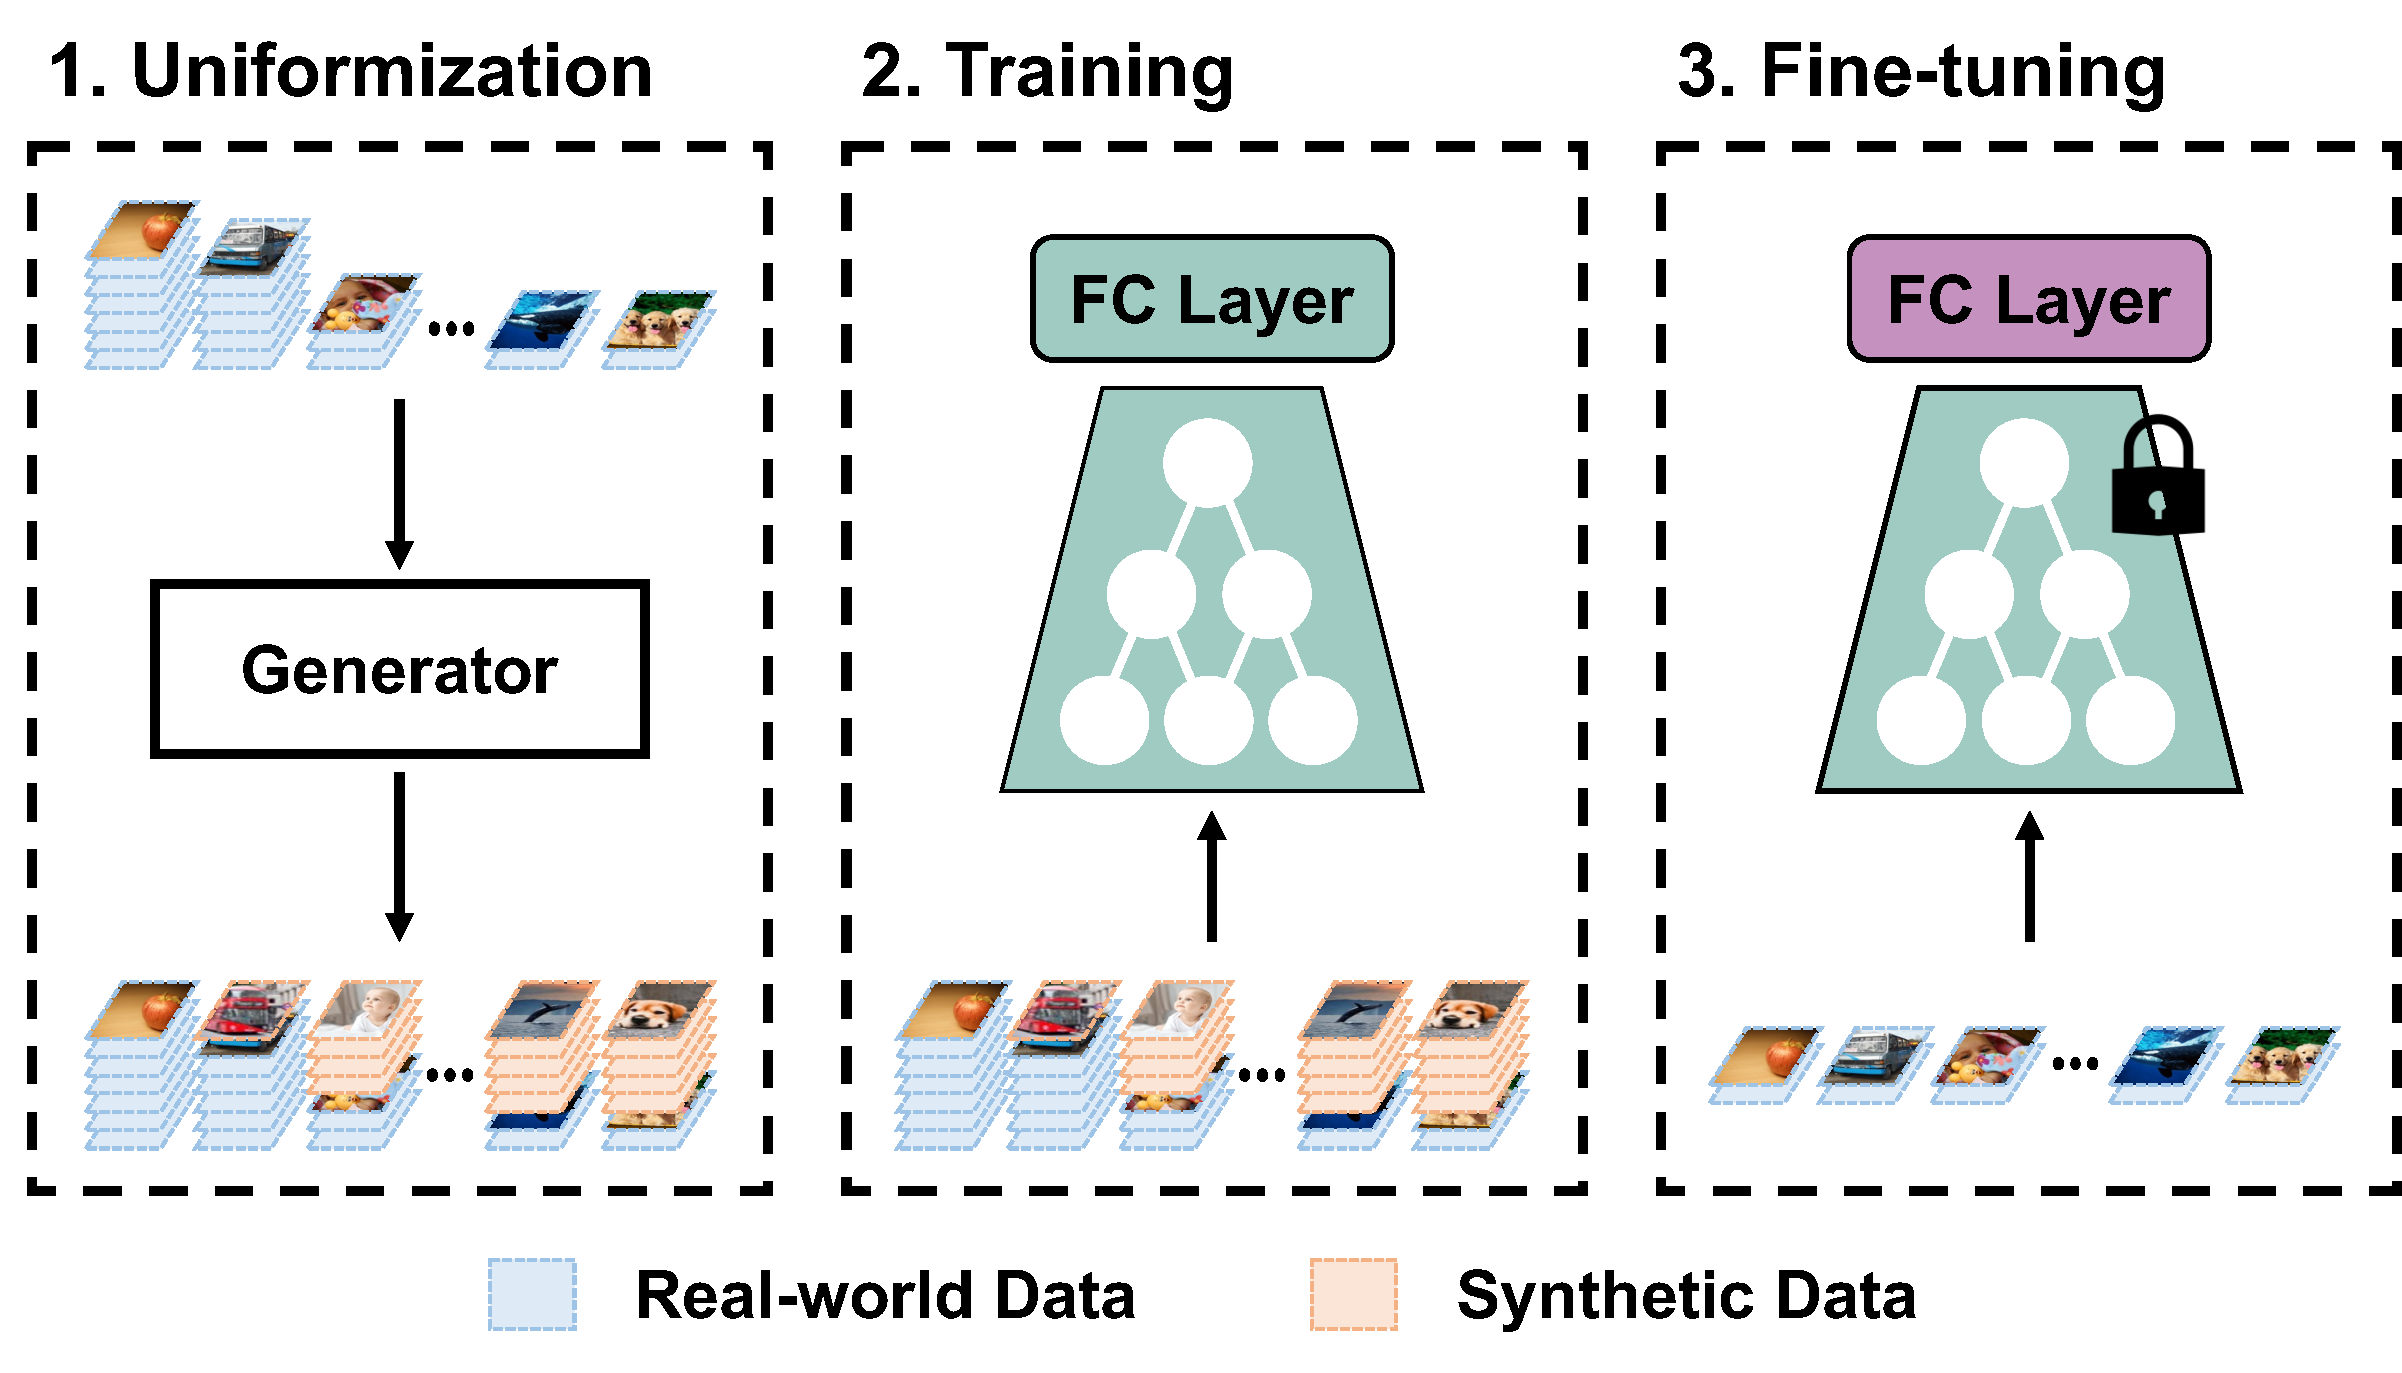
\includegraphics[width=1.0\linewidth]{figures/final.pdf}
    \caption{\textbf{Overview of SYNAuG process.}
    % \textcolor{realblue}{\textbf{legenBlue}} is the real-world data, and \textcolor{synorange}{\textbf{orange}} is the synthetic data.
    Given the imbalanced real-world data with the class labels, we first uniformize the imbalanced real data distribution by generating the synthetic samples that are conditioned on the class label.
    Second, we train a model with the uniformized training data.
    Finally, we fine-tune the last layer with the uniformly subsampled real-world data.}
    \label{fig:overview}
\end{figure}

In this work, we first uniformize the number of samples in each class using the recent text-to-image generative models before applying off-the-shelf task-specific algorithms.
% This takes a different direction, unlike the prior methods.
The prior studies 
% have reported improved performance over the state-of-the-art in their respective tasks.
% However, they use
work the limited, fixed, and bounded original dataset without adding more additional data and mainly focus on algorithmic approaches, such as reweighting~\cite{cao2019learning,ren2020balanced,samuel2021distributional,huang2019deep, ben2009robust, sagawa2019distributionally, jung2023reweighting}, resampling~\cite{shen2016relay,park2022majority,kim2020m2m,liu2019large, kamiran2012data, idrissi2022simple, roh2020fairbatch}, or augmentation~\cite{chuang2021fair, kim2020m2m, park2022majority}.
In contrast to the prior arts, we go beyond the fixed original dataset by exploiting
% , we exploit 
the generative diffusion models to synthesize data, which have recently shown potential as synthetic training data generation~\cite{poole2023dreamfusion, raj2023dreambooth3d, chen2023fantasia3d,trabucco2023effective, he2022synthetic, azizi2023synthetic}.
This allows us to tackle the fundamental bottleneck of data imbalance, \ie, data, rather than indirect ways of tackling learning algorithms or architectures.
It is a more natural way than restricting training data to the fixed dataset as in the prior arts.
% , which would be unnecessary in the generative model era.
% In the generative model era, we argue that restricting training data to the fixed dataset is impractical.
% Furthermore, data imbalance problems should be tackled from the data level before deploying algorithmic approaches.
% so that the practitioners take the controllability of data to mitigate and stabilize the base conditions of datasets.

As shown in \Fref{fig:overview}, we propose SYNAuG, exploiting the generative diffusion model to augment and make the original data distribution to be uniform distribution, \ie, uniformization.
% uniformize the original training data.
% , motivated by recent class imbalance approaches~\cite{kim2020m2m,he2022synthetic,kirichenko2023last}.
After training on the uniformized data composed of the original and synthetic data, we found that it is effective to use simple fine-tuning of the last layer with uniformly sub-sampled original data.
% after pretraining on the mixed dataset.
This outperforms the other strong baselines, including the baseline using the additional external web data as well as the competing methods on the long-tailed recognition benchmark, CIFAR100-LT, and the fairness benchmark, UTKFace.
In addition, we demonstrate the effectiveness of our method for improving the robustness of the classifier to spurious correlation.
We summarize our contributions as follows:
\begin{itemize}
    \item Proposing SYNAuG that uniformizes the given data distribution with synthetic data, beyond the given datasets;\vspace{-1mm}
    % not restricted to the given datasets;
    \item Demonstrating the effectiveness of SYNAuG on three distinctive data imbalance tasks: long-tailed recognition, model fairness, and robustness to spurious correlation;
    \vspace{-1mm}
    \item Reporting the observation of the importance of a few original samples when we use synthetic data together.
\end{itemize}




%-------------------------------------------------
\section{Related Work}\label{sec:rw}


% \paragraph{Data Imbalance Problems.}
% In the real world, dogs and cats outnumber rare animals, and this characteristic of nature is reflected in the curation of data.
% These data imbalance problems can cause poor generalization and many issues in finance, healthcare, and autonomous driving.
% In this paper, we tackle long-tailed recognition, fairness, and model robustness to spurious correlation, which are related closly from the data imbalacne perspective.

% Imbalance in data
Data imbalance can lead to
% cause poor
suboptimal generalization and many challenges
% issues
in practical application scenarios, \eg, finance, healthcare, and autonomous driving.
The data imbalance problem is a common source of different imbalance sub-problems: long-tailed recognition, model fairness, and model robustness to spurious correlation.
% This work is related to the data imbalance problem, and 
We brief the related work on the associated sub-problems and on using synthetic data for machine learning tasks.
% review its associated sub-problems and using synthetic data.
% : class imbalance (long-tail), fairness, and spurious correlation.
% In this paper, we tackle which are related closly from the data imbalacne perspective.



% \begin{wrapfigure}{r}{0.45\linewidth}
%     \centering
%     \vspace{-6mm}
%     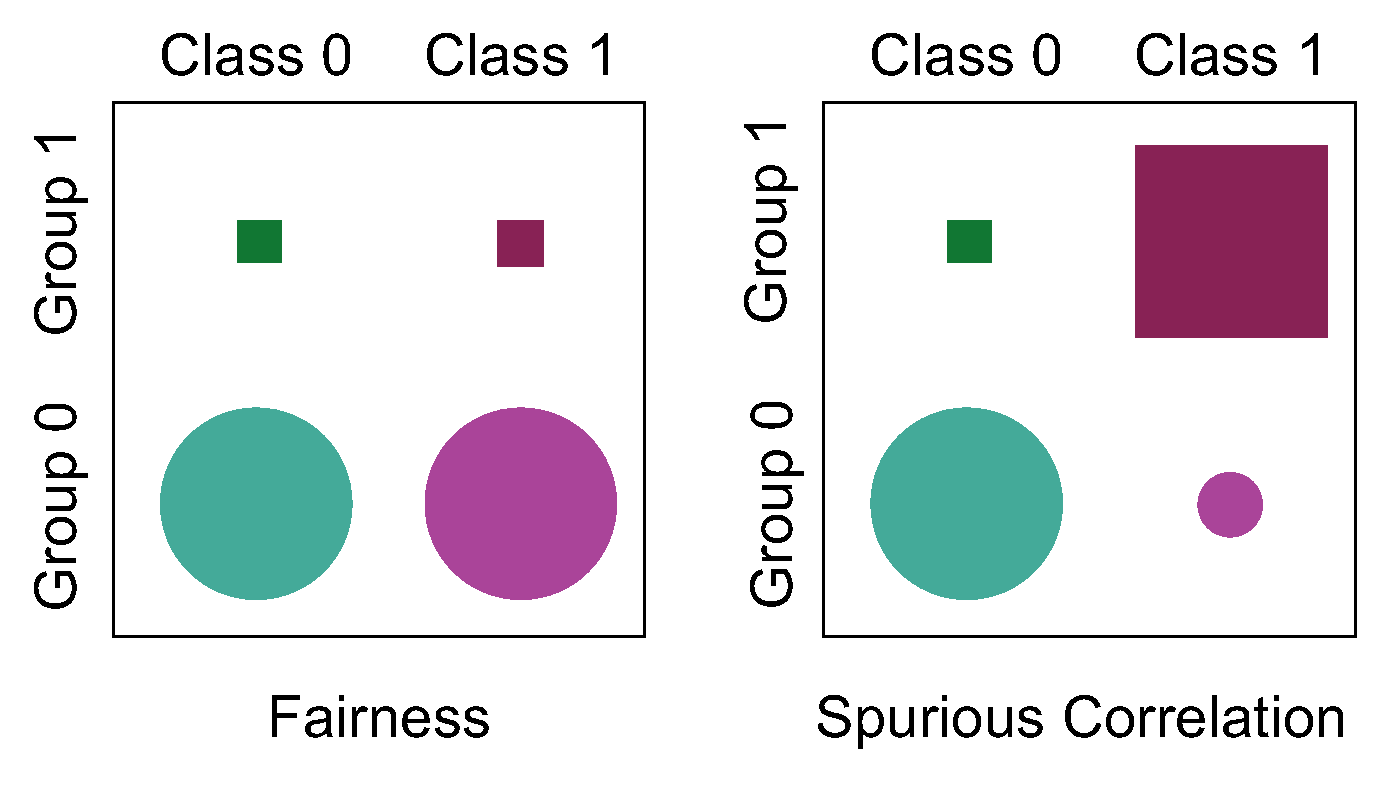
\includegraphics[width=1.0\linewidth]{figures/group_imbalance_teaser.pdf}
%     \caption{\textbf{Overview of fairness and spurious correlation from the data perspective.}
%     The size of a shape represents the amount of data. The same shape stands for the same group, and the same color for the same class.\vspace{-3mm}}
%     % 
%     \label{fig:group_imbalance_teatures}
% \end{wrapfigure}

% It is well-known that long-tailed recognition~\cite{cui2019class,zhang2023deep}, where their training data follow Pareto distribution, is one of the class imbalance problems.
% Long-tailed distribution, \ie, Pareto distribution, is natural in the real world, which has a class imbalance.
% Dogs and cats outnumber rare animals, and this characteristic of nature is reflected in the curation of data.


% (see \Fref{fig:group_imbalance_teatures}).

% Model robustness is related to spurious correlations that some classes appear with certain patterns, \ie, spurious or shortcut features~\cite{geirhos2020shortcut, scimeca2022iclr, kirichenko2023last}.

% for deep neural networks 

% Since the long-tail distribution, model robustness, and model fairness are related closely from the data imbalance perspective, we handle these three data imbalance problems.



\paragraph{Long-tailed recognition.}
Long-tailed distribution is inherent to the real world~\cite{cui2019class,zhang2023deep}.
There are two main streams in the realm of re-balancing classes, including re-sampling~\cite{shen2016relay,park2022majority,kim2020m2m,liu2019large} and re-weighting~\cite{he2009learning,samuel2021distributional, cao2019learning, ren2020balanced, lin2017focal, ryou2019anchor, cui2019class}.
The re-weighting methods share a similar mechanism to weighting minority classes inverse-proportionally to the number of instances. 
% less frequent class by the inverse of frequency~\cite{he2009learning, cui2019class}.
The re-sampling methods weight the samples in minority classes by more frequently sampling with replacement so that the training model can see the uniform number of samples across classes.

There are other approaches 
% to tackle the problem
by designing loss functions.
Ryou~\etal\cite{ryou2019anchor} and Lin~\etal\cite{lin2017focal} 
% design loss functions that 
induce adaptive re-weighting effects during training.
The others take into account margin~\cite{cao2019learning} or balance of softmax~\cite{ren2020balanced} in the loss design.
% Also, there are other approaches to take into account other factors in the loss design: margin~\cite{cao2019learning} or balance of softmax~\cite{ren2020balanced}.
Wang~\etal\cite{wang2021longtailed} take a completely different approach; model selection given diversely pre-trained classifiers.
In addition, Ye-Bin~\etal\cite{yebin2023textmania} propose
% proposes
TextManiA, visual feature augmentation for sparse samples, which shows improved performance in long-tailed distribution.


\paragraph{Model fairness.} 
In fairness~\cite{narayanan2018translation, hardt2016equality, 10.1145/2783258.2783311}, researchers have tackled the issue of model bias, where accuracy varies based on 
% the unfairness that the model accuracy is different depending on
sensitive attributes such as race, age, and ethnicity.
Model fairness is also related to data imbalance because the number of samples of some sensitive groups is lower than that of the major groups.
Fairness has predominantly been tackled using loss weighting and batch sampling.
A loss weighting algorithm~\cite{jung2023reweighting} proposes fairness optimization, where they minimize the worst-case loss of the group by adaptively weighting losses.
% during training.
Batch sampling approaches~\cite{kamiran2012data, roh2020fairbatch} take an adaptive sampling strategy by considering sensitive information rather than uniform sampling.
Zeng~\etal\cite{zeng2022fair} take a post-calibration approach after training
% with the above existing method
to calibrate the classifiers.


% arjovsky2019invariant,bahng2020learning,sagawa2019distributionally,teney2020unshuffling,tartaglione2021end, lee2021learning,LfF,liu2021just, kim2022learning,yao2022improving,hwang2022selecmix,kirichenko2023last,cao2019learning,ren2020balanced,samuel2021distributional, shen2016relay,park2022majority,kim2020m2m,liu2019large
\paragraph{Spurious correlation.}
% While the spurious correlation problem shares similarities with fairness, it 
The spurious correlation problem is related to the robustness of models against misleading correlations.
DNNs are susceptible to falling into shortcuts that capture the most frequently observed patterns in a class regardless of true causality;
it is called spurious correlation or shortcut problems~\cite{geirhos2020shortcut, scimeca2022iclr, kirichenko2023last}.
It is never desirable to rely on spurious features that degrade the generalizability of DNNs~\cite{sagawa2019distributionally, liu2015deep}.
The spurious correlation problem is also dealt with similar approaches to the above two tasks: weighting~\cite{sagawa2019distributionally,LfF,kim2022learning}, sampling~\cite{idrissi2022simple, sagawa2020investigation}, augmentation~\cite{lee2021learning,yao2022improving,hwang2022selecmix}, and post-calibration~\cite{liu2021just, kirichenko2023last, lee2022surgical}.


\paragraph{Summary of data imbalance problems.}
While researchers have developed algorithms for each task separately, three different tasks sourced from data imbalance have mainly been tackled in the shared perspective, \ie, 
% re-balancing; 
up-weight loss values or sampling probabilities of minor groups using group or sensitive information.
However, they have focused only on algorithmic parts by limiting their methods to exploit the given imbalance dataset, where the inherent imbalance still remains.

In this work, we shed light on the overlooked convention to go beyond the given bounded dataset.
We exploit the synthetic data from the generative foundation models~\cite{rombach2022high, saharia2022photorealistic, nichol2021glide} to take flexibility and controllability so that we can populate the long-tailed training data distribution to become a uniform distribution, which mitigates the imbalance problem itself.
We observe that this simple correction of class distribution with synthetic data can significantly improve the worst-case accuracy and fairness of DNNs.
To our best knowledge, our work is the first work that demonstrates improved or competitive performance with generated synthetic data for both class imbalance and fairness tasks.

\paragraph{Using synthetic data in machine learning tasks.}
To overcome the lack of data or sensitive issues of data, \eg, licensing and privacy concerns, recent approaches have started to leverage synthetic data for their tasks of interest:
classification~\cite{antoniou2017data, tran2017bayesian}, segmentation~\cite{sandfort2019data, zhang2021datasetgan}, re-identification~\cite{zheng2017unlabeled}, motion estimation~\cite{dosovitskiy2015flownet, mayer2016large, sun2021autoflow, han2022realflow, oh2018learning}, computational photography~\cite{pan2021dual}, and representation learning~\cite{jahanian2021generative}.
Recently, deep generative models~\cite{rombach2022high, saharia2022photorealistic, nichol2021glide} have shown promising results in generating realistic and high-quality samples, stemming from the goal of modeling the real data distribution.
In particular, the image generation conditioned on text provides great controllability and flexibility, which has the potential to be used for a variety of tasks, such as 3D reconstruction~\cite{poole2023dreamfusion, raj2023dreambooth3d, chen2023fantasia3d} and image recognition~\cite{trabucco2023effective, he2022synthetic, azizi2023synthetic}.
In this work, we explore the use of a pre-trained foundation diffusion model to mitigate data imbalance problems.




%-------------------------------------------------
\section{Method}\label{sec:synaug}

We first present our motivation for using synthetic data to address data imbalance problems based on experimental findings (\Sref{sec:2.1}).
Building on these empirical insights, we propose to exploit the synthetic data (SYNAuG) as a means to uniformize the given training data distribution 
% of the given training data
(\Sref{sec:2.2}).
% Note that we do not advocate that SYNAuG is a solution for the data imbalance problem, but it provides a novel perspective from a data point of view.

\begin{figure}
    \centering
        \begin{subfigure}[b]{0.9\linewidth}
        \centering
        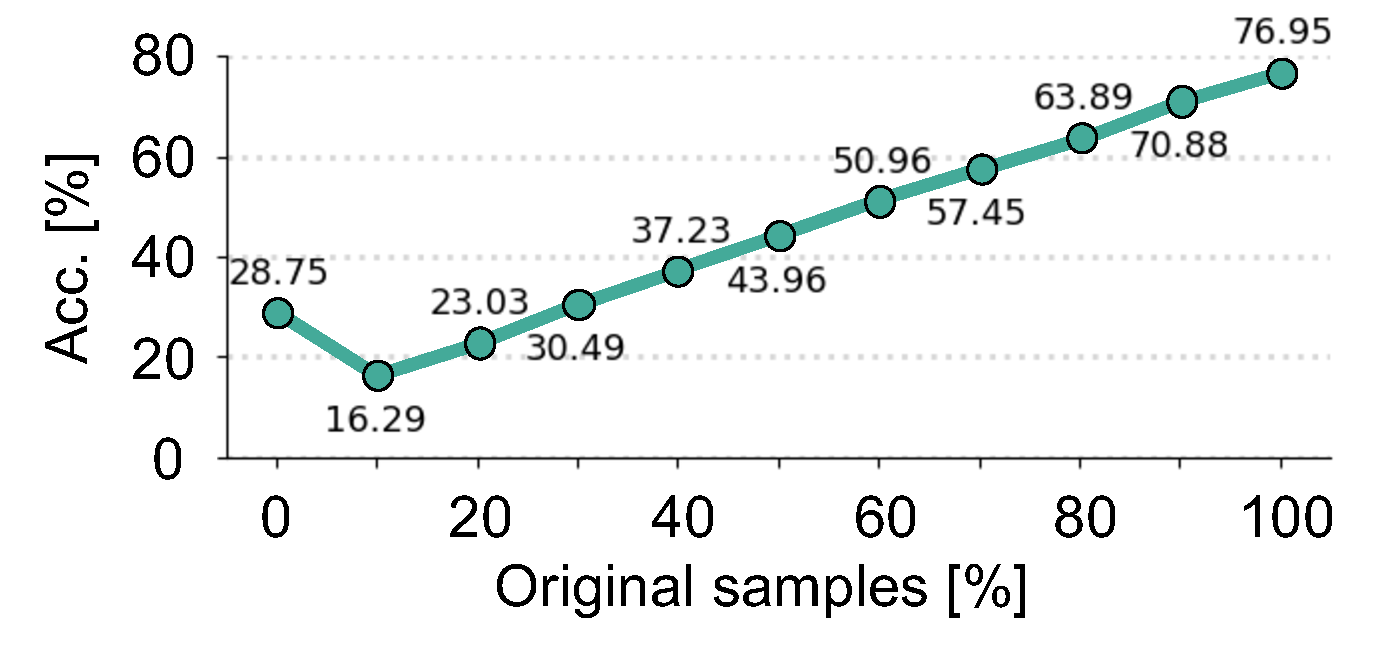
\includegraphics[width=1.0\linewidth]{figures/example1.pdf}
        \caption{Class-wise replacement}
        \label{fig:classwise}
    \end{subfigure}
    \centering
        \begin{subfigure}[b]{0.9\linewidth}
        \centering
        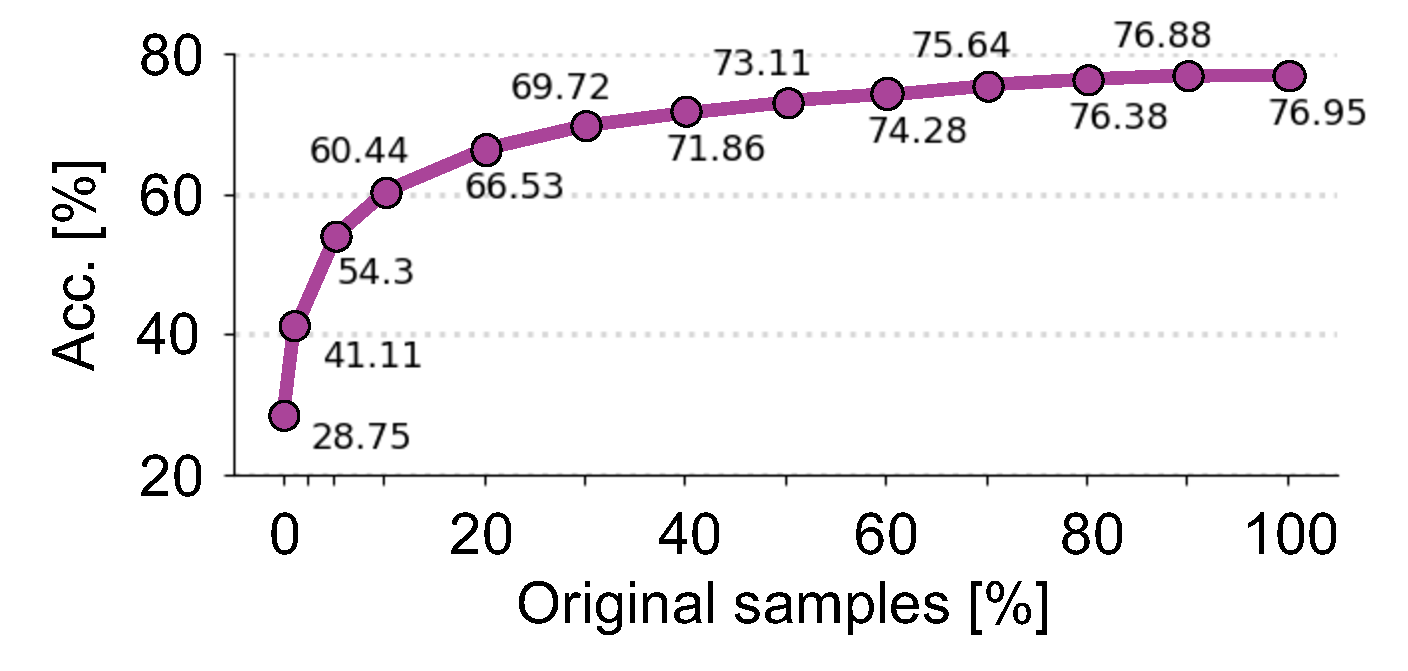
\includegraphics[width=1.0\linewidth]{figures/example2.pdf}
        \caption{Instance-wise replacement}
        \label{fig:instwise}
    \end{subfigure}    
    \caption{\textbf{Replacement test.} 
    To investigate the effect on model performance when using original and synthetic data together, we replace the original data with synthetic ones in two ways: (a) class-wise and (b) the same ratio of instances across all classes.
    We use CIFAR100, which has 500 samples per class and 100 classes.
    }
    \label{fig:abl_ratio}
\end{figure}

\subsection{Motivations}\label{sec:2.1}
During training, we consider how to curate the data, train the model, and evaluate it.
As aforementioned, prior methods addressing data imbalance problems have explored in various ways, including data re-sampling, loss function design, and model architecture.
Instead, 
% As the first step, data curation significantly affects the training and the subsequent evaluation.
we emphasize the importance of data curation and the controllability of data, as data curation significantly affects the training and the subsequent evaluation despite its position as the first step.
% In this work, we propose to utilize the power of the recent text-to-image generative model, which provides controllability in generating synthetic samples.

Before incorporating synthetic data into our proposed method, we delve into the influence of training with synthetic and original data together.
We establish two settings by controlling the ratio of original and synthetic data.
We use the generated images from the Stable Diffusion~\cite{rombach2022high} for synthetic data.
In the \textbf{first setting}, we take an extreme approach by replacing whole original data belonging to specific classes with synthetic data.
It means that certain classes have no real samples but only synthetic samples.
% , and this setting is an extreme case of data imbalance.
In the \textbf{second setting}, we uniformly replace the original data with synthetic data, which means all classes have the same ratio of original and synthetic data.
This approach ensures that every class at least has a few original data.
The significance of original samples becomes apparent through observing the performance change.

% Figure~\ref{fig:abl_ratio} shows t
The results of the two settings are in \Fref{fig:abl_ratio}.
The first setting shows the linear performance degradation as the number of classes with no original data increases (See \Fref{fig:classwise}).
However, the second setting shows the log-like performance degradation as more original data are replaced with synthetic data uniformly (See \Fref{fig:instwise}).
We achieve 41.11\% when using 1\% of real data in the second setting, which is similar to the result of 43.96\% when using 50\% of real data in the first setting.
% The performance of 1\% of real data in the second setting is 41.11\%, which is similar to the performance of 50\% of real data in the first setting, 43.96\%.
%It indicates that few original samples might be needed. and the domain gap might exist despite high-quality synthetic data.
% 어감이 few original samples 이 앵커 역할을 한다는거면 조금 더 강조를 해야할수도..
The results suggest that at least a few original samples are necessary as an anchor, as
% while
the domain gap may still exist even with high-quality synthetic data.
% In addition, the performance difference between 100\% and $n$\% accuracies in \Fref{fig:instwise} would represent the existence of the domain gap between real and synthetic data.

\begin{figure}
    \centering
        \begin{subtable}[c]{0.3\linewidth}
        \centering
        \resizebox{1.0\linewidth}{!}{
            \begin{tabular}{cc}
                \toprule
                & \textbf{Accuracy} \\ 
                \midrule
                Real  & 77.76 \\
                Syn.  & 70.56 \\
                \cmidrule{1-2}
                Total & 74.16 \\
                \bottomrule 
            \end{tabular}
        }
        \caption{Binary domain classification}    
        \label{fig:domain_cls}
    \end{subtable}
    \hspace{8mm}
    \centering
        \begin{subfigure}[c]{0.5\linewidth}
        \centering
        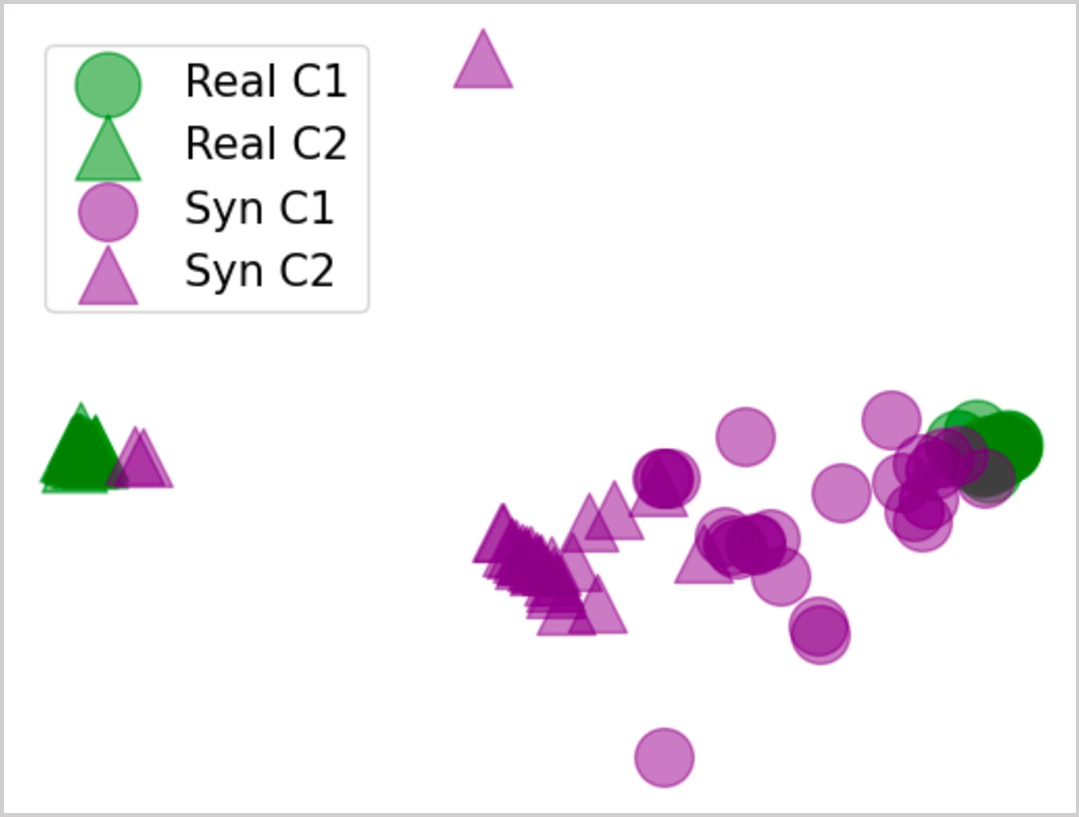
\includegraphics[width=1.0\linewidth]{figures/domain_gap.pdf}
        \caption{Feature visualization}
        \label{fig:domain_feat}
    \end{subfigure}    
    \caption{\textbf{Domain gap between real and synthetic data.} 
    We test the domain gap empirically with (a) binary domain classification and (b) feature visualization.
    For binary classification, we use 2.5k samples for each real and synthetic domain and train only one fully-connected layer with the extracted features.
    For visualization, the features are extracted from the pre-trained model on CIFAR100.
    % , a total of 5k samples.
    % We first train the model with real samples (CIFAR100) and re-train the last layer from scratch to classify the given samples as real or synthetic. 
    % For re-training, we use 2.5k samples for each real and synthetic domain, a total of 5k samples.
    % The features are extracted before the last layer.
    C1 and C2 denote different classes.
    }
    \label{fig:domain}
\end{figure}

To check the presence of a domain gap, we conduct domain classification and visualization of the features from both real and synthetic data (See \Fref{fig:domain}).
As shown in \Fref{fig:domain_cls}, the classification performance is 74.16\%.
This indicates the existence of a domain gap, considering that 50\% means no domain gap.
As shown in \Fref{fig:domain_feat}, the features of Syn C2 are more closer to Syn C1 rather than Real C2.
% the features of synthetic data in class 1 (Syn C1) are closer than features of real data. 
% \wonseok{As shown in \Fref{fig:domain_feat}, the features of synthetic data are more tightly clustered than the features of real data. }
This observation provides empirical evidence of a domain gap existing between real and synthetic data.

% If there is no domain gap between real and synthetic data, the domain classifier would be incapable of distinguishing between samples, yielding an accuracy of 50\%.
% However, as depicted in Figure \ref{fig:domain_cls}, the obtained accuracy of 74.16\% indicates a discernible domain gap.
% Visualization result depicted in \Fref{fig:domain_feat} reveals that some of the synthetic samples are distant from their corresponding real samples within the same class.
% This observation also provides empirical evidence of a domain gap existing between real and synthetic data.

In summary, (1) at least, a few real samples are important when we supplement the real samples with the synthetic samples,
(2) synthetic samples are still insufficient to fully replace the original samples, although the deep generative models show impressive performance,
thus, (3) there might be additional room for improvement due to the domain gap between the original and the synthetic data.
It is desirable that the remaining original samples serve as an anchor role, and synthetic data support and populate the insufficient samples.

% While the first case shows the linear performance degradation as shown in \Fref{fig:classwise}, the second case shows the performance degradation alleviate rather than the first case as shown in \Fref{fig:instwise}.
% Interestingly, the performance of 1\% of original data in the second case is similar to the performance of 50\% of original data in the first case.
% In addition, the performance difference between 100\% and $n$\% accuracies in \Fref{fig:instwise} would represent the existence of the domain gap between original and synthetic data in a same class.
% These results imply that (1) synthetic data is still insufficient to replace original data fully, (2) we need a few original samples when supplementing the original data with the synthetic data, and (3) there might be additional room for improvement due to the domain gap between the original and the synthetic data.
% It is desirable that the remaining original samples serve as an anchor role, and synthetic data support and populate the insufficient samples.





\subsection{SYNAuG}\label{sec:2.2}
Given the preliminary experiments, we propose SYNAuG, which leverages synthetic data to mitigate the imbalance and domain gap from the data perspective.
Our approach is applied to 
% across
three distinct tasks: long-tailed recognition, model fairness, and robustness to spurious correlation.
While these tasks differ in their ultimate objectives and evaluation metrics, the common underlying factor is the presence of data imbalance.
SYNAuG is an integrated approach designed to mitigate data imbalance across diverse tasks.

As illustrated in \Fref{fig:overview}, we first uniformize the imbalance data by generating synthetic data, train the model on the uniformized data, and finally fine-tune the last layer with a few original data uniformly subsampled from each class.
% original data.
We exploit recent powerful generative models, \eg, Stable Diffusion~\cite{rombach2022high}, to generate the synthetic data of corresponding classes or attributes with the controllable prompt.
Since they are trained on a large number of web data, it would be considered to cover and model the wide distribution of the real world.
Exploiting these favorable properties, we generate supporting data to alleviate the imbalance of the data distribution.
We generate the samples with diverse prompts like ``a photo of \{\texttt{modifier}\} \{\texttt{class}\}''.
% 개인적으로 이게 조금 더 깔끔한 느낌
%We can find the modifier by humans but use ChatGPT~\cite{ouyang2022training} to make our pipeline automatic.
We find list of proper modifiers by ChatGPT~\cite{ouyang2022training} to make our pipeline automatic.
% With the data uniformized according to the target imbalance axis, w
We train the model on uniformized data with Cross Entropy (CE) loss.

While SYNAuG is simple and effective, there is still room to improve its performance because of the domain gap identified 
% , as mentioned
in \Sref{sec:2.1}.
% because the domain gap exists between original and synthetic data, as we mentioned in \Sref{sec:2.1}.
To bring further improvement by mitigating the gap, we propose to utilize two simple methods.
% , as shown in \Fref{fig:overview}.
First, we propose to leverage
% use
Mixup~\cite{zhang2017mixup} during training to augment the samples to be interpolated samples between real and synthetic samples, \ie, domain Mixup.
Second, we propose to fine-tune the classifier on the subsampled uniform original data from the original training data after the first training stage.
% Our experiment show that t
The fine-tuned classifier would lead to more accurate recognition of the target data by alleviating the domain gap.

% 361-364에 거의 똑같은 내용이 있어서, 한번 더 써서 강조하는 느낌을 준다면 조금 더 요약하는 느낌을 주는건? To summarize, our proposed method ~
% Note that our method exploits synthetic data to address the imbalance problem from the data perspective, leveraging the data controllability of synthetic data. 
In summary, the process of SYNAuG is as follows:
%Note that based on data controllability, our method exploits the synthetic data to tackle the imbalance problem from the data point of view. The process of SYNAuG is as follows: 
(1) uniformize the original data distribution with synthetic data from the generative model, (2) train the model with uniformized data using Mixup, and (3) fine-tune the last layer with the uniformly subsampled real data.



%-------------------------------------------------
\section{Experiments}

In this section, 
% we demonstrate the effectiveness of SYNAuG for data imbalance problems.
we evaluate our method for three sub-tasks: long-tailed recognition task (\Sref{sec:lt}), model fairness (\Sref{sec:fairness}), and model robustness to spurious correlation (\Sref{sec:robustness}).
% Additional results and details can be found in the supplementary material.
Through these results, we demonstrate the effectiveness of SYNAuG for data imbalance problems.

\subsection{Long-tailed Recognition}\label{sec:lt}

\begin{table*}[t]
\centering
\resizebox{0.65\linewidth}{!}{
    \begin{tabular}{@{}lcccccc}
        \toprule
        \multirow{2}[2]{*}{\textbf{{Method}}} & \multicolumn{4}{c}{\textbf{IF=100}} & \multirow{2}[2]{*}{\textbf{{50}}} & \multirow{2}[2]{*}{\textbf{{10}}} \\
        \cmidrule{2-5}
        & \textbf{Many} & \textbf{Medium} & \textbf{Few} & \textbf{All} & & \\
        \midrule
        CE~\cite{cui2019class}                         & 68.31 & 36.88 & 4.87 & 37.96 & 43.54 & 59.50 \\
        \cmidrule{1-7}
        SSD~\cite{li2021self}                          & - & - & - & 46.0 & 50.5 & 62.3 \\
        PaCo~\cite{cui2021parametric}                  & - & - & - & 52.0 & 56.0 & 64.2 \\
        RISDA~\cite{chen2022imagine}                   & - & - & - & 50.16 & 53.84 & 62.38 \\
        CE + CMO~\cite{park2022majority}               & 70.4 & 42.5 & 14.4 & 43.9 & 48.3 & 59.5 \\
        LDAM + CMO~\cite{park2022majority}             & 61.5 & 48.6 & 28.8 & 47.2 & 51.7 & 58.4 \\
        RIDE (3 experts) + CMO~\cite{park2022majority} & - & - & - & 50.0 & 53.0 & 60.2 \\
        Weight Balancing~\cite{alshammari2022long}     & 72.60 & 51.86 & 32.63 & 53.35 & 57.71 & 68.67 \\
        \cmidrule{1-7}
        % Web crawled images                        & 72.71 & 51.21 & 36.13 & 54.06 & 56.40 & 63.86 \\
        % \cmidrule{1-7}
        % Intra-class Image Translation             & 71.86 & 45.88 & 22.97 & 47.87 & 53.33 & 64.95 \\
        % Inter-class Image Translation             & 73.49 & 45.77 & 19.00 & 47.17 & 51.33 & 64.11 \\
        % Class Distribution Fitting                & \textbf{74.83} & 50.79 & 26.03 & 51.53 & 55.60 & 65.60 \\
        % \cmidrule{1-7}
        SYNAuG                                    & \textbf{74.06} & \textbf{56.63} & \textbf{42.83} & \textbf{58.59} & \textbf{61.36} & \textbf{69.01} \\
        % SYNAuG                                         & 74.66 & 52.21 & 27.52 & 52.41 & 56.99 & 66.34 \\
        % SYNAuGAttr                                     & 75.23 & 52.15 & 30.58 & 53.54 & 57.09 & 66.66 \\
        % SYNAuG + Mixup                                 & 75.37 & 54.24 & 32.16 & 54.79 & 57.55 & 66.66 \\
        % SYNAuGAttr + Mixup                             & 74.97 & 53.77 & 35.26 & 55.45 & 58.69 & 66.84 \\
        % SYNAuGAttr + classifier re-training            & 74.83 & 52.57 & 33.13 & 54.53 & 57.93 & 66.80 \\
        % SYNAuGAttr + classifier fine-tuning            & 74.43 & 53.26 & 32.97 & 54.58 & 58.26 & 67.24 \\
        % SYNAuGAttr + Mixup + classifier re-training    & 73.97 & 56.26 & 39.10 & 57.31 & 60.34 & 67.90 \\
        % SYNAuGAttr + Mixup + classifier fine-tuning    & 74.06 & 56.63 & 42.83 & 58.59 & 61.36 & 69.01 \\
        \bottomrule 
    \end{tabular}
    }
    \caption{\textbf{Long-tailed recognition performance on CIFAR100-LT.}
    We compare our SYNAuG with recent works in long-tailed recognition.
    We report the Top-1 accuracy (\%) with different imbalance factors, \ie, IF=\{100, 50, 10\}.
    % \textbf{Bold} stands for the highest accuracy in each IF or class.
    }
    \label{tab:cifar100_lt}
\end{table*}

\begin{table}[t]
\centering
\resizebox{1.0\linewidth}{!}{
    \begin{tabular}{@{}lcccc}
        \toprule
        \multirow{2}[2]{*}{\textbf{{Method}}} & \multirow{2}[2]{*}{\textbf{\makecell{Additional\\Data Type}}}& \multicolumn{3}{c}{\textbf{IF}} \\
        \cmidrule{3-5}
        & & \textbf{100} & \textbf{50} & \textbf{10}\\
        \midrule
        CE~\cite{cui2019class} & N/A & 37.96 & 43.54 & 59.50 \\                        
        % & 68.31 & 36.88 & 4.87 & 37.96 & 43.54 & 59.50 \\
        \cmidrule{1-5}
        Web crawled images    & Real & 54.06 & 56.40 & 63.86 \\
        % & 72.71 & 51.21 & 36.13 & 54.06 & 56.40 & 63.86 \\
        \cmidrule{1-5}
        Intra-class Image Translation & Syn. & 47.87 & 53.33 & 64.95 \\
        % & 71.86 & 45.88 & 22.97 & 47.87 & 53.33 & 64.95 \\
        Inter-class Image Translation & Syn. & 47.17 & 51.33 & 64.11 \\
        % & 73.49 & 45.77 & 19.00 & 47.17 & 51.33 & 64.11 \\
        Class Distribution Fitting     & Syn. & 51.53 & 55.60 & 65.60 \\
        % & \textbf{74.83} & 50.79 & 26.03 & 51.53 & 55.60 & 65.60 \\
        \cmidrule{1-5}
        SYNAuG                          & Syn. & \textbf{58.59} & \textbf{61.36} & \textbf{69.01} \\
        % & 74.06 & \textbf{56.63} & \textbf{42.83} & \textbf{58.59} & \textbf{61.36} & \textbf{69.01} \\
        \bottomrule 
    \end{tabular}
    }
    \caption{\textbf{Comparison with the baselines.}
    We use CIFAR100-LT.
    The second column denotes the data type used in uniformization.
    % with different imbalance factors, \ie, IF=\{100, 50, 10\}.
    % \textbf{Bold} stands for the highest accuracy in each IF or class.
    }
    \label{tab:cifar100_lt_baseline}
\end{table}


\begin{table}[t]
\centering
\resizebox{1.0\linewidth}{!}{
    \begin{tabular}{cccccccc}
        \toprule
        \multirow{2}[2]{*}{} & \multirow{2}[2]{*}{\textbf{Modifier}} & \multirow{2}[2]{*}{\textbf{Mixup}} & \multirow{2}[2]{*}{\textbf{Re-train}} & \multirow{2}[2]{*}{\textbf{Finetune}} & \multicolumn{3}{c}{\textbf{IF}} \\ \cmidrule{6-8}
        & & & & & \textbf{100} & \textbf{{50}} & \textbf{{10}} \\
        \midrule
        (a) & & & & & 52.41 & 56.99 & 66.34 \\
        (b) & \checkmark & & & & 53.54 & 57.09 & 66.66 \\
        % (c) & & \checkmark &  & 54.79 & 57.55 & 66.66 \\
        (c) & \checkmark & \checkmark & & & 55.45 & 58.69 & 66.84 \\
        (d) & \checkmark & \checkmark & \checkmark & & 57.31 & 60.34 & 67.90 \\
        (e) & \checkmark & \checkmark & & \checkmark & \textbf{58.59} & \textbf{61.36} & \textbf{69.01} \\
        \bottomrule 
    \end{tabular}
    }
    \caption{\textbf{Ablation study of SYNAuG.} 
    We use CIFAR100-LT.
    Each component, Modifier, Mixup, Re-train, and Finetune, means we use the class-related modifiers in the prompt, use Mixup augmentation during training, and re-train or finetune the last layer after training, respectively.
    (e) stands for our SYNAuG.
    }
    \label{tab:ablation}
\end{table}



\paragraph{Experimental setting.}
We employ two long-tail datasets: CIFAR100-LT~\cite{cao2019learning} and ImageNet100-LT~\cite{jiang2021self}.
CIFAR100-LT and ImageNet100-LT have train sets that are artificially curated to make class imbalance from the original datasets, CIFAR100~\cite{krizhevsky2009learning} and ImageNet100~\cite{tian2020contrastive}.
The test sets for them are the same as the original one.
The classes in the long-tailed datasets are divided into three groups: Many-shot (more than 100 samples), Medium-shot (20-100 samples), and Few-shot (less than 20 samples).
For CIFAR100-LT, the imbalance factor (IF) can be controlled by computing the ratio of samples in the head to tail class, $N_1/N_K$, where $N_k=\left| \mathcal{D}_k\right|$, and $\mathcal{D}_k$ is the set of samples belonging to the class $k\in\{1,\cdots,K\}$.
As the IF value increases, the skewness of the training data becomes more severe, which makes it more challenging.
%When the IF value is large, the skewness of the training data is more severe, which has fewer samples and is more challenging.
We evaluate under the standard IFs of 100, 50, and 10, following~\cite{alshammari2022long}.
We use ResNet32 for CIFAR100-LT and ResNet50 for ImageNet100-LT.
Further details can be found in the supplementary material.


\paragraph{Competing methods and baselines.}
We compare with recent prior arts: SSD~\cite{li2021self} and PaCo~\cite{cui2021parametric} for self-supervised learning, RISDA~\cite{chen2022imagine} and CMO~\cite{park2022majority} for data augmentation, and Weight Balancing~\cite{alshammari2022long} for the rebalance classifier.
They are state-of-the-art in each perspective and propose methods only using 
% limited to 
the original long-tailed data without external data sources.
% As a strong baseline in terms of data supplement perspective, we collect the data from the internet to populate the insufficient samples, named as WebAug.

We present other 
% baselines by using 
variants of generation methods as baselines:
1) Motivated by the recent work~\cite{he2022synthetic} using the few-shot original samples as guidance during the generation process, we first introduce
% For 
\emph{Intra-class Image Translation}, where we use the original samples from the original training data as a class-wise guidance image for generation,
% It is motivated by the recent work~\cite{he2022synthetic} using the few-shot original samples as guidance during the generation process.
2) Inspired by the M2m~\cite{kim2020m2m} translating an image of the major class to the minor class for leveraging the diversity of the majority information, we introduce
% For 
\emph{Inter-class Image Translation}, where we utilize random samples in the dataset as guidance regardless of the class,
% It is inspired by the M2m~\cite{kim2020m2m} translating an image of the major class to the minor class for leveraging the diversity of the majority information.
3) As an advanced version motivated by DreamBooth~\cite{ruiz2022dreambooth}, we fine-tune the diffusion model with the samples in each class to model the class-wise distribution, named \emph{Class Distribution Fitting},
% ,\footnote{During fine-tuning, we add infrequently used text fragment, such as ``pqk'', as a class token before the target class word in the prompt.
% After fine-tuning the generative model, the added text fragment would become a token that includes the class information.
% The fine-tuned generative model generates synthetic samples for populating the training distribution.}
and 4) As a strong baseline, we collect the real data from the internet instead of generating synthetic images, \ie, \emph{Web crawled images}.
Details are in the supplementary material.


\paragraph{Comparison results.}
We compare SYNAuG with the prior arts in \Tref{tab:cifar100_lt}.
Compared to the CE method~\cite{cui2019class} trained with the Cross Entropy loss on the original data, we achieve large improvements when exploiting the generated samples regardless of the skewness of the training data.
Our method also outperforms 
% shows outperformed performance compared to 
most of the competing methods.
This is stunning results in that it
% The results 
suggests 
% demonstrates
that relieving the imbalance from the data point of view is simple but more effective than the conventional complex algorithmic methods.


In \Tref{tab:cifar100_lt_baseline}, we compare our method with our proposed baselines.
Compared to the case that uses real-world web data\footnote{We collected image from Google image search. Google image search returns images very favorable to DNNs, because Google has used CNN-based image search since March 2013~\cite{chen2015webly}. Thus, using web data is analogous to the distillation of a Google internal model, \ie, very strong baseline.}, it shows that the generated images are of sufficient quality to mitigate the class imbalance problem.
Also, we evaluate additional baselines, which apply the variant methods during the generation process.
% explained in \Sref{sec:2.3} during the generation process.
While they are better than training only with the original long-tailed data (CE method~\cite{cui2019class}), the performance is lower than SYNAuG.
The results imply that the domain gap between the original and synthetic data is hard to narrow during the generation process.
Thus, we propose to leverage 
% using
Mixup during training and fine-tuning the classifier as a more straightforward way.
Note that na\"ively applying Mixup to imbalanced data cases is known to be detrimental~\cite{yebin2023textmania}; thus, we distinctively apply Mixup after uniformizing data distribution which makes a noticeable difference.


\paragraph{Ablation study.}
In \Tref{tab:ablation}, we conduct an ablation study to investigate the influence of each component of our SYNAuG.
When we use modifiers in the prompt, we can get diverse generated samples, which result in the gain between (a) and (b).
We can achieve further improvement by utilizing Mixup (c) to interpolate between original and synthetic data, whereby the domain gap is mitigated by bridging two different domain data.
% the mixed-up data acts as a bridge between the two groups, significantly improving performance.
%When we utilize Mixup (c) for interpolating between original and synthetic data, we can achieve further improvement.
%The mixed-up with original data serves as a bridge between the two groups, affecting largely performance improvement.
Despite the domain Mixup, 
% bridging samples,
the classifier still has room to be more adjusted toward the target data.
To do so, we can re-train (d) or fine-tune (e) the last layer on the uniform distribution data sampling from the original training data, \ie, we set the number of samples in each data class to the smallest number of samples in the original long-tail training data class.
% each data class has the smallest number of samples among the original long-tailed training data classes.
As shown in \Tref{tab:ablation}-(d,e),
% the results, 
we can achieve an additional improvement by adjusting the classifier towards the targeted real data and found that fine-tuning is more effective than re-training.
% \wonseok{and fine-tuning is found to be more effective than re-training.}
%but fine-tuning is more effective than re-training.




\begin{figure}
    \centering
    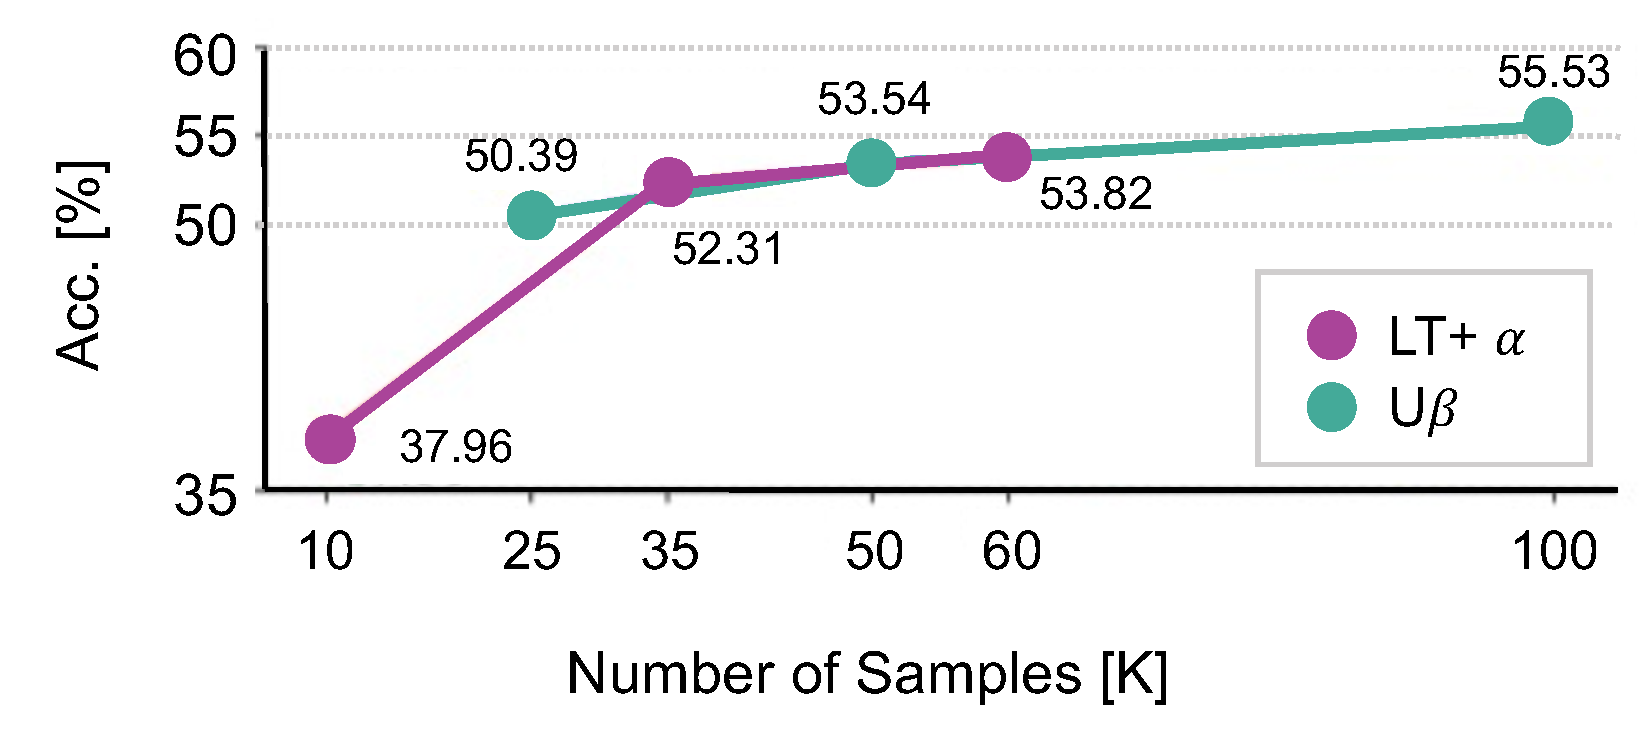
\includegraphics[width=0.95\linewidth]{figures/num_data.pdf}
    \caption{\textbf{Accuracy [\%] (y-axis) vs. number of samples [K] (x-axis).}
    As expected, the performance improves as more synthetic samples are added.
    Additionally, it is improved significantly when the Few class disappears as the number of samples per class increases.}
    \label{fig:alleviate}
\end{figure}



\paragraph{Performance according to the number of synthetic data.}
We explore the performance according to 
% by varying the 
varying number of synthetic data (See \Fref{fig:alleviate}).
We use CIFAR100-LT with the imbalance factor IF=100, \ie, 
% so
the total number of the original samples is 10,847.
%For LT+$\alpha$, we add the synthetic data to all classes equally without care of Many, Medium, and Few classes.
% \wonseok{
For LT+$\alpha$, we uniformly allocate
% incorporate
synthetic data across all classes disregarding the distinction between Many, Medium, and Few classes.
% }
In this case, the absolute difference in sample amount between classes is kept unchanged.
% remains.
%For U$\beta$, we add synthetic data or cut the original samples to be the total number of samples in each class same, \ie, uniformize the data distribution.
% \wonseok{
For U$\beta$, we ensure an equal number of samples in each class by either adding synthetic data or trimming some of the original samples.
% }


% As shown 
In \Fref{fig:alleviate}, the performance is improved as the number of samples increases regardless of the data distribution.
As the quantity of synthetic data increases, accuracies of LT+$\alpha$ and U$\beta$ become quite similar.
%We think that LT+$\alpha$ becomes far from the long-tailed distribution, \ie, the Few class becomes not Few anymore, although the difference in data amount across classes remains in LT+$\alpha$, which reduces the gap between LT+$\alpha$ and U$\beta$.
% 
% \wonseok{
We think that LT+$\alpha$ tends to deviate from the long-tailed distribution as the number
% quantity
of synthetic data increases, \ie, the Few class becomes not Few anymore. Although the disparities 
% variation
in data quantities across classes exist in LT+$\alpha$, this effect diminishes the difference 
% disparity
between LT+$\alpha$ and U$\beta$ with more synthetic data.
% }





\paragraph{Performance according to the quality of synthetic data.}
We evaluate SYNAuG on ImageNet100-LT.
% considering high resolution.
% Since the step value in Stable Diffusion~\cite{rombach2022high} is known to affect the quality of generated images, 
We conduct an ablation study to investigate the impact of data quality of
% different step values
% on
SYNAuG by controlling the diffusion step parameter
% Since the step value in 
of Stable Diffusion~\cite{rombach2022high}, which is known to affect the quality of generated images.
As shown in 
% On the top of
\Fref{fig:imagenet100_lt}-(Top), the generation quality is low when the number of steps is very small, but there is no big difference to the naked eye as it goes up to a certain number.
Figure~\ref{fig:imagenet100_lt}-(Bottom) shows the quantitative results.
% These results lead to quantitative results as well, as shown at the bottom of \Fref{fig:imagenet100_lt}.
Compared to the CE method~\cite{cui2019class} trained on the original long-tailed data, while the accuracy of the Many class is degraded, we achieve large improvement in the Medium, Few, and even All cases
% in all the classes 
regardless of the synthetic image quality.
% Although the accuracy of the Many class is degraded, overall performance, including Medium and Few classes, is drastically improved.
%The results are considerably apart between using synthetic samples with low quality and one with a certain level of quality, but the difference is marginal when the image quality according to the step value exceeds the threshold.
However, there is a certain level of quality that exhibits a surge point in performance.
% The results are 
% considerably different between using synthetic samples with low quality and one with a certain level of quality. 
% However, 
The difference becomes negligible when 
% the image quality according to 
the step value exceeds a certain threshold, \ie, quality.


\begin{figure}[t]
    \begin{subfigure}[c]{0.9\linewidth}
        \centering
        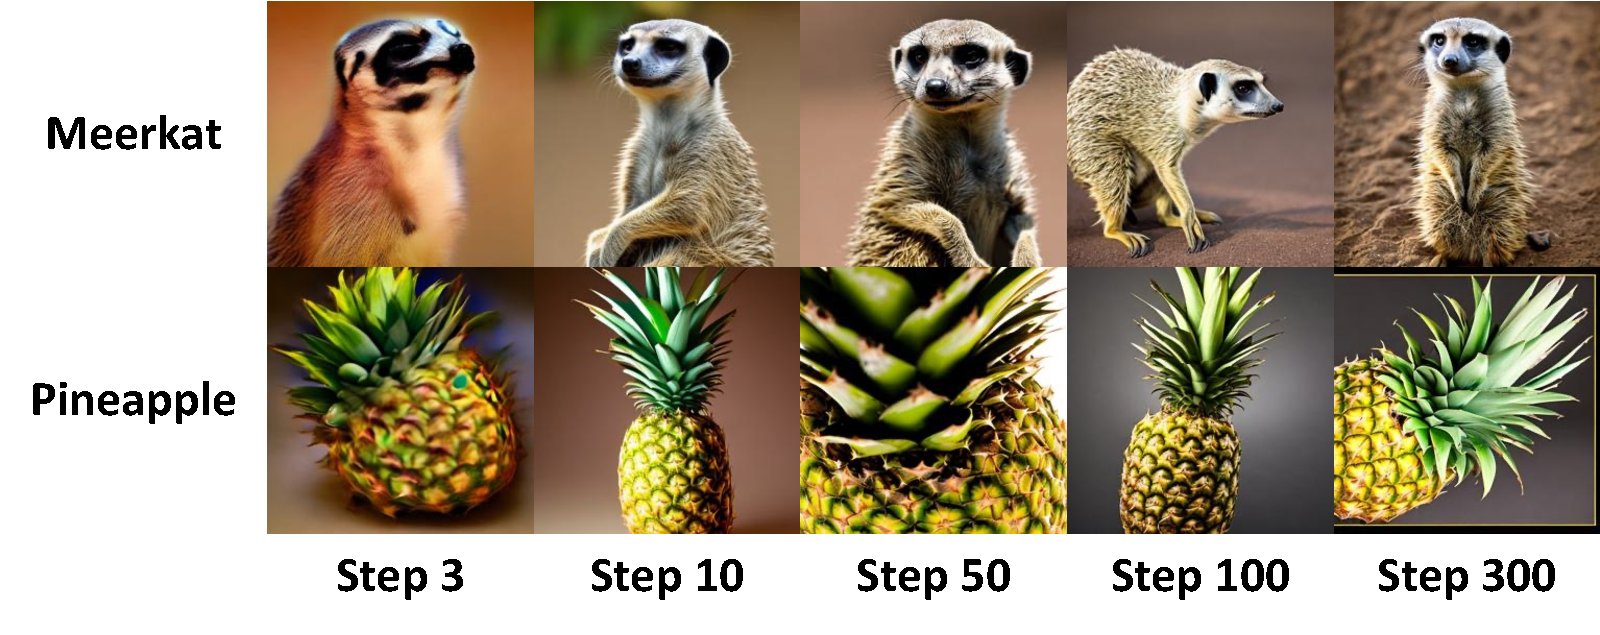
\includegraphics[width=1.0\linewidth]{figures/stepqual_vis.pdf}
    \end{subfigure}
    \centering
    \begin{subtable}[c]{0.9\linewidth}
    \resizebox{1.0\linewidth}{!}{
        \begin{tabular}{@{\,\,\,}lccccc}
            \toprule
            \textbf{Method}  & \textbf{\# step} & \textbf{Many} & \textbf{Medium} & \textbf{Few} & \textbf{All} \\
            \midrule
            CE~\cite{cui2019class}   & & \textbf{61.85} & 15.83 &  0.29 & 32.06 \\
            \cmidrule{1-6}
            \multirow{5}{*}{SYNAuG}
            & 3    & 48.23 & 46.29 & 40.07 & 45.10 \\
            & 10   & 53.89 & \textbf{49.49} & 43.87 & \textbf{49.34} \\
            & 50   & 52.91 & 48.63 & \textbf{45.27} & 49.12 \\
            & 100  & 53.03 & 49.20 & 44.47 & 49.12 \\
            & 300  & 54.11 & 47.71 & 44.73 & 49.06 \\
            \bottomrule 
        \end{tabular}
        }
    \end{subtable}
\caption{\textbf{Ablation study according to sample quality.}
\textbf{(Top)} quality of the generated samples according to the number of steps, \textbf{(Bottom)} long-tailed recognition performance (\%) 
% We report the Top-1 accuracy (\%) 
according to the different times of steps for generating synthetic data, which affects sample quality.
We use ImageNet100-LT with ResNet50.
}
\label{fig:imagenet100_lt}
\end{figure}









\subsection{Model Fairness}\label{sec:fairness}



\begin{figure}[t]
    \centering
    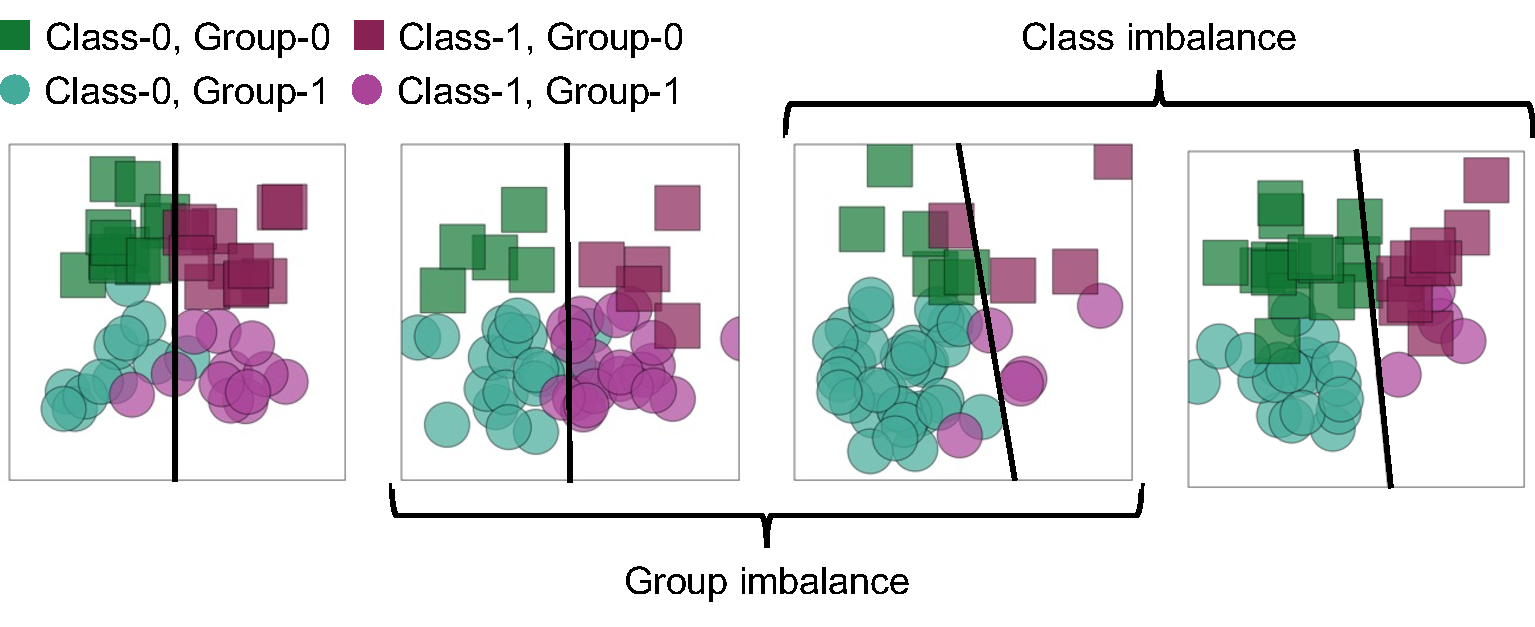
\includegraphics[width=1.0\linewidth]{figures/fairness_toy_exp_2.pdf}
    \caption{\textbf{Influence of the class and group imbalance on classifier during training.} 
    The 2D data are sampled from the normal distributions with four different means and the same covariance. 
    We simulate 4 different experiments with the latent group imbalance (sensitive attributes) by adjusting the number of data in each group.
    The total number of samples is the same.
    We train classifiers for the classes on different imbalance settings and visualize the learned classifiers (bold black lines).
    The fairer the classifiers, the more vertically aligned.
    % When both classes and groups are imbalanced, it yields the most unfair classifier. 
    The classifier trained on the class imbalance is more unfair than the one on the group imbalance.
    % The experiment setting details can be found in the supplementary material.
    }
    \label{fig:fair_toy}
\end{figure}



\begin{table}[]
    \centering
    \begin{subtable}{0.95\linewidth}
        \centering
        \resizebox{\linewidth}{!}{
            \begin{tabular}{lcccc}
            \toprule
            \textbf{Method} & \textbf{Accuracy} & \textbf{DP} & \textbf{ED} & \textbf{EO}\\
            \midrule
            \multicolumn{5}{c}{ResNet18} \\
            \midrule
            % ERM & 93.9 & 0.08174 & 0.0632 & 0.0779\\
            % SYNAuG & 94.0 & 0.06995 & 0.0563 & 0.06825\\
            ERM & 93.9 & 0.0817 & 0.0632 & 0.0779\\
            SYNAuG & \textbf{94.1} & \textbf{0.060} & \textbf{0.0462} & \textbf{0.0434}\\
            \midrule
            \multicolumn{5}{c}{ResNet50} \\
            \midrule
            % ERM & 94.0 & 0.07272 & 0.0585 & 0.07269\\
            % SYNAuG & \textbf{94.1} & \textbf{0.06138} & \textbf{0.04723} & \textbf{0.05885}\\
            ERM & 94.0 & 0.07272 & 0.0585 & 0.07269\\
            SYNAuG & \textbf{94.4} & \textbf{0.05432} & \textbf{0.03936} & \textbf{0.05472}\\
            \bottomrule
           \end{tabular}
        }
    \caption{\textbf{Fairness performance.}}
    \vspace{2mm}
    \label{tab:fairness_1}
    \end{subtable}

    \begin{subtable}{0.95\linewidth}
        \centering
        \resizebox{\linewidth}{!}{
            \begin{tabular}{lcccc}
            \toprule
            \textbf{Method} & \textbf{Accuracy} & \textbf{DP} & \textbf{ED} & \textbf{EO}\\
            \midrule
            ERM & 93.9 & 0.08174 & 0.0632 & 0.0779\\
            + Group-DRO & 93.9 & 0.07266 & 0.05819 & 0.06954\\
            + RS & 93.8 & \textbf{0.0636} & \textbf{0.04663} & \textbf{0.05808} \\
            \midrule
            SYNAuG & \textbf{94.0} & 0.06995 & 0.0563 & 0.06825\\
            + Group-DRO & 93.9 & 0.0711 & 0.05433 & 0.07045\\
            + RS & 93.6 & 0.06786  & 0.06439 & 0.0812 \\
            \bottomrule
           \end{tabular}
        }
       \caption{\textbf{Ablation with other algorithms}}
       \vspace{2mm}
       \label{tab:fairness_2}
   \end{subtable}

    \begin{subtable}{0.95\linewidth}
        \centering
        \resizebox{\linewidth}{!}{
            \begin{tabular}{lcccc}
            \toprule
            \textbf{Method} & \textbf{Accuracy} & \textbf{DP} & \textbf{ED} & \textbf{EO}\\
            \midrule
            ERM & 93.9 & 0.08174 & 0.0632 & 0.0779\\
            + Mixup & 93.9 & 0.07266 & 0.05819 & 0.06954\\
            + CutMix & 94.7 & 0.08265 & 0.06245 & 0.08333\\
            \midrule
            SYNAuG& 94.0 & 0.06995 & 0.0563 & 0.06825\\
            + Mixup & 94.2 & \textbf{0.064} & \textbf{0.03793} & \textbf{0.04658}\\
            + CutMix & \textbf{94.9} & 0.0743 & 0.04745 & 0.06319\\
            \bottomrule
           \end{tabular}
        }
       \caption{\textbf{Augmentation abalation}}
       \vspace{2mm}
       \label{tab:fairness_3}
   \end{subtable}

    \begin{subtable}{0.95\linewidth}
        \centering
        \resizebox{\linewidth}{!}{
            \begin{tabular}{lcccc}
            \toprule
            \textbf{Method} & \textbf{Accuracy} & \textbf{DP} & \textbf{ED} & \textbf{EO}\\
            \midrule
            SYNAuG$^*$ & \textbf{94.0} & 0.07342 & 0.05805 & 0.07253\\ 
            SYNAuG & \textbf{94.0} & \textbf{0.06995} & \textbf{0.0563} & \textbf{0.06825}\\ 
            \bottomrule
            \addlinespace[0.2mm]
            \multicolumn{5}{l}{*Not use the sensitivity attribute}
           \end{tabular}
        }
       \caption{\textbf{Sensitivity abalation}}
       \label{tab:fairness_4}
   \end{subtable}
   
   \caption{\textbf{Fairness performance.} 
   (a) accuracy and model fairness results of our SYNAuG, 
   (b) compatibility with other fairness algorithms, Group-DRO and Re-Sampling (RS), 
   (c) ablation study with data augmentation, Mixup and Cuxmix, 
   and (d) ablation study using the prior about sensitive attribute. \textbf{Bold} means the highest accuracy and the best fairness performance in a table. 
   Higher is better in accuracy, and lower is better in fairness metrics.}
   \label{tab:temps}
\end{table}

Group imbalance stands for the data imbalance between groups, such as ethnicity. 
We empirically observe that the group imbalance with the class imbalance amplifies 
% yields
unfair classifiers, as shown in \Fref{fig:fair_toy}.
The class imbalance affects the unfair classifier more than the group imbalance.
Both class and group imbalance contribute to the unfair classifier.

Model fairness, one of the problems caused by group imbalance, is essential to prevent unexpected social confusion.
Fairness metrics have been proposed to measure the fairness performance of models:
Demographic Parity (DP) $=\max_z|P(y_p{=}1|z) {-} P(y_p{=}1)|$ \cite{10.1145/2783258.2783311},
Equal Opportunity (EO) $=\max_{z_i, z_j, y, y_p}|P_{z_i}(y_p|y) {-} P_{z_j}(y_p|y)|$ \cite{hardt2016equality, jung2022learning},
and Equalized Odds (ED) $=\max_{z, y, y_p}|P(y_p|z, y) {-} P(y_p|y)|$ \cite{hardt2016equality}, where $y_p$ is the prediction, $y$ is the class label, and $z$ is the sensitive attribute.
These metrics are based on the difference in the performance of the learned classifiers depending on groups, \ie, the sensitive attributes.
Lower values of fairness metrics indicate that the model is fairer.


% \begin{table*}[t]
%     \begin{subtable}[b]{0.49\linewidth}
%         \centering
%         \resizebox{\linewidth}{!}{
%             \begin{tabular}{lcccc}
%             \toprule
%             Method & Accuracy & DP & ED & EO \\
%             \midrule
%             % ERM & 93.9 & 0.08174 & 0.0632 & 0.0779\\
%             % SYNAuG$^*$ & \textbf{94.0} & 0.07342 & 0.05805 & 0.07253\\ ICCV 
%             % SYNAuG & \textbf{94.0} & \textbf{0.06995} & \textbf{0.0563} & \textbf{0.06825}\\ ICCB
%             ERM & 93.9 & 0.0817 & 0.0632 & 0.0779\\
%             SYNAuG & \textbf{94.1} & \textbf{0.060} & \textbf{0.0462} & \textbf{0.0434}\\
%             \bottomrule
%            \end{tabular}}
%        \caption{\textbf{Balancing with SYNAuG.}}
%        \label{tab:fair_syn}
%     \end{subtable}
%     \hfill
%     \begin{subtable}[b]{0.49\linewidth}
%         \centering
%         \resizebox{\linewidth}{!}{
%             \begin{tabular}{lcccc}
%             \toprule
%             Method & Accuracy & DP & ED & EO\\
%             \midrule
%             ERM & 93.9 & 0.08174 & 0.0632 & 0.0779\\
%             + Groupp-DRO & 93.9 & 0.07266 & 0.05819 & 0.06954\\
%             + RW & 93.8 & 0.0636 & 0.04663 & 0.05808 \\
%             \midrule
%             SYNAuG & \textbf{94.0} & \textbf{0.06995} & 0.0563 & \textbf{0.06825}\\
%             + Group-DRO & 93.9 & 0.0711 & \textbf{0.05433} & 0.07045\\
%             + RW & 93.6 & 0.06786  & 0.06439 & 0.0812 \\
%             \bottomrule
%            \end{tabular}
%         }
%        \caption{\textbf{Algorithm generalization}}
%        \label{tab:week2}
%    \end{subtable}
   
%     \begin{subtable}[b]{0.49\linewidth}
%         \centering
%         \resizebox{\linewidth}{!}{
%             \begin{tabular}{lcccc}
%             \toprule
%             Method & Accuracy & DP & ED & EO\\
%             \midrule
%             ERM & 93.9 & 0.08174 & 0.0632 & 0.0779\\
%             + Mixup & 93.9 & 0.07266 & 0.05819 & 0.06954\\
%             + CutMix & 94.7 & 0.08265 & 0.06245 & 0.08333\\
%             \midrule
%             SYNAuG& 94.0 & 0.06995 & 0.0563 & 0.06825\\
%             + Mixup & 94.2 & \textbf{0.064} & \textbf{0.03793} & \textbf{0.04658}\\
%             + CutMix & \textbf{94.9} & 0.0743 & 0.04745 & 0.06319\\
%             \bottomrule
%            \end{tabular}
%         }
%        \caption{\textbf{Augmentation generalization}}
%        \label{tab:week2}
%    \end{subtable}
%    \hfill
%    \begin{subtable}[b]{0.49\linewidth}
%         \centering
%         \resizebox{\linewidth}{!}{
%             \begin{tabular}{lcccc}
%             \toprule
%             Method & Accuracy & DP & ED & EO\\
%             \midrule
%             \multicolumn{5}{c}{ResNet18} \\
%             \midrule
%             % ERM & 93.9 & 0.08174 & 0.0632 & 0.0779\\
%             % SYNAuG & 94.0 & 0.06995 & 0.0563 & 0.06825\\
%             ERM & 93.9 & 0.0817 & 0.0632 & 0.0779\\
%             SYNAuG & \textbf{94.1} & \textbf{0.060} & \textbf{0.0462} & \textbf{0.0434}\\
%             \midrule
%             \multicolumn{5}{c}{ResNet50} \\
%             \midrule
%             % ERM & 94.0 & 0.07272 & 0.0585 & 0.07269\\
%             % SYNAuG & \textbf{94.1} & \textbf{0.06138} & \textbf{0.04723} & \textbf{0.05885}\\
%             ERM & 94.0 & 0.07272 & 0.0585 & 0.07269\\
%             SYNAuG & \textbf{94.4} & \textbf{0.05432} & \textbf{0.03936} & \textbf{0.05472}\\
%             \bottomrule
%            \end{tabular}
%         }
%        \caption{\textbf{Architecture generalization.}}
%        \label{tab:week2}
%    \end{subtable}
     
%      \caption{\textbf{Fairness performance.} (a) shows the result of our SYNAuG, (b) the experiments with Group-DRO, (c) the experiments with data augmentation, Mixup and Cuxmix, and (d) experiments with deeper architecture, ResNet50. \textbf{Bold} means the highest accuracy and the best fairness performance in a table. Higher is better in accuracy, and lower is better in fairness metrics.}
%      \label{tab:temps}
%      \vspace{-5mm}
% \end{table*}

\paragraph{Experiments on UTKFace.}
We employ UTKFace~\cite{zhifei2017cvpr} composed of 23,708 images with age, gender, and race labels.
We use race annotation as a sensitive attribute (group label) and gender as the class label.
For SYNAuG, we augment the data to mitigate the class imbalance across the sensitive attribute;
the female and male ratio of each sensitive attribute becomes equal.
%We evaluate the accuracy and fairness metric from the model at the last epoch.
% 바로 뒤에는 fairness metrics 로 쓰셔서 혹시 몰라 적어놓겠습니다.
We evaluate the accuracy and fairness metrics from the model at the last epoch.
Firstly, we validate the effectiveness of SYNAuG in \Tref{tab:fairness_1}.
The result shows that SYNAuG outperforms ERM in accuracy and fairness metrics on both ResNet18 and ResNet50.

\paragraph{Ablation with other algorithms.} 
%In \Tref{tab:fairness_2}, we experiment with the algorithm explaining the sensitive attributes, Group-DRO~\cite{sagawa2019distributionally} and Re-Sampling (RS).
% 바로 위와 같은 이유로 달아 놓겠습니다.
In \Tref{tab:fairness_2}, we evaluate the performance of the two algorithms Group-DRO~\cite{sagawa2019distributionally} and Re-Sampling (RS).
Note that we do not apply Mixup and fine-tuning in this experiment.
Group-DRO and RS improve the fairness metrics of ERM at the same time.
SYNAuG without Group-DRO outperforms the accuracy and two fairness metrics, ED and EO, compared to Group-DRO.
Developing a fairness algorithm with synthetic data might be a promising direction toward a fair model.

\paragraph{Augmentation ablation.} 
In \Tref{tab:fairness_3}, we compare the effect of data augmentations, Mixup~\cite{zhang2017mixup} and CutMix~\cite{yun2019cutmix}.
In this ablation study, we do not apply fine-tuning for clear comparison.
Both augmentations improve the accuracy of ERM; Mixup also works 
% does
in the fairness metrics.
Compared to ERM with Mixup, SYNAuG shows higher accuracy and better fairness metrics.
% EO metric, but underperforms in the other two metrics.
SYNAuG with Mixup outperforms more in accuracy and fairness metrics compared to ERM with Mixup.


\paragraph{No prior of sensitive attribute.}
Labeling sensitive attributes might be expensive.
In this ablation study, we augment the synthetic data to mitigate the class imbalance regardless of sensitive attributes.
We denote this setting as SYNAuG$^*$.
As shown in \Tref{tab:fairness_4}, SYNAuG$^*$ shows better fairness metrics compared to ERM.
However, exploiting the knowledge of sensitive attributes is more effective.

\paragraph{Summary.} 
Class imbalance in fairness can easily cause an unfair model.
This motivates us to balance the class imbalance using synthetic data before tackling fairness directly.
We observe that the synthetic data improves both model accuracy and fairness simultaneously.
The experimental results also demonstrate that SYNAuG is compatible with other training algorithms, data augmentation, and network architecture.




\subsection{Model Robustness to Spurious Correlation}\label{sec:robustness}

A class may include dominant patterns, \ie, spurious correlations.
For example, waterbirds are usually on water rather than land.
It leads DNNs to rely heavily on these spurious features rather than reasoning; thereby, DNNs classify water images as waterbirds regardless of the existence of waterbirds.
This spurious correlation is also caused by data imbalance because fewer waterbirds are located on land.
While spurious correlation occurs naturally, we can mitigate their impact by resolving data imbalance
% generating samples
similar to model fairness.
% long-tailed distribution.
% not to be correlated with spurious features.
We demonstrate whether SYNAuG can mitigate the data imbalance problem of spurious correlations.

% % which can drift the model to cause bias or misconception, \ie, spurious correlations.
% % DNNs heavily rely on these spurious features rather than reasoning, because these features are easy to learn.
% For example, DNNs can classify the empty road image as the models are trained with lots of car images on a road that usually takes a much larger area than that of cars.
% % spurious corr하고 imbalance하고 연관
% Although spurious correlations caaturally, we can mitigate their impact by generating samples in rare classes that are not correlated with the sensitive attributes.
% % to generate rare samples using diffusion models.
% We demonstrate whether SYNAuG can mitigate the data imbalance problem, which causes spurious correlations.


\begin{table}
    \centering
        \resizebox{0.9\linewidth}{!}{
            \begin{tabular}{lcc}
            \toprule
            \multirow{2}[2]{*}{\textbf{Method}} & \multicolumn{2}{c}{\textbf{Waterbirds}}\\
            \cmidrule{2-3}
            & \textbf{Worst} & \textbf{Mean}\\
            \midrule
            ERM & 72.6 & 97.3\\
            JTT$_\texttt{ ICML'21}$~\cite{liu2021just} & 86.7 & 93.3 \\
            Group-DRO$_\texttt{ ICLR'20}$~\cite{sagawa2019distributionally} & 91.4 & 93.5\\
            SUBG$_\texttt{ ICML'20}$~\cite{sagawa2020investigation} & 89.1$_{\pm 1.1}$ & -\\
            SSA$_\texttt{ ICLR'22}$~\cite{nam2022spread} & 89.0$_{\pm 0.55}$ & 92.2$_{\pm 0.87}$\\
            \midrule
            BaseModel & 73.7$_{\pm 3.04}$ & 90.4$_{\pm 0.21}$\\
            % BaseModel$_{\text{web}}$ & 80.1$_{\pm 1.95}$ & 94.3$_{\pm 0.38}$\\
            SYNAuG & 79.9$_{\pm 2.22}$ & 91.52$_{\pm 0.98}$\\
            \midrule
            % DFR$^{\text{Tr}}_{\text{Tr}}$$_\texttt{ ICLR'23}$~\cite{kirichenko2023last} & 89.2$_{\pm 1.91}$ & 94.2$_{\pm 0.74}$\\
            % % DFR$^{\text{Tr-web}}_{\text{Tr}}$ & 92.8$_{\pm 1.13}$ & 96.0$_{\pm 0.55}$\\
            % SYNAuG & 90.3$_{\pm 0.81}$ & 93.7$_{\pm 0.24}$\\
            % SYNAuG & 79.8$_{\pm }$ & 92.4$_{\pm }$\\
            % \midrule
            DFR$^{\text{Tr}}_{\text{Val}}$$_\texttt{ ICLR'23}$~\cite{kirichenko2023last} & 91.2$_{\pm 1.92}$ & 93.1$_{\pm 0.91}$\\
            % DFR$^{\text{Tr-web}}_{\text{Val}}$ & 93.9$_{\pm 0.60}$ & 95.4$_{\pm 0.40}$\\
            SYNAuG (re-train) & 92.9$_{\pm 0.45}$ & 93.6$_{\pm 0.35}$\\
            SYNAuG (fine-tuning) & 93.2$_{\pm 0.42}$ & 94.8$_{\pm 0.11}$\\
            \bottomrule
           \end{tabular}}
       \caption{\textbf{Robustness to spurious correlation on Waterbirds.} 
       SYNAuG outperforms DFR consistently in worst-group accuracy.}\vspace{4mm}
       \label{tab:robustness}
\end{table}

\paragraph{Experiments.} 
We use Waterbirds dataset~\cite{sagawa2019distributionally}, which is a synthetic dataset created by combining images of birds from the CUB dataset~\cite{WelinderEtal2010} with backgrounds.
%The seabirds and waterfowl are grouped in a waterbird, and the other birds in a landbird.
The birds are grouped into two categories: waterbirds, which include seabirds and waterfowl, and landbirds.
Land and water background are spurious features.
Let $G_{\text{background}}^{\text{class}}$ be the class with the background, \eg, $G_{\text{water}}^{\text{landbird}}$ is the landbird with water background.
% where the class is waterbirds or landbirds, and the background is land or water.
% Let $G_1, G_2, G_3$, and $G_4$ be landbird with land background, landbird with water background, waterbird on land background, and waterbird with water background, respectively.
In the Waterbirds dataset, $G_{\text{land}}^{\text{landbird}}$ has more samples than $G_{\text{water}}^{\text{landbird}}$, and $G_{\text{water}}^{\text{waterbird}}$ has more samples than $G_{\text{land}}^{\text{waterbird}}$.
We generate the samples to match the number of samples such as $|G_{\text{land}}^{\text{landbird}}| = |G_{\text{water}}^{\text{landbird}}|$ and $|G_{\text{water}}^{\text{waterbird}}| = |G_{\text{land}}^{\text{waterbird}}|$.
% $G_1$ and $G_2$, and $G_3$ and $G_4$.
% Following Sagawa~\etal\cite{sagawa2019distributionally}, we evaluate algorithms using the minimum group accuracy and the average (in-distribution) accuracy, denoted as Worst and Mean, respectively.
We report the result over 5 independent runs using the code from DFR~\cite{kirichenko2023last}.
We reproduce the BaseModel and DFR and report the performance at the last epoch\footnote{\url{https://github.com/PolinaKirichenko/deep_feature_reweighting}}.

In \Tref{tab:robustness}, our SYNAuG generates samples not to be correlated with spurious features, which
improves the performance in BaseModel both on worst and mean accuracies.
When applying DFR, the synthetic data can increase the worst and mean accuracy consistently.
% In addition, w
We also observe that fine-tuning is more effective 
% shows better performance
compared to re-train, which is consistent with \Tref{tab:ablation}.
% It indicates 
The overall results demonstrate that the synthetic data from the generative model can be exploited to mitigate the spurious correlation.



%-------------------------------------------------
%-------------------------------------------------
\section{Conclusion and Discussion}\label{sec:conclusion}

We propose SYNAuG which deals with long-tailed recognition, model fairness, and robustness to spurious correlations as data imbalance problems.
% SYNAuG consists of three stages: (1) uniformization of training data, (2) model training, and (3) classifier fine-tuning.
The development process of the machine learning model 
% development process 
can be roughly divided into 
data curation, model training, and model management.
Since the data comes first in the process,
% among these parts,
a flaw in the dataset affects the subsequent phases; thus, it is crucial.
% Therefore, careless handling of data can cause social and ethical confusion.
Our study suggests the importance of controlling imbalance from the data perspective.
We believe that taking the controllability of data is a promising research direction to resolve the early bottleneck in machine learning model development. 
While we focus on the data perspective, improving the model in multiple views is necessary for effective solutions to data imbalance.
We conclude our work with the following discussions.

\paragraph{Other perspectives.}
We have suggested the usage of synthetic data from pre-trained generative models as a new data perspective baseline for the data imbalance problem, but there may be other perspectives.
% to address the data imbalance.
We observed a gradual performance decline when substituting real data with synthetic data, suggesting the potential need for domain adaptation.
There could be future research directions, \eg, more sophisticated data augmentation, automated data curation, transfer learning, the usage of differentiability of the generative models, and comprehending taxonomies across classes.
% In addition, studying the contamination of real data by synthetic data would provide guidelines about how to exploit the generated data.
While we emphasize that our work suggests a promising way to redraw the direction to overcome the data imbalance problems in the data perspective, more interesting future work will come with integrating multiple levels.

% \paragraph{Implications of synthetic data supplements.}
% As generative models have a huge impact on the public, anyone can upload the result on the web without indicating whether it is synthetic or not.
% Not only are humans exposed to synthetic information, but DNNs can also be exposed to this information.
% Although we focus on the supplements of original data with synthetic data in this work, studying the contamination of real data by synthetic data would provide guidelines about how to exploit the generated data.

\paragraph{Limitations of using generative models.}
The generation of synthetic data demands additional time and computational resources. 
While the curation of a real dataset requires enormous time, human, and financial resources, the process of generating synthetic data becomes increasingly challenging as the volume of data needed increases.
Also, the quality of the synthesized data varies depending on factors such as the prompt, guidance level, and step value of the diffusion model, impacting the overall performance of the model. 
However, since generative models have been continuously developed in terms of sample quality, time efficiency, and controllability,
we believe that exploiting generation models as a data source is a promising research direction as the performance of generation models is improved.

% \paragraph{Social Impact.}




%%%%%%%%% REFERENCES
{\small
\bibliographystyle{ieee_fullname}
\bibliography{egbib}
}

\end{document}


Deep neural networks (DNNs) have achieved strong performance on visual tasks.
The outstanding performance has been demonstrated by training a model with abundant and diverse labeled data
% ,~\eg,
~\cite{deng2009imagenet, lin2014microsoft}.
Despite the importance of data, machine learning researchers have focused mainly on the model and algorithms~\cite{sambasivan2021everyone}.
We should care about the data for training DNNs because unexpected influences can occur by data.
% and there is a lack of data debugging tools.
% We should first curate the dataset well for training the model because unexpected cascades can occur depending on the curated data~\cite{sambasivan2021everyone}.
% However, such abundant and well-curated labeled data are not available.
% The state-of-the-art DNNs suffer from much lower performance in certain types of classes or groups because of data imbalance.

We commonly encounter data imbalance problems categorized into \emph{class} or \emph{group} imbalance problems.
% The data imbalance problems we commonly encounter are mainly categorized into \emph{class} or \emph{group} imbalance problems.
Class imbalance means different data amounts in the classes.
Suppose that we collect animal images on the internet.
Images of rare animals may be found on search engines less than cats or dogs because of human bias for uploading their photograph~\footnote{For example, the number of search results of Tarsier is about 102 times less than Maltese in Google search engine.}.
Group imbalance, on the other hand, stands for different data amounts in the groups.
We may collect data depending on our environments, including preferences, country, and cultural backgrounds.
Suppose we collect a picture of human hands; then, the skin tones can be biased.
% The curator also may collect data depending on their environments\footnote{The skin tones of hands are imbalance~\cite{grady2022pressurevision}.}, such as preference, country, and cultural backgrounds, which implies the \emph{group imbalance problem}.
If we do not care about these biases, the collected dataset becomes imbalanced in terms of classes~\cite{cui2019class,zhang2023deep}, groups~\cite{whang2021responsible}, or both.
% These biases lead the collected dataset to be imbalanced in terms of classes~\cite{cui2019class,zhang2023deep} and groups~\cite{whang2021responsible}.
With such a dataset and the standard supervised learning algorithms based on empirical risk minimization (ERM) principle~\cite{vapnik1999nature}, the classifier will be trained to 
% will
be biased to majority classes~\cite{geirhos2020shortcut}.
Since these problems yield not only substantial performance degradation but also social or ethical issues with biases, researchers have independently developed various algorithms~\cite{arjovsky2019invariant,bahng2020learning,sagawa2019distributionally,teney2020unshuffling,tartaglione2021end, lee2021learning,LfF,liu2021just, kim2022learning,yao2022improving,hwang2022selecmix,kirichenko2023last,cao2019learning,ren2020balanced,samuel2021distributional, shen2016relay,park2022majority,kim2020m2m,liu2019large,zhang2022correct} to overcome these respective problems.

\begin{figure}[t]
    \centering
    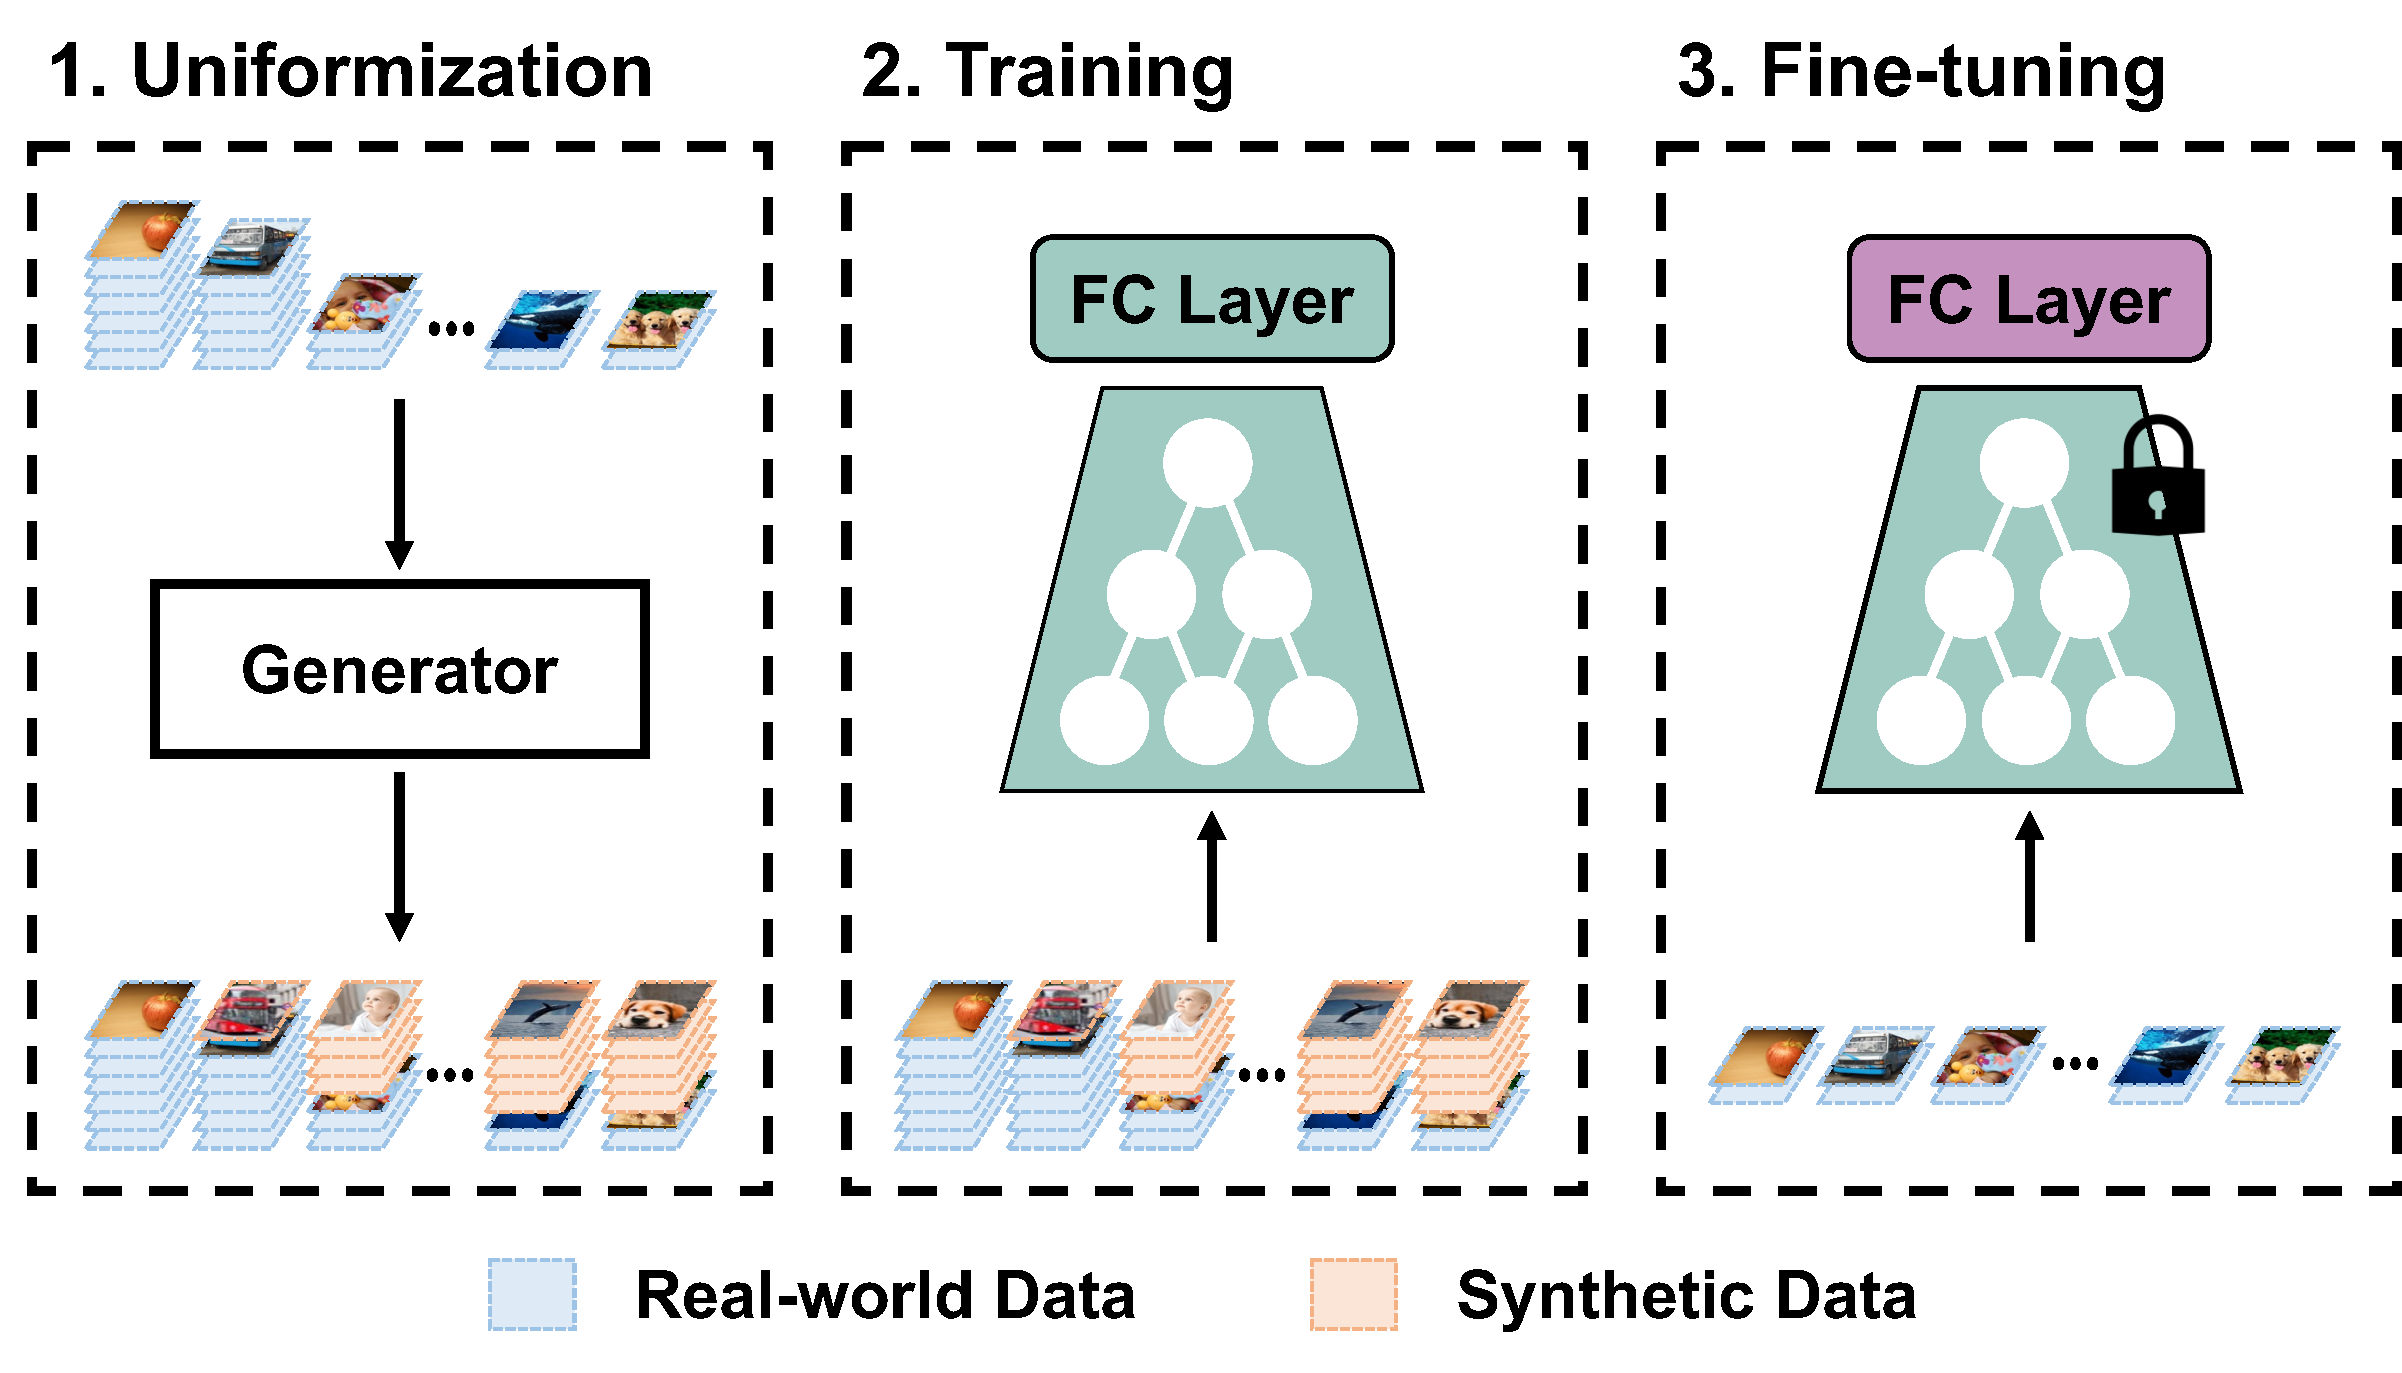
\includegraphics[width=1.0\linewidth]{figures/final.pdf}
    \caption{\textbf{Overview of SYNAuG process.}
    % \textcolor{realblue}{\textbf{legenBlue}} is the real-world data, and \textcolor{synorange}{\textbf{orange}} is the synthetic data.
    Given the imbalanced real-world data with the class labels, we first uniformize the imbalanced real data distribution by generating the synthetic samples that are conditioned on the class label.
    Second, we train a model with the uniformized training data.
    Finally, we fine-tune the last layer with the uniformly subsampled real-world data.}
    \label{fig:overview}
\end{figure}

In this work, we first uniformize the number of samples in each class using the recent text-to-image generative models before applying off-the-shelf task-specific algorithms.
% This takes a different direction, unlike the prior methods.
The prior studies 
% have reported improved performance over the state-of-the-art in their respective tasks.
% However, they use
work the limited, fixed, and bounded original dataset without adding more additional data and mainly focus on algorithmic approaches, such as reweighting~\cite{cao2019learning,ren2020balanced,samuel2021distributional,huang2019deep, ben2009robust, sagawa2019distributionally, jung2023reweighting}, resampling~\cite{shen2016relay,park2022majority,kim2020m2m,liu2019large, kamiran2012data, idrissi2022simple, roh2020fairbatch}, or augmentation~\cite{chuang2021fair, kim2020m2m, park2022majority}.
In contrast to the prior arts, we go beyond the fixed original dataset by exploiting
% , we exploit 
the generative diffusion models to synthesize data, which have recently shown potential as synthetic training data generation~\cite{poole2023dreamfusion, raj2023dreambooth3d, chen2023fantasia3d,trabucco2023effective, he2022synthetic, azizi2023synthetic}.
This allows us to tackle the fundamental bottleneck of data imbalance, \ie, data, rather than indirect ways of tackling learning algorithms or architectures.
It is a more natural way than restricting training data to the fixed dataset as in the prior arts.
% , which would be unnecessary in the generative model era.
% In the generative model era, we argue that restricting training data to the fixed dataset is impractical.
% Furthermore, data imbalance problems should be tackled from the data level before deploying algorithmic approaches.
% so that the practitioners take the controllability of data to mitigate and stabilize the base conditions of datasets.

As shown in \Fref{fig:overview}, we propose SYNAuG, exploiting the generative diffusion model to augment and make the original data distribution to be uniform distribution, \ie, uniformization.
% uniformize the original training data.
% , motivated by recent class imbalance approaches~\cite{kim2020m2m,he2022synthetic,kirichenko2023last}.
After training on the uniformized data composed of the original and synthetic data, we found that it is effective to use simple fine-tuning of the last layer with uniformly sub-sampled original data.
% after pretraining on the mixed dataset.
This outperforms the other strong baselines, including the baseline using the additional external web data as well as the competing methods on the long-tailed recognition benchmark, CIFAR100-LT, and the fairness benchmark, UTKFace.
In addition, we demonstrate the effectiveness of our method for improving the robustness of the classifier to spurious correlation.
We summarize our contributions as follows:
\begin{itemize}
    \item Proposing SYNAuG that uniformizes the given data distribution with synthetic data, beyond the given datasets;\vspace{-1mm}
    % not restricted to the given datasets;
    \item Demonstrating the effectiveness of SYNAuG on three distinctive data imbalance tasks: long-tailed recognition, model fairness, and robustness to spurious correlation;
    \vspace{-1mm}
    \item Reporting the observation of the importance of a few original samples when we use synthetic data together.
\end{itemize}






% \paragraph{Data Imbalance Problems.}
% In the real world, dogs and cats outnumber rare animals, and this characteristic of nature is reflected in the curation of data.
% These data imbalance problems can cause poor generalization and many issues in finance, healthcare, and autonomous driving.
% In this paper, we tackle long-tailed recognition, fairness, and model robustness to spurious correlation, which are related closly from the data imbalacne perspective.

% Imbalance in data
Data imbalance can lead to
% cause poor
suboptimal generalization and many challenges
% issues
in practical application scenarios, \eg, finance, healthcare, and autonomous driving.
The data imbalance problem is a common source of different imbalance sub-problems: long-tailed recognition, model fairness, and model robustness to spurious correlation.
% This work is related to the data imbalance problem, and 
We brief the related work on the associated sub-problems and on using synthetic data for machine learning tasks.
% review its associated sub-problems and using synthetic data.
% : class imbalance (long-tail), fairness, and spurious correlation.
% In this paper, we tackle which are related closly from the data imbalacne perspective.



% \begin{wrapfigure}{r}{0.45\linewidth}
%     \centering
%     \vspace{-6mm}
%     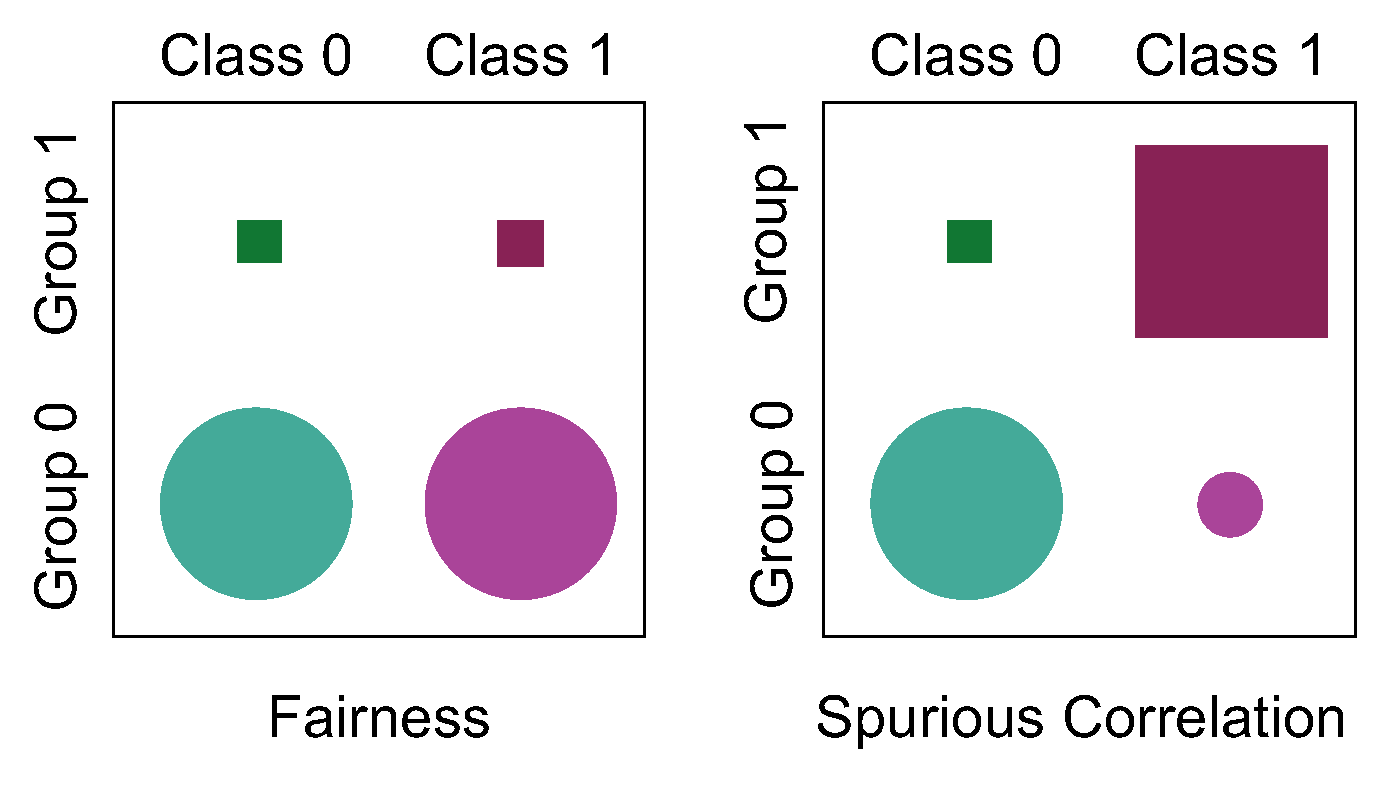
\includegraphics[width=1.0\linewidth]{figures/group_imbalance_teaser.pdf}
%     \caption{\textbf{Overview of fairness and spurious correlation from the data perspective.}
%     The size of a shape represents the amount of data. The same shape stands for the same group, and the same color for the same class.\vspace{-3mm}}
%     % 
%     \label{fig:group_imbalance_teatures}
% \end{wrapfigure}

% It is well-known that long-tailed recognition~\cite{cui2019class,zhang2023deep}, where their training data follow Pareto distribution, is one of the class imbalance problems.
% Long-tailed distribution, \ie, Pareto distribution, is natural in the real world, which has a class imbalance.
% Dogs and cats outnumber rare animals, and this characteristic of nature is reflected in the curation of data.


% (see \Fref{fig:group_imbalance_teatures}).

% Model robustness is related to spurious correlations that some classes appear with certain patterns, \ie, spurious or shortcut features~\cite{geirhos2020shortcut, scimeca2022iclr, kirichenko2023last}.

% for deep neural networks 

% Since the long-tail distribution, model robustness, and model fairness are related closely from the data imbalance perspective, we handle these three data imbalance problems.



\paragraph{Long-tailed recognition.}
Long-tailed distribution is inherent to the real world~\cite{cui2019class,zhang2023deep}.
There are two main streams in the realm of re-balancing classes, including re-sampling~\cite{shen2016relay,park2022majority,kim2020m2m,liu2019large} and re-weighting~\cite{he2009learning,samuel2021distributional, cao2019learning, ren2020balanced, lin2017focal, ryou2019anchor, cui2019class}.
The re-weighting methods share a similar mechanism to weighting minority classes inverse-proportionally to the number of instances. 
% less frequent class by the inverse of frequency~\cite{he2009learning, cui2019class}.
The re-sampling methods weight the samples in minority classes by more frequently sampling with replacement so that the training model can see the uniform number of samples across classes.

There are other approaches 
% to tackle the problem
by designing loss functions.
Ryou~\etal\cite{ryou2019anchor} and Lin~\etal\cite{lin2017focal} 
% design loss functions that 
induce adaptive re-weighting effects during training.
The others take into account margin~\cite{cao2019learning} or balance of softmax~\cite{ren2020balanced} in the loss design.
% Also, there are other approaches to take into account other factors in the loss design: margin~\cite{cao2019learning} or balance of softmax~\cite{ren2020balanced}.
Wang~\etal\cite{wang2021longtailed} take a completely different approach; model selection given diversely pre-trained classifiers.
In addition, Ye-Bin~\etal\cite{yebin2023textmania} propose
% proposes
TextManiA, visual feature augmentation for sparse samples, which shows improved performance in long-tailed distribution.


\paragraph{Model fairness.} 
In fairness~\cite{narayanan2018translation, hardt2016equality, 10.1145/2783258.2783311}, researchers have tackled the issue of model bias, where accuracy varies based on 
% the unfairness that the model accuracy is different depending on
sensitive attributes such as race, age, and ethnicity.
Model fairness is also related to data imbalance because the number of samples of some sensitive groups is lower than that of the major groups.
Fairness has predominantly been tackled using loss weighting and batch sampling.
A loss weighting algorithm~\cite{jung2023reweighting} proposes fairness optimization, where they minimize the worst-case loss of the group by adaptively weighting losses.
% during training.
Batch sampling approaches~\cite{kamiran2012data, roh2020fairbatch} take an adaptive sampling strategy by considering sensitive information rather than uniform sampling.
Zeng~\etal\cite{zeng2022fair} take a post-calibration approach after training
% with the above existing method
to calibrate the classifiers.


% arjovsky2019invariant,bahng2020learning,sagawa2019distributionally,teney2020unshuffling,tartaglione2021end, lee2021learning,LfF,liu2021just, kim2022learning,yao2022improving,hwang2022selecmix,kirichenko2023last,cao2019learning,ren2020balanced,samuel2021distributional, shen2016relay,park2022majority,kim2020m2m,liu2019large
\paragraph{Spurious correlation.}
% While the spurious correlation problem shares similarities with fairness, it 
The spurious correlation problem is related to the robustness of models against misleading correlations.
DNNs are susceptible to falling into shortcuts that capture the most frequently observed patterns in a class regardless of true causality;
it is called spurious correlation or shortcut problems~\cite{geirhos2020shortcut, scimeca2022iclr, kirichenko2023last}.
It is never desirable to rely on spurious features that degrade the generalizability of DNNs~\cite{sagawa2019distributionally, liu2015deep}.
The spurious correlation problem is also dealt with similar approaches to the above two tasks: weighting~\cite{sagawa2019distributionally,LfF,kim2022learning}, sampling~\cite{idrissi2022simple, sagawa2020investigation}, augmentation~\cite{lee2021learning,yao2022improving,hwang2022selecmix}, and post-calibration~\cite{liu2021just, kirichenko2023last, lee2022surgical}.


\paragraph{Summary of data imbalance problems.}
While researchers have developed algorithms for each task separately, three different tasks sourced from data imbalance have mainly been tackled in the shared perspective, \ie, 
% re-balancing; 
up-weight loss values or sampling probabilities of minor groups using group or sensitive information.
However, they have focused only on algorithmic parts by limiting their methods to exploit the given imbalance dataset, where the inherent imbalance still remains.

In this work, we shed light on the overlooked convention to go beyond the given bounded dataset.
We exploit the synthetic data from the generative foundation models~\cite{rombach2022high, saharia2022photorealistic, nichol2021glide} to take flexibility and controllability so that we can populate the long-tailed training data distribution to become a uniform distribution, which mitigates the imbalance problem itself.
We observe that this simple correction of class distribution with synthetic data can significantly improve the worst-case accuracy and fairness of DNNs.
To our best knowledge, our work is the first work that demonstrates improved or competitive performance with generated synthetic data for both class imbalance and fairness tasks.

\paragraph{Using synthetic data in machine learning tasks.}
To overcome the lack of data or sensitive issues of data, \eg, licensing and privacy concerns, recent approaches have started to leverage synthetic data for their tasks of interest:
classification~\cite{antoniou2017data, tran2017bayesian}, segmentation~\cite{sandfort2019data, zhang2021datasetgan}, re-identification~\cite{zheng2017unlabeled}, motion estimation~\cite{dosovitskiy2015flownet, mayer2016large, sun2021autoflow, han2022realflow, oh2018learning}, computational photography~\cite{pan2021dual}, and representation learning~\cite{jahanian2021generative}.
Recently, deep generative models~\cite{rombach2022high, saharia2022photorealistic, nichol2021glide} have shown promising results in generating realistic and high-quality samples, stemming from the goal of modeling the real data distribution.
In particular, the image generation conditioned on text provides great controllability and flexibility, which has the potential to be used for a variety of tasks, such as 3D reconstruction~\cite{poole2023dreamfusion, raj2023dreambooth3d, chen2023fantasia3d} and image recognition~\cite{trabucco2023effective, he2022synthetic, azizi2023synthetic}.
In this work, we explore the use of a pre-trained foundation diffusion model to mitigate data imbalance problems.





We live in an era of data floods, and deep neural networks play a pivotal role in this moment.
Natural data inherently exhibits several challenges such as long-tailed distribution and model fairness, where data imbalance is at the center of fundamental issues.
This imbalance poses a risk of deep neural networks producing biased predictions, leading to potentially severe ethical and social problems.
To address these problems, we leverage the recent generative models advanced in generating high-quality images.
In this work, we propose SYNAuG, which utilizes synthetic data to uniformize the given imbalance distribution followed by a simple post-calibration step considering the domain gap between real and synthetic data.
This straightforward approach yields impressive performance on datasets for distinctive data imbalance problems such as CIFAR100-LT, ImageNet100-LT, UTKFace, and Waterbirds, surpassing the performance of existing task-specific methods.
While we do not claim that our approach serves as a complete solution to the problem of data imbalance, we argue that supplementing the existing data with synthetic data proves to be an effective and crucial step in addressing data imbalance concerns.


We first present our motivation for using synthetic data to address data imbalance problems based on experimental findings (\Sref{sec:2.1}).
Building on these empirical insights, we propose to exploit the synthetic data (SYNAuG) as a means to uniformize the given training data distribution 
% of the given training data
(\Sref{sec:2.2}).
% Note that we do not advocate that SYNAuG is a solution for the data imbalance problem, but it provides a novel perspective from a data point of view.

\begin{figure}
    \centering
        \begin{subfigure}[b]{0.9\linewidth}
        \centering
        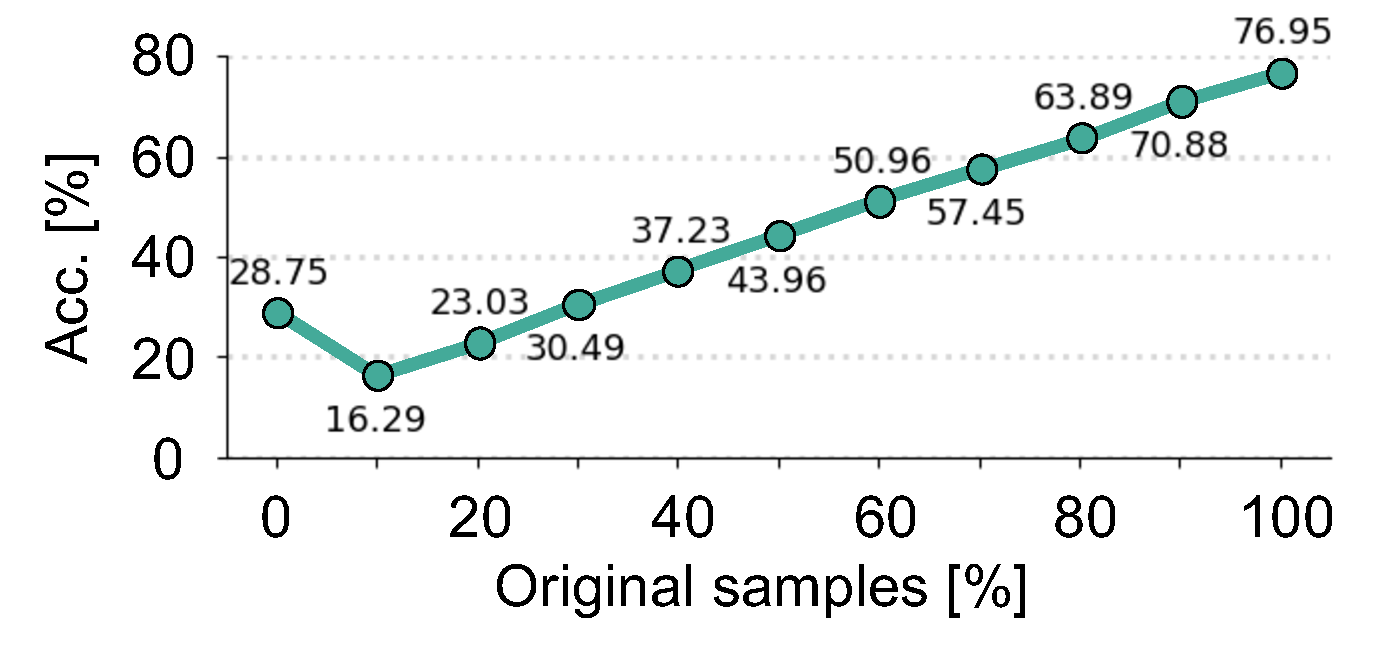
\includegraphics[width=1.0\linewidth]{figures/example1.pdf}
        \caption{Class-wise replacement}
        \label{fig:classwise}
    \end{subfigure}
    \centering
        \begin{subfigure}[b]{0.9\linewidth}
        \centering
        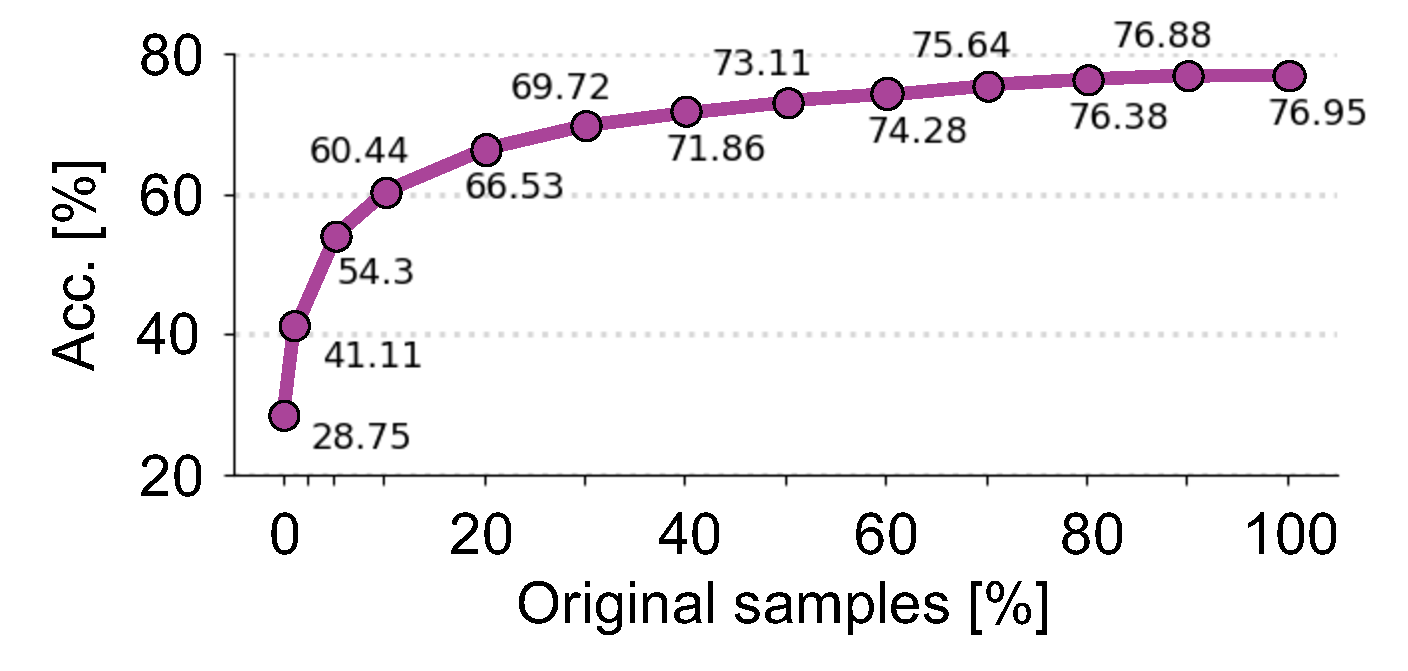
\includegraphics[width=1.0\linewidth]{figures/example2.pdf}
        \caption{Instance-wise replacement}
        \label{fig:instwise}
    \end{subfigure}    
    \caption{\textbf{Replacement test.} 
    To investigate the effect on model performance when using original and synthetic data together, we replace the original data with synthetic ones in two ways: (a) class-wise and (b) the same ratio of instances across all classes.
    We use CIFAR100, which has 500 samples per class and 100 classes.
    }
    \label{fig:abl_ratio}
\end{figure}

\subsection{Motivations}\label{sec:2.1}
During training, we consider how to curate the data, train the model, and evaluate it.
As aforementioned, prior methods addressing data imbalance problems have explored in various ways, including data re-sampling, loss function design, and model architecture.
Instead, 
% As the first step, data curation significantly affects the training and the subsequent evaluation.
we emphasize the importance of data curation and the controllability of data, as data curation significantly affects the training and the subsequent evaluation despite its position as the first step.
% In this work, we propose to utilize the power of the recent text-to-image generative model, which provides controllability in generating synthetic samples.

Before incorporating synthetic data into our proposed method, we delve into the influence of training with synthetic and original data together.
We establish two settings by controlling the ratio of original and synthetic data.
We use the generated images from the Stable Diffusion~\cite{rombach2022high} for synthetic data.
In the \textbf{first setting}, we take an extreme approach by replacing whole original data belonging to specific classes with synthetic data.
It means that certain classes have no real samples but only synthetic samples.
% , and this setting is an extreme case of data imbalance.
In the \textbf{second setting}, we uniformly replace the original data with synthetic data, which means all classes have the same ratio of original and synthetic data.
This approach ensures that every class at least has a few original data.
The significance of original samples becomes apparent through observing the performance change.

% Figure~\ref{fig:abl_ratio} shows t
The results of the two settings are in \Fref{fig:abl_ratio}.
The first setting shows the linear performance degradation as the number of classes with no original data increases (See \Fref{fig:classwise}).
However, the second setting shows the log-like performance degradation as more original data are replaced with synthetic data uniformly (See \Fref{fig:instwise}).
We achieve 41.11\% when using 1\% of real data in the second setting, which is similar to the result of 43.96\% when using 50\% of real data in the first setting.
% The performance of 1\% of real data in the second setting is 41.11\%, which is similar to the performance of 50\% of real data in the first setting, 43.96\%.
%It indicates that few original samples might be needed. and the domain gap might exist despite high-quality synthetic data.
% 어감이 few original samples 이 앵커 역할을 한다는거면 조금 더 강조를 해야할수도..
The results suggest that at least a few original samples are necessary as an anchor, as
% while
the domain gap may still exist even with high-quality synthetic data.
% In addition, the performance difference between 100\% and $n$\% accuracies in \Fref{fig:instwise} would represent the existence of the domain gap between real and synthetic data.

\begin{figure}
    \centering
        \begin{subtable}[c]{0.3\linewidth}
        \centering
        \resizebox{1.0\linewidth}{!}{
            \begin{tabular}{cc}
                \toprule
                & \textbf{Accuracy} \\ 
                \midrule
                Real  & 77.76 \\
                Syn.  & 70.56 \\
                \cmidrule{1-2}
                Total & 74.16 \\
                \bottomrule 
            \end{tabular}
        }
        \caption{Binary domain classification}    
        \label{fig:domain_cls}
    \end{subtable}
    \hspace{8mm}
    \centering
        \begin{subfigure}[c]{0.5\linewidth}
        \centering
        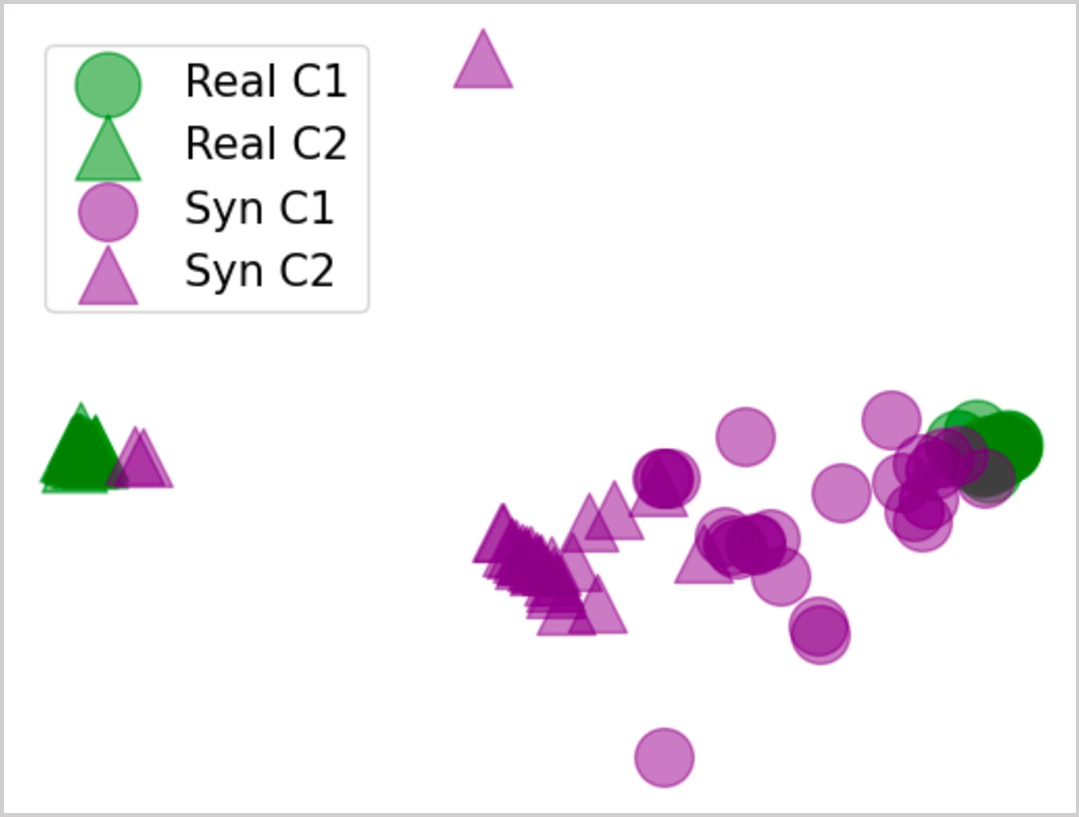
\includegraphics[width=1.0\linewidth]{figures/domain_gap.pdf}
        \caption{Feature visualization}
        \label{fig:domain_feat}
    \end{subfigure}    
    \caption{\textbf{Domain gap between real and synthetic data.} 
    We test the domain gap empirically with (a) binary domain classification and (b) feature visualization.
    For binary classification, we use 2.5k samples for each real and synthetic domain and train only one fully-connected layer with the extracted features.
    For visualization, the features are extracted from the pre-trained model on CIFAR100.
    % , a total of 5k samples.
    % We first train the model with real samples (CIFAR100) and re-train the last layer from scratch to classify the given samples as real or synthetic. 
    % For re-training, we use 2.5k samples for each real and synthetic domain, a total of 5k samples.
    % The features are extracted before the last layer.
    C1 and C2 denote different classes.
    }
    \label{fig:domain}
\end{figure}

To check the presence of a domain gap, we conduct domain classification and visualization of the features from both real and synthetic data (See \Fref{fig:domain}).
As shown in \Fref{fig:domain_cls}, the classification performance is 74.16\%.
This indicates the existence of a domain gap, considering that 50\% means no domain gap.
As shown in \Fref{fig:domain_feat}, the features of Syn C2 are more closer to Syn C1 rather than Real C2.
% the features of synthetic data in class 1 (Syn C1) are closer than features of real data. 
% \wonseok{As shown in \Fref{fig:domain_feat}, the features of synthetic data are more tightly clustered than the features of real data. }
This observation provides empirical evidence of a domain gap existing between real and synthetic data.

% If there is no domain gap between real and synthetic data, the domain classifier would be incapable of distinguishing between samples, yielding an accuracy of 50\%.
% However, as depicted in Figure \ref{fig:domain_cls}, the obtained accuracy of 74.16\% indicates a discernible domain gap.
% Visualization result depicted in \Fref{fig:domain_feat} reveals that some of the synthetic samples are distant from their corresponding real samples within the same class.
% This observation also provides empirical evidence of a domain gap existing between real and synthetic data.

In summary, (1) at least, a few real samples are important when we supplement the real samples with the synthetic samples,
(2) synthetic samples are still insufficient to fully replace the original samples, although the deep generative models show impressive performance,
thus, (3) there might be additional room for improvement due to the domain gap between the original and the synthetic data.
It is desirable that the remaining original samples serve as an anchor role, and synthetic data support and populate the insufficient samples.

% While the first case shows the linear performance degradation as shown in \Fref{fig:classwise}, the second case shows the performance degradation alleviate rather than the first case as shown in \Fref{fig:instwise}.
% Interestingly, the performance of 1\% of original data in the second case is similar to the performance of 50\% of original data in the first case.
% In addition, the performance difference between 100\% and $n$\% accuracies in \Fref{fig:instwise} would represent the existence of the domain gap between original and synthetic data in a same class.
% These results imply that (1) synthetic data is still insufficient to replace original data fully, (2) we need a few original samples when supplementing the original data with the synthetic data, and (3) there might be additional room for improvement due to the domain gap between the original and the synthetic data.
% It is desirable that the remaining original samples serve as an anchor role, and synthetic data support and populate the insufficient samples.





\subsection{SYNAuG}\label{sec:2.2}
Given the preliminary experiments, we propose SYNAuG, which leverages synthetic data to mitigate the imbalance and domain gap from the data perspective.
Our approach is applied to 
% across
three distinct tasks: long-tailed recognition, model fairness, and robustness to spurious correlation.
While these tasks differ in their ultimate objectives and evaluation metrics, the common underlying factor is the presence of data imbalance.
SYNAuG is an integrated approach designed to mitigate data imbalance across diverse tasks.

As illustrated in \Fref{fig:overview}, we first uniformize the imbalance data by generating synthetic data, train the model on the uniformized data, and finally fine-tune the last layer with a few original data uniformly subsampled from each class.
% original data.
We exploit recent powerful generative models, \eg, Stable Diffusion~\cite{rombach2022high}, to generate the synthetic data of corresponding classes or attributes with the controllable prompt.
Since they are trained on a large number of web data, it would be considered to cover and model the wide distribution of the real world.
Exploiting these favorable properties, we generate supporting data to alleviate the imbalance of the data distribution.
We generate the samples with diverse prompts like ``a photo of \{\texttt{modifier}\} \{\texttt{class}\}''.
% 개인적으로 이게 조금 더 깔끔한 느낌
%We can find the modifier by humans but use ChatGPT~\cite{ouyang2022training} to make our pipeline automatic.
We find list of proper modifiers by ChatGPT~\cite{ouyang2022training} to make our pipeline automatic.
% With the data uniformized according to the target imbalance axis, w
We train the model on uniformized data with Cross Entropy (CE) loss.

While SYNAuG is simple and effective, there is still room to improve its performance because of the domain gap identified 
% , as mentioned
in \Sref{sec:2.1}.
% because the domain gap exists between original and synthetic data, as we mentioned in \Sref{sec:2.1}.
To bring further improvement by mitigating the gap, we propose to utilize two simple methods.
% , as shown in \Fref{fig:overview}.
First, we propose to leverage
% use
Mixup~\cite{zhang2017mixup} during training to augment the samples to be interpolated samples between real and synthetic samples, \ie, domain Mixup.
Second, we propose to fine-tune the classifier on the subsampled uniform original data from the original training data after the first training stage.
% Our experiment show that t
The fine-tuned classifier would lead to more accurate recognition of the target data by alleviating the domain gap.

% 361-364에 거의 똑같은 내용이 있어서, 한번 더 써서 강조하는 느낌을 준다면 조금 더 요약하는 느낌을 주는건? To summarize, our proposed method ~
% Note that our method exploits synthetic data to address the imbalance problem from the data perspective, leveraging the data controllability of synthetic data. 
In summary, the process of SYNAuG is as follows:
%Note that based on data controllability, our method exploits the synthetic data to tackle the imbalance problem from the data point of view. The process of SYNAuG is as follows: 
(1) uniformize the original data distribution with synthetic data from the generative model, (2) train the model with uniformized data using Mixup, and (3) fine-tune the last layer with the uniformly subsampled real data.




We propose SYNAuG which deals with long-tailed recognition, model fairness, and robustness to spurious correlations as data imbalance problems.
% SYNAuG consists of three stages: (1) uniformization of training data, (2) model training, and (3) classifier fine-tuning.
The development process of the machine learning model 
% development process 
can be roughly divided into 
data curation, model training, and model management.
Since the data comes first in the process,
% among these parts,
a flaw in the dataset affects the subsequent phases; thus, it is crucial.
% Therefore, careless handling of data can cause social and ethical confusion.
Our study suggests the importance of controlling imbalance from the data perspective.
We believe that taking the controllability of data is a promising research direction to resolve the early bottleneck in machine learning model development. 
While we focus on the data perspective, improving the model in multiple views is necessary for effective solutions to data imbalance.
We conclude our work with the following discussions.

\paragraph{Other perspectives.}
We have suggested the usage of synthetic data from pre-trained generative models as a new data perspective baseline for the data imbalance problem, but there may be other perspectives.
% to address the data imbalance.
We observed a gradual performance decline when substituting real data with synthetic data, suggesting the potential need for domain adaptation.
There could be future research directions, \eg, more sophisticated data augmentation, automated data curation, transfer learning, the usage of differentiability of the generative models, and comprehending taxonomies across classes.
% In addition, studying the contamination of real data by synthetic data would provide guidelines about how to exploit the generated data.
While we emphasize that our work suggests a promising way to redraw the direction to overcome the data imbalance problems in the data perspective, more interesting future work will come with integrating multiple levels.

% \paragraph{Implications of synthetic data supplements.}
% As generative models have a huge impact on the public, anyone can upload the result on the web without indicating whether it is synthetic or not.
% Not only are humans exposed to synthetic information, but DNNs can also be exposed to this information.
% Although we focus on the supplements of original data with synthetic data in this work, studying the contamination of real data by synthetic data would provide guidelines about how to exploit the generated data.

\paragraph{Limitations of using generative models.}
The generation of synthetic data demands additional time and computational resources. 
While the curation of a real dataset requires enormous time, human, and financial resources, the process of generating synthetic data becomes increasingly challenging as the volume of data needed increases.
Also, the quality of the synthesized data varies depending on factors such as the prompt, guidance level, and step value of the diffusion model, impacting the overall performance of the model. 
However, since generative models have been continuously developed in terms of sample quality, time efficiency, and controllability,
we believe that exploiting generation models as a data source is a promising research direction as the performance of generation models is improved.

% \paragraph{Social Impact.}



In this section, 
% we demonstrate the effectiveness of SYNAuG for data imbalance problems.
we evaluate our method for three sub-tasks: long-tailed recognition task (\Sref{sec:lt}), model fairness (\Sref{sec:fairness}), and model robustness to spurious correlation (\Sref{sec:robustness}).
% Additional results and details can be found in the supplementary material.
Through these results, we demonstrate the effectiveness of SYNAuG for data imbalance problems.



\begin{figure}[t]
    \centering
    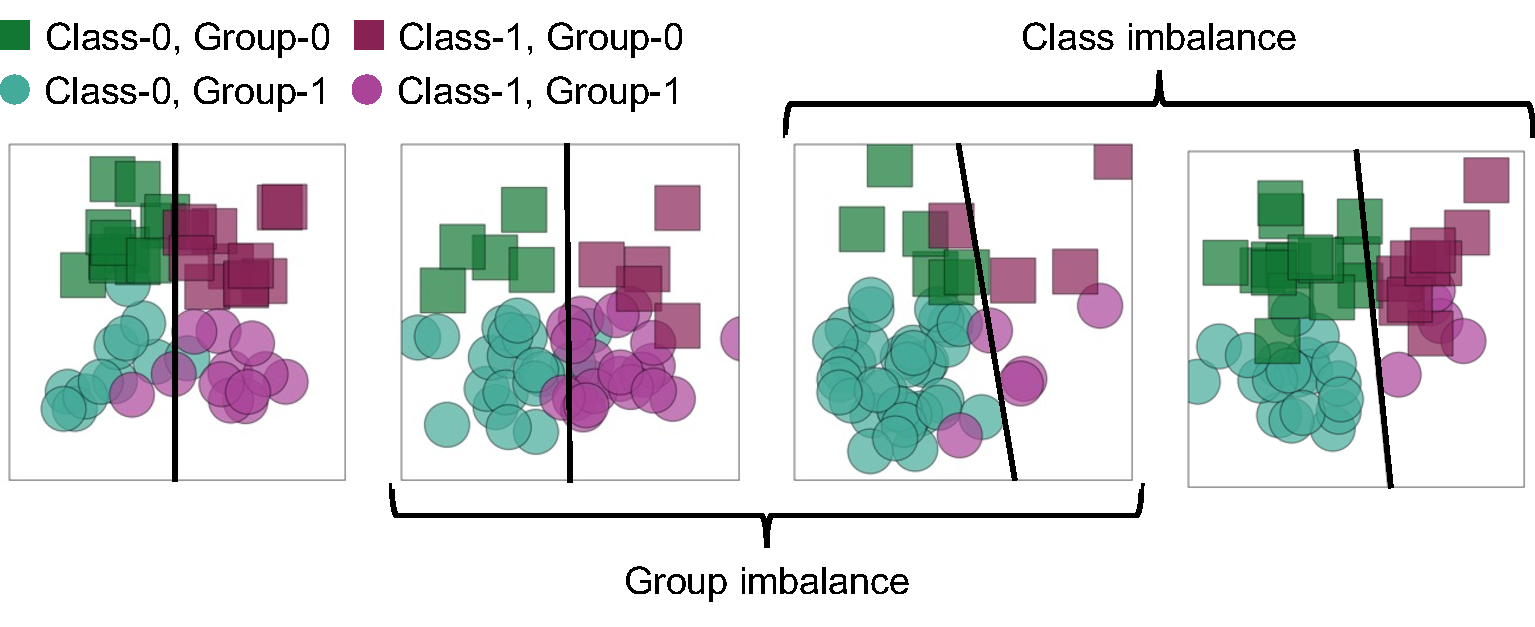
\includegraphics[width=1.0\linewidth]{figures/fairness_toy_exp_2.pdf}
    \caption{\textbf{Influence of the class and group imbalance on classifier during training.} 
    The 2D data are sampled from the normal distributions with four different means and the same covariance. 
    We simulate 4 different experiments with the latent group imbalance (sensitive attributes) by adjusting the number of data in each group.
    The total number of samples is the same.
    We train classifiers for the classes on different imbalance settings and visualize the learned classifiers (bold black lines).
    The fairer the classifiers, the more vertically aligned.
    % When both classes and groups are imbalanced, it yields the most unfair classifier. 
    The classifier trained on the class imbalance is more unfair than the one on the group imbalance.
    % The experiment setting details can be found in the supplementary material.
    }
    \label{fig:fair_toy}
\end{figure}



\begin{table}[]
    \centering
    \begin{subtable}{0.95\linewidth}
        \centering
        \resizebox{\linewidth}{!}{
            \begin{tabular}{lcccc}
            \toprule
            \textbf{Method} & \textbf{Accuracy} & \textbf{DP} & \textbf{ED} & \textbf{EO}\\
            \midrule
            \multicolumn{5}{c}{ResNet18} \\
            \midrule
            % ERM & 93.9 & 0.08174 & 0.0632 & 0.0779\\
            % SYNAuG & 94.0 & 0.06995 & 0.0563 & 0.06825\\
            ERM & 93.9 & 0.0817 & 0.0632 & 0.0779\\
            SYNAuG & \textbf{94.1} & \textbf{0.060} & \textbf{0.0462} & \textbf{0.0434}\\
            \midrule
            \multicolumn{5}{c}{ResNet50} \\
            \midrule
            % ERM & 94.0 & 0.07272 & 0.0585 & 0.07269\\
            % SYNAuG & \textbf{94.1} & \textbf{0.06138} & \textbf{0.04723} & \textbf{0.05885}\\
            ERM & 94.0 & 0.07272 & 0.0585 & 0.07269\\
            SYNAuG & \textbf{94.4} & \textbf{0.05432} & \textbf{0.03936} & \textbf{0.05472}\\
            \bottomrule
           \end{tabular}
        }
    \caption{\textbf{Fairness performance.}}
    \vspace{2mm}
    \label{tab:fairness_1}
    \end{subtable}

    \begin{subtable}{0.95\linewidth}
        \centering
        \resizebox{\linewidth}{!}{
            \begin{tabular}{lcccc}
            \toprule
            \textbf{Method} & \textbf{Accuracy} & \textbf{DP} & \textbf{ED} & \textbf{EO}\\
            \midrule
            ERM & 93.9 & 0.08174 & 0.0632 & 0.0779\\
            + Group-DRO & 93.9 & 0.07266 & 0.05819 & 0.06954\\
            + RS & 93.8 & \textbf{0.0636} & \textbf{0.04663} & \textbf{0.05808} \\
            \midrule
            SYNAuG & \textbf{94.0} & 0.06995 & 0.0563 & 0.06825\\
            + Group-DRO & 93.9 & 0.0711 & 0.05433 & 0.07045\\
            + RS & 93.6 & 0.06786  & 0.06439 & 0.0812 \\
            \bottomrule
           \end{tabular}
        }
       \caption{\textbf{Ablation with other algorithms}}
       \vspace{2mm}
       \label{tab:fairness_2}
   \end{subtable}

    \begin{subtable}{0.95\linewidth}
        \centering
        \resizebox{\linewidth}{!}{
            \begin{tabular}{lcccc}
            \toprule
            \textbf{Method} & \textbf{Accuracy} & \textbf{DP} & \textbf{ED} & \textbf{EO}\\
            \midrule
            ERM & 93.9 & 0.08174 & 0.0632 & 0.0779\\
            + Mixup & 93.9 & 0.07266 & 0.05819 & 0.06954\\
            + CutMix & 94.7 & 0.08265 & 0.06245 & 0.08333\\
            \midrule
            SYNAuG& 94.0 & 0.06995 & 0.0563 & 0.06825\\
            + Mixup & 94.2 & \textbf{0.064} & \textbf{0.03793} & \textbf{0.04658}\\
            + CutMix & \textbf{94.9} & 0.0743 & 0.04745 & 0.06319\\
            \bottomrule
           \end{tabular}
        }
       \caption{\textbf{Augmentation abalation}}
       \vspace{2mm}
       \label{tab:fairness_3}
   \end{subtable}

    \begin{subtable}{0.95\linewidth}
        \centering
        \resizebox{\linewidth}{!}{
            \begin{tabular}{lcccc}
            \toprule
            \textbf{Method} & \textbf{Accuracy} & \textbf{DP} & \textbf{ED} & \textbf{EO}\\
            \midrule
            SYNAuG$^*$ & \textbf{94.0} & 0.07342 & 0.05805 & 0.07253\\ 
            SYNAuG & \textbf{94.0} & \textbf{0.06995} & \textbf{0.0563} & \textbf{0.06825}\\ 
            \bottomrule
            \addlinespace[0.2mm]
            \multicolumn{5}{l}{*Not use the sensitivity attribute}
           \end{tabular}
        }
       \caption{\textbf{Sensitivity abalation}}
       \label{tab:fairness_4}
   \end{subtable}
   
   \caption{\textbf{Fairness performance.} 
   (a) accuracy and model fairness results of our SYNAuG, 
   (b) compatibility with other fairness algorithms, Group-DRO and Re-Sampling (RS), 
   (c) ablation study with data augmentation, Mixup and Cuxmix, 
   and (d) ablation study using the prior about sensitive attribute. \textbf{Bold} means the highest accuracy and the best fairness performance in a table. 
   Higher is better in accuracy, and lower is better in fairness metrics.}
   \label{tab:temps}
\end{table}

Group imbalance stands for the data imbalance between groups, such as ethnicity. 
We empirically observe that the group imbalance with the class imbalance amplifies 
% yields
unfair classifiers, as shown in \Fref{fig:fair_toy}.
The class imbalance affects the unfair classifier more than the group imbalance.
Both class and group imbalance contribute to the unfair classifier.

Model fairness, one of the problems caused by group imbalance, is essential to prevent unexpected social confusion.
Fairness metrics have been proposed to measure the fairness performance of models:
Demographic Parity (DP) $=\max_z|P(y_p{=}1|z) {-} P(y_p{=}1)|$ \cite{10.1145/2783258.2783311},
Equal Opportunity (EO) $=\max_{z_i, z_j, y, y_p}|P_{z_i}(y_p|y) {-} P_{z_j}(y_p|y)|$ \cite{hardt2016equality, jung2022learning},
and Equalized Odds (ED) $=\max_{z, y, y_p}|P(y_p|z, y) {-} P(y_p|y)|$ \cite{hardt2016equality}, where $y_p$ is the prediction, $y$ is the class label, and $z$ is the sensitive attribute.
These metrics are based on the difference in the performance of the learned classifiers depending on groups, \ie, the sensitive attributes.
Lower values of fairness metrics indicate that the model is fairer.


% \begin{table*}[t]
%     \begin{subtable}[b]{0.49\linewidth}
%         \centering
%         \resizebox{\linewidth}{!}{
%             \begin{tabular}{lcccc}
%             \toprule
%             Method & Accuracy & DP & ED & EO \\
%             \midrule
%             % ERM & 93.9 & 0.08174 & 0.0632 & 0.0779\\
%             % SYNAuG$^*$ & \textbf{94.0} & 0.07342 & 0.05805 & 0.07253\\ ICCV 
%             % SYNAuG & \textbf{94.0} & \textbf{0.06995} & \textbf{0.0563} & \textbf{0.06825}\\ ICCB
%             ERM & 93.9 & 0.0817 & 0.0632 & 0.0779\\
%             SYNAuG & \textbf{94.1} & \textbf{0.060} & \textbf{0.0462} & \textbf{0.0434}\\
%             \bottomrule
%            \end{tabular}}
%        \caption{\textbf{Balancing with SYNAuG.}}
%        \label{tab:fair_syn}
%     \end{subtable}
%     \hfill
%     \begin{subtable}[b]{0.49\linewidth}
%         \centering
%         \resizebox{\linewidth}{!}{
%             \begin{tabular}{lcccc}
%             \toprule
%             Method & Accuracy & DP & ED & EO\\
%             \midrule
%             ERM & 93.9 & 0.08174 & 0.0632 & 0.0779\\
%             + Groupp-DRO & 93.9 & 0.07266 & 0.05819 & 0.06954\\
%             + RW & 93.8 & 0.0636 & 0.04663 & 0.05808 \\
%             \midrule
%             SYNAuG & \textbf{94.0} & \textbf{0.06995} & 0.0563 & \textbf{0.06825}\\
%             + Group-DRO & 93.9 & 0.0711 & \textbf{0.05433} & 0.07045\\
%             + RW & 93.6 & 0.06786  & 0.06439 & 0.0812 \\
%             \bottomrule
%            \end{tabular}
%         }
%        \caption{\textbf{Algorithm generalization}}
%        \label{tab:week2}
%    \end{subtable}
   
%     \begin{subtable}[b]{0.49\linewidth}
%         \centering
%         \resizebox{\linewidth}{!}{
%             \begin{tabular}{lcccc}
%             \toprule
%             Method & Accuracy & DP & ED & EO\\
%             \midrule
%             ERM & 93.9 & 0.08174 & 0.0632 & 0.0779\\
%             + Mixup & 93.9 & 0.07266 & 0.05819 & 0.06954\\
%             + CutMix & 94.7 & 0.08265 & 0.06245 & 0.08333\\
%             \midrule
%             SYNAuG& 94.0 & 0.06995 & 0.0563 & 0.06825\\
%             + Mixup & 94.2 & \textbf{0.064} & \textbf{0.03793} & \textbf{0.04658}\\
%             + CutMix & \textbf{94.9} & 0.0743 & 0.04745 & 0.06319\\
%             \bottomrule
%            \end{tabular}
%         }
%        \caption{\textbf{Augmentation generalization}}
%        \label{tab:week2}
%    \end{subtable}
%    \hfill
%    \begin{subtable}[b]{0.49\linewidth}
%         \centering
%         \resizebox{\linewidth}{!}{
%             \begin{tabular}{lcccc}
%             \toprule
%             Method & Accuracy & DP & ED & EO\\
%             \midrule
%             \multicolumn{5}{c}{ResNet18} \\
%             \midrule
%             % ERM & 93.9 & 0.08174 & 0.0632 & 0.0779\\
%             % SYNAuG & 94.0 & 0.06995 & 0.0563 & 0.06825\\
%             ERM & 93.9 & 0.0817 & 0.0632 & 0.0779\\
%             SYNAuG & \textbf{94.1} & \textbf{0.060} & \textbf{0.0462} & \textbf{0.0434}\\
%             \midrule
%             \multicolumn{5}{c}{ResNet50} \\
%             \midrule
%             % ERM & 94.0 & 0.07272 & 0.0585 & 0.07269\\
%             % SYNAuG & \textbf{94.1} & \textbf{0.06138} & \textbf{0.04723} & \textbf{0.05885}\\
%             ERM & 94.0 & 0.07272 & 0.0585 & 0.07269\\
%             SYNAuG & \textbf{94.4} & \textbf{0.05432} & \textbf{0.03936} & \textbf{0.05472}\\
%             \bottomrule
%            \end{tabular}
%         }
%        \caption{\textbf{Architecture generalization.}}
%        \label{tab:week2}
%    \end{subtable}
     
%      \caption{\textbf{Fairness performance.} (a) shows the result of our SYNAuG, (b) the experiments with Group-DRO, (c) the experiments with data augmentation, Mixup and Cuxmix, and (d) experiments with deeper architecture, ResNet50. \textbf{Bold} means the highest accuracy and the best fairness performance in a table. Higher is better in accuracy, and lower is better in fairness metrics.}
%      \label{tab:temps}
%      \vspace{-5mm}
% \end{table*}

\paragraph{Experiments on UTKFace.}
We employ UTKFace~\cite{zhifei2017cvpr} composed of 23,708 images with age, gender, and race labels.
We use race annotation as a sensitive attribute (group label) and gender as the class label.
For SYNAuG, we augment the data to mitigate the class imbalance across the sensitive attribute;
the female and male ratio of each sensitive attribute becomes equal.
%We evaluate the accuracy and fairness metric from the model at the last epoch.
% 바로 뒤에는 fairness metrics 로 쓰셔서 혹시 몰라 적어놓겠습니다.
We evaluate the accuracy and fairness metrics from the model at the last epoch.
Firstly, we validate the effectiveness of SYNAuG in \Tref{tab:fairness_1}.
The result shows that SYNAuG outperforms ERM in accuracy and fairness metrics on both ResNet18 and ResNet50.

\paragraph{Ablation with other algorithms.} 
%In \Tref{tab:fairness_2}, we experiment with the algorithm explaining the sensitive attributes, Group-DRO~\cite{sagawa2019distributionally} and Re-Sampling (RS).
% 바로 위와 같은 이유로 달아 놓겠습니다.
In \Tref{tab:fairness_2}, we evaluate the performance of the two algorithms Group-DRO~\cite{sagawa2019distributionally} and Re-Sampling (RS).
Note that we do not apply Mixup and fine-tuning in this experiment.
Group-DRO and RS improve the fairness metrics of ERM at the same time.
SYNAuG without Group-DRO outperforms the accuracy and two fairness metrics, ED and EO, compared to Group-DRO.
Developing a fairness algorithm with synthetic data might be a promising direction toward a fair model.

\paragraph{Augmentation ablation.} 
In \Tref{tab:fairness_3}, we compare the effect of data augmentations, Mixup~\cite{zhang2017mixup} and CutMix~\cite{yun2019cutmix}.
In this ablation study, we do not apply fine-tuning for clear comparison.
Both augmentations improve the accuracy of ERM; Mixup also works 
% does
in the fairness metrics.
Compared to ERM with Mixup, SYNAuG shows higher accuracy and better fairness metrics.
% EO metric, but underperforms in the other two metrics.
SYNAuG with Mixup outperforms more in accuracy and fairness metrics compared to ERM with Mixup.


\paragraph{No prior of sensitive attribute.}
Labeling sensitive attributes might be expensive.
In this ablation study, we augment the synthetic data to mitigate the class imbalance regardless of sensitive attributes.
We denote this setting as SYNAuG$^*$.
As shown in \Tref{tab:fairness_4}, SYNAuG$^*$ shows better fairness metrics compared to ERM.
However, exploiting the knowledge of sensitive attributes is more effective.

\paragraph{Summary.} 
Class imbalance in fairness can easily cause an unfair model.
This motivates us to balance the class imbalance using synthetic data before tackling fairness directly.
We observe that the synthetic data improves both model accuracy and fairness simultaneously.
The experimental results also demonstrate that SYNAuG is compatible with other training algorithms, data augmentation, and network architecture.




\begin{table*}[t]
\centering
\resizebox{0.65\linewidth}{!}{
    \begin{tabular}{@{}lcccccc}
        \toprule
        \multirow{2}[2]{*}{\textbf{{Method}}} & \multicolumn{4}{c}{\textbf{IF=100}} & \multirow{2}[2]{*}{\textbf{{50}}} & \multirow{2}[2]{*}{\textbf{{10}}} \\
        \cmidrule{2-5}
        & \textbf{Many} & \textbf{Medium} & \textbf{Few} & \textbf{All} & & \\
        \midrule
        CE~\cite{cui2019class}                         & 68.31 & 36.88 & 4.87 & 37.96 & 43.54 & 59.50 \\
        \cmidrule{1-7}
        SSD~\cite{li2021self}                          & - & - & - & 46.0 & 50.5 & 62.3 \\
        PaCo~\cite{cui2021parametric}                  & - & - & - & 52.0 & 56.0 & 64.2 \\
        RISDA~\cite{chen2022imagine}                   & - & - & - & 50.16 & 53.84 & 62.38 \\
        CE + CMO~\cite{park2022majority}               & 70.4 & 42.5 & 14.4 & 43.9 & 48.3 & 59.5 \\
        LDAM + CMO~\cite{park2022majority}             & 61.5 & 48.6 & 28.8 & 47.2 & 51.7 & 58.4 \\
        RIDE (3 experts) + CMO~\cite{park2022majority} & - & - & - & 50.0 & 53.0 & 60.2 \\
        Weight Balancing~\cite{alshammari2022long}     & 72.60 & 51.86 & 32.63 & 53.35 & 57.71 & 68.67 \\
        \cmidrule{1-7}
        % Web crawled images                        & 72.71 & 51.21 & 36.13 & 54.06 & 56.40 & 63.86 \\
        % \cmidrule{1-7}
        % Intra-class Image Translation             & 71.86 & 45.88 & 22.97 & 47.87 & 53.33 & 64.95 \\
        % Inter-class Image Translation             & 73.49 & 45.77 & 19.00 & 47.17 & 51.33 & 64.11 \\
        % Class Distribution Fitting                & \textbf{74.83} & 50.79 & 26.03 & 51.53 & 55.60 & 65.60 \\
        % \cmidrule{1-7}
        SYNAuG                                    & \textbf{74.06} & \textbf{56.63} & \textbf{42.83} & \textbf{58.59} & \textbf{61.36} & \textbf{69.01} \\
        % SYNAuG                                         & 74.66 & 52.21 & 27.52 & 52.41 & 56.99 & 66.34 \\
        % SYNAuGAttr                                     & 75.23 & 52.15 & 30.58 & 53.54 & 57.09 & 66.66 \\
        % SYNAuG + Mixup                                 & 75.37 & 54.24 & 32.16 & 54.79 & 57.55 & 66.66 \\
        % SYNAuGAttr + Mixup                             & 74.97 & 53.77 & 35.26 & 55.45 & 58.69 & 66.84 \\
        % SYNAuGAttr + classifier re-training            & 74.83 & 52.57 & 33.13 & 54.53 & 57.93 & 66.80 \\
        % SYNAuGAttr + classifier fine-tuning            & 74.43 & 53.26 & 32.97 & 54.58 & 58.26 & 67.24 \\
        % SYNAuGAttr + Mixup + classifier re-training    & 73.97 & 56.26 & 39.10 & 57.31 & 60.34 & 67.90 \\
        % SYNAuGAttr + Mixup + classifier fine-tuning    & 74.06 & 56.63 & 42.83 & 58.59 & 61.36 & 69.01 \\
        \bottomrule 
    \end{tabular}
    }
    \caption{\textbf{Long-tailed recognition performance on CIFAR100-LT.}
    We compare our SYNAuG with recent works in long-tailed recognition.
    We report the Top-1 accuracy (\%) with different imbalance factors, \ie, IF=\{100, 50, 10\}.
    % \textbf{Bold} stands for the highest accuracy in each IF or class.
    }
    \label{tab:cifar100_lt}
\end{table*}

\begin{table}[t]
\centering
\resizebox{1.0\linewidth}{!}{
    \begin{tabular}{@{}lcccc}
        \toprule
        \multirow{2}[2]{*}{\textbf{{Method}}} & \multirow{2}[2]{*}{\textbf{\makecell{Additional\\Data Type}}}& \multicolumn{3}{c}{\textbf{IF}} \\
        \cmidrule{3-5}
        & & \textbf{100} & \textbf{50} & \textbf{10}\\
        \midrule
        CE~\cite{cui2019class} & N/A & 37.96 & 43.54 & 59.50 \\                        
        % & 68.31 & 36.88 & 4.87 & 37.96 & 43.54 & 59.50 \\
        \cmidrule{1-5}
        Web crawled images    & Real & 54.06 & 56.40 & 63.86 \\
        % & 72.71 & 51.21 & 36.13 & 54.06 & 56.40 & 63.86 \\
        \cmidrule{1-5}
        Intra-class Image Translation & Syn. & 47.87 & 53.33 & 64.95 \\
        % & 71.86 & 45.88 & 22.97 & 47.87 & 53.33 & 64.95 \\
        Inter-class Image Translation & Syn. & 47.17 & 51.33 & 64.11 \\
        % & 73.49 & 45.77 & 19.00 & 47.17 & 51.33 & 64.11 \\
        Class Distribution Fitting     & Syn. & 51.53 & 55.60 & 65.60 \\
        % & \textbf{74.83} & 50.79 & 26.03 & 51.53 & 55.60 & 65.60 \\
        \cmidrule{1-5}
        SYNAuG                          & Syn. & \textbf{58.59} & \textbf{61.36} & \textbf{69.01} \\
        % & 74.06 & \textbf{56.63} & \textbf{42.83} & \textbf{58.59} & \textbf{61.36} & \textbf{69.01} \\
        \bottomrule 
    \end{tabular}
    }
    \caption{\textbf{Comparison with the baselines.}
    We use CIFAR100-LT.
    The second column denotes the data type used in uniformization.
    % with different imbalance factors, \ie, IF=\{100, 50, 10\}.
    % \textbf{Bold} stands for the highest accuracy in each IF or class.
    }
    \label{tab:cifar100_lt_baseline}
\end{table}


\begin{table}[t]
\centering
\resizebox{1.0\linewidth}{!}{
    \begin{tabular}{cccccccc}
        \toprule
        \multirow{2}[2]{*}{} & \multirow{2}[2]{*}{\textbf{Modifier}} & \multirow{2}[2]{*}{\textbf{Mixup}} & \multirow{2}[2]{*}{\textbf{Re-train}} & \multirow{2}[2]{*}{\textbf{Finetune}} & \multicolumn{3}{c}{\textbf{IF}} \\ \cmidrule{6-8}
        & & & & & \textbf{100} & \textbf{{50}} & \textbf{{10}} \\
        \midrule
        (a) & & & & & 52.41 & 56.99 & 66.34 \\
        (b) & \checkmark & & & & 53.54 & 57.09 & 66.66 \\
        % (c) & & \checkmark &  & 54.79 & 57.55 & 66.66 \\
        (c) & \checkmark & \checkmark & & & 55.45 & 58.69 & 66.84 \\
        (d) & \checkmark & \checkmark & \checkmark & & 57.31 & 60.34 & 67.90 \\
        (e) & \checkmark & \checkmark & & \checkmark & \textbf{58.59} & \textbf{61.36} & \textbf{69.01} \\
        \bottomrule 
    \end{tabular}
    }
    \caption{\textbf{Ablation study of SYNAuG.} 
    We use CIFAR100-LT.
    Each component, Modifier, Mixup, Re-train, and Finetune, means we use the class-related modifiers in the prompt, use Mixup augmentation during training, and re-train or finetune the last layer after training, respectively.
    (e) stands for our SYNAuG.
    }
    \label{tab:ablation}
\end{table}



\paragraph{Experimental setting.}
We employ two long-tail datasets: CIFAR100-LT~\cite{cao2019learning} and ImageNet100-LT~\cite{jiang2021self}.
CIFAR100-LT and ImageNet100-LT have train sets that are artificially curated to make class imbalance from the original datasets, CIFAR100~\cite{krizhevsky2009learning} and ImageNet100~\cite{tian2020contrastive}.
The test sets for them are the same as the original one.
The classes in the long-tailed datasets are divided into three groups: Many-shot (more than 100 samples), Medium-shot (20-100 samples), and Few-shot (less than 20 samples).
For CIFAR100-LT, the imbalance factor (IF) can be controlled by computing the ratio of samples in the head to tail class, $N_1/N_K$, where $N_k=\left| \mathcal{D}_k\right|$, and $\mathcal{D}_k$ is the set of samples belonging to the class $k\in\{1,\cdots,K\}$.
As the IF value increases, the skewness of the training data becomes more severe, which makes it more challenging.
%When the IF value is large, the skewness of the training data is more severe, which has fewer samples and is more challenging.
We evaluate under the standard IFs of 100, 50, and 10, following~\cite{alshammari2022long}.
We use ResNet32 for CIFAR100-LT and ResNet50 for ImageNet100-LT.
Further details can be found in the supplementary material.


\paragraph{Competing methods and baselines.}
We compare with recent prior arts: SSD~\cite{li2021self} and PaCo~\cite{cui2021parametric} for self-supervised learning, RISDA~\cite{chen2022imagine} and CMO~\cite{park2022majority} for data augmentation, and Weight Balancing~\cite{alshammari2022long} for the rebalance classifier.
They are state-of-the-art in each perspective and propose methods only using 
% limited to 
the original long-tailed data without external data sources.
% As a strong baseline in terms of data supplement perspective, we collect the data from the internet to populate the insufficient samples, named as WebAug.

We present other 
% baselines by using 
variants of generation methods as baselines:
1) Motivated by the recent work~\cite{he2022synthetic} using the few-shot original samples as guidance during the generation process, we first introduce
% For 
\emph{Intra-class Image Translation}, where we use the original samples from the original training data as a class-wise guidance image for generation,
% It is motivated by the recent work~\cite{he2022synthetic} using the few-shot original samples as guidance during the generation process.
2) Inspired by the M2m~\cite{kim2020m2m} translating an image of the major class to the minor class for leveraging the diversity of the majority information, we introduce
% For 
\emph{Inter-class Image Translation}, where we utilize random samples in the dataset as guidance regardless of the class,
% It is inspired by the M2m~\cite{kim2020m2m} translating an image of the major class to the minor class for leveraging the diversity of the majority information.
3) As an advanced version motivated by DreamBooth~\cite{ruiz2022dreambooth}, we fine-tune the diffusion model with the samples in each class to model the class-wise distribution, named \emph{Class Distribution Fitting},
% ,\footnote{During fine-tuning, we add infrequently used text fragment, such as ``pqk'', as a class token before the target class word in the prompt.
% After fine-tuning the generative model, the added text fragment would become a token that includes the class information.
% The fine-tuned generative model generates synthetic samples for populating the training distribution.}
and 4) As a strong baseline, we collect the real data from the internet instead of generating synthetic images, \ie, \emph{Web crawled images}.
Details are in the supplementary material.


\paragraph{Comparison results.}
We compare SYNAuG with the prior arts in \Tref{tab:cifar100_lt}.
Compared to the CE method~\cite{cui2019class} trained with the Cross Entropy loss on the original data, we achieve large improvements when exploiting the generated samples regardless of the skewness of the training data.
Our method also outperforms 
% shows outperformed performance compared to 
most of the competing methods.
This is stunning results in that it
% The results 
suggests 
% demonstrates
that relieving the imbalance from the data point of view is simple but more effective than the conventional complex algorithmic methods.


In \Tref{tab:cifar100_lt_baseline}, we compare our method with our proposed baselines.
Compared to the case that uses real-world web data\footnote{We collected image from Google image search. Google image search returns images very favorable to DNNs, because Google has used CNN-based image search since March 2013~\cite{chen2015webly}. Thus, using web data is analogous to the distillation of a Google internal model, \ie, very strong baseline.}, it shows that the generated images are of sufficient quality to mitigate the class imbalance problem.
Also, we evaluate additional baselines, which apply the variant methods during the generation process.
% explained in \Sref{sec:2.3} during the generation process.
While they are better than training only with the original long-tailed data (CE method~\cite{cui2019class}), the performance is lower than SYNAuG.
The results imply that the domain gap between the original and synthetic data is hard to narrow during the generation process.
Thus, we propose to leverage 
% using
Mixup during training and fine-tuning the classifier as a more straightforward way.
Note that na\"ively applying Mixup to imbalanced data cases is known to be detrimental~\cite{yebin2023textmania}; thus, we distinctively apply Mixup after uniformizing data distribution which makes a noticeable difference.


\paragraph{Ablation study.}
In \Tref{tab:ablation}, we conduct an ablation study to investigate the influence of each component of our SYNAuG.
When we use modifiers in the prompt, we can get diverse generated samples, which result in the gain between (a) and (b).
We can achieve further improvement by utilizing Mixup (c) to interpolate between original and synthetic data, whereby the domain gap is mitigated by bridging two different domain data.
% the mixed-up data acts as a bridge between the two groups, significantly improving performance.
%When we utilize Mixup (c) for interpolating between original and synthetic data, we can achieve further improvement.
%The mixed-up with original data serves as a bridge between the two groups, affecting largely performance improvement.
Despite the domain Mixup, 
% bridging samples,
the classifier still has room to be more adjusted toward the target data.
To do so, we can re-train (d) or fine-tune (e) the last layer on the uniform distribution data sampling from the original training data, \ie, we set the number of samples in each data class to the smallest number of samples in the original long-tail training data class.
% each data class has the smallest number of samples among the original long-tailed training data classes.
As shown in \Tref{tab:ablation}-(d,e),
% the results, 
we can achieve an additional improvement by adjusting the classifier towards the targeted real data and found that fine-tuning is more effective than re-training.
% \wonseok{and fine-tuning is found to be more effective than re-training.}
%but fine-tuning is more effective than re-training.




\begin{figure}
    \centering
    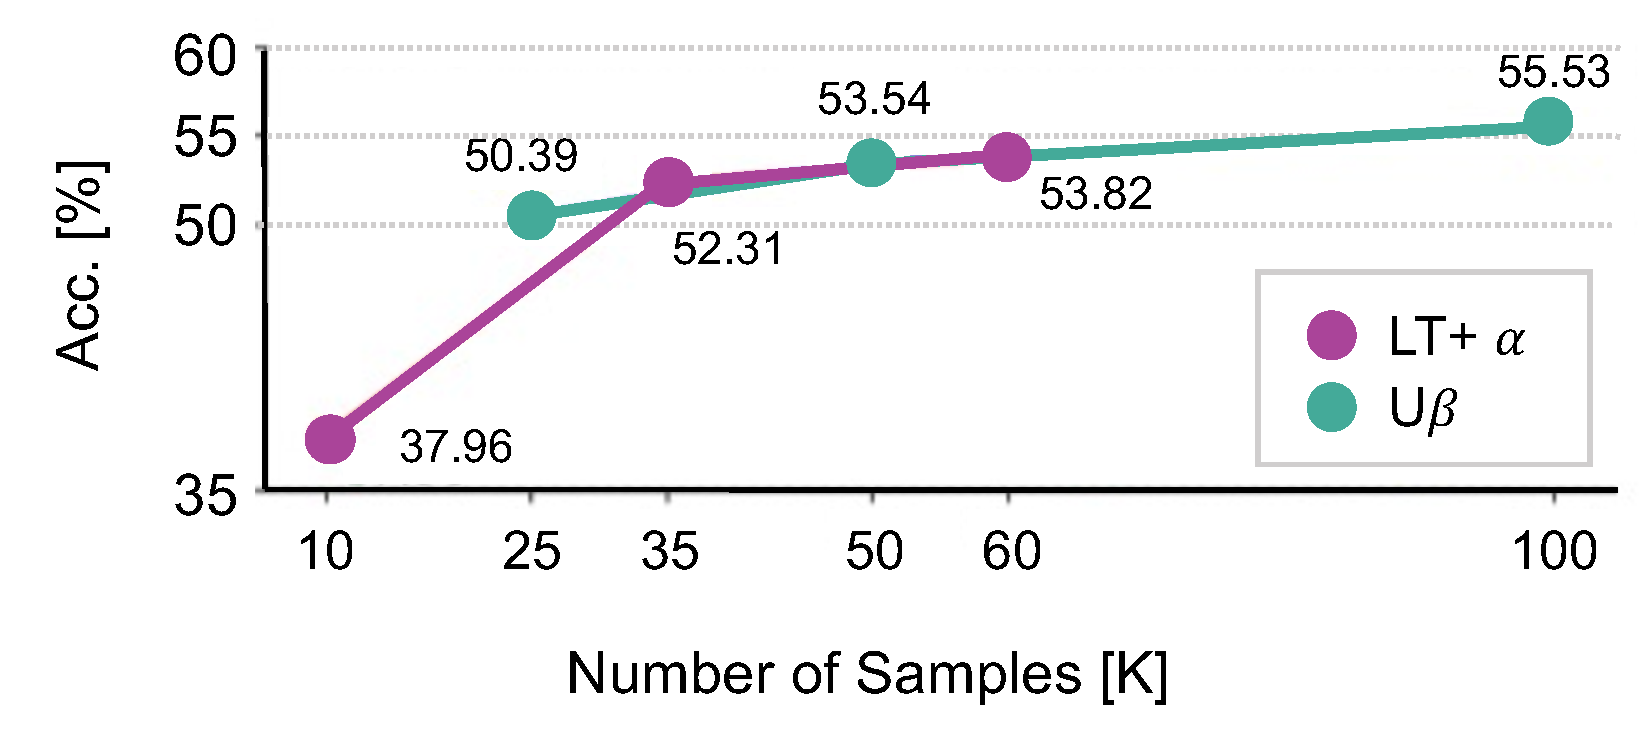
\includegraphics[width=0.95\linewidth]{figures/num_data.pdf}
    \caption{\textbf{Accuracy [\%] (y-axis) vs. number of samples [K] (x-axis).}
    As expected, the performance improves as more synthetic samples are added.
    Additionally, it is improved significantly when the Few class disappears as the number of samples per class increases.}
    \label{fig:alleviate}
\end{figure}



\paragraph{Performance according to the number of synthetic data.}
We explore the performance according to 
% by varying the 
varying number of synthetic data (See \Fref{fig:alleviate}).
We use CIFAR100-LT with the imbalance factor IF=100, \ie, 
% so
the total number of the original samples is 10,847.
%For LT+$\alpha$, we add the synthetic data to all classes equally without care of Many, Medium, and Few classes.
% \wonseok{
For LT+$\alpha$, we uniformly allocate
% incorporate
synthetic data across all classes disregarding the distinction between Many, Medium, and Few classes.
% }
In this case, the absolute difference in sample amount between classes is kept unchanged.
% remains.
%For U$\beta$, we add synthetic data or cut the original samples to be the total number of samples in each class same, \ie, uniformize the data distribution.
% \wonseok{
For U$\beta$, we ensure an equal number of samples in each class by either adding synthetic data or trimming some of the original samples.
% }


% As shown 
In \Fref{fig:alleviate}, the performance is improved as the number of samples increases regardless of the data distribution.
As the quantity of synthetic data increases, accuracies of LT+$\alpha$ and U$\beta$ become quite similar.
%We think that LT+$\alpha$ becomes far from the long-tailed distribution, \ie, the Few class becomes not Few anymore, although the difference in data amount across classes remains in LT+$\alpha$, which reduces the gap between LT+$\alpha$ and U$\beta$.
% 
% \wonseok{
We think that LT+$\alpha$ tends to deviate from the long-tailed distribution as the number
% quantity
of synthetic data increases, \ie, the Few class becomes not Few anymore. Although the disparities 
% variation
in data quantities across classes exist in LT+$\alpha$, this effect diminishes the difference 
% disparity
between LT+$\alpha$ and U$\beta$ with more synthetic data.
% }





\paragraph{Performance according to the quality of synthetic data.}
We evaluate SYNAuG on ImageNet100-LT.
% considering high resolution.
% Since the step value in Stable Diffusion~\cite{rombach2022high} is known to affect the quality of generated images, 
We conduct an ablation study to investigate the impact of data quality of
% different step values
% on
SYNAuG by controlling the diffusion step parameter
% Since the step value in 
of Stable Diffusion~\cite{rombach2022high}, which is known to affect the quality of generated images.
As shown in 
% On the top of
\Fref{fig:imagenet100_lt}-(Top), the generation quality is low when the number of steps is very small, but there is no big difference to the naked eye as it goes up to a certain number.
Figure~\ref{fig:imagenet100_lt}-(Bottom) shows the quantitative results.
% These results lead to quantitative results as well, as shown at the bottom of \Fref{fig:imagenet100_lt}.
Compared to the CE method~\cite{cui2019class} trained on the original long-tailed data, while the accuracy of the Many class is degraded, we achieve large improvement in the Medium, Few, and even All cases
% in all the classes 
regardless of the synthetic image quality.
% Although the accuracy of the Many class is degraded, overall performance, including Medium and Few classes, is drastically improved.
%The results are considerably apart between using synthetic samples with low quality and one with a certain level of quality, but the difference is marginal when the image quality according to the step value exceeds the threshold.
However, there is a certain level of quality that exhibits a surge point in performance.
% The results are 
% considerably different between using synthetic samples with low quality and one with a certain level of quality. 
% However, 
The difference becomes negligible when 
% the image quality according to 
the step value exceeds a certain threshold, \ie, quality.


\begin{figure}[t]
    \begin{subfigure}[c]{0.9\linewidth}
        \centering
        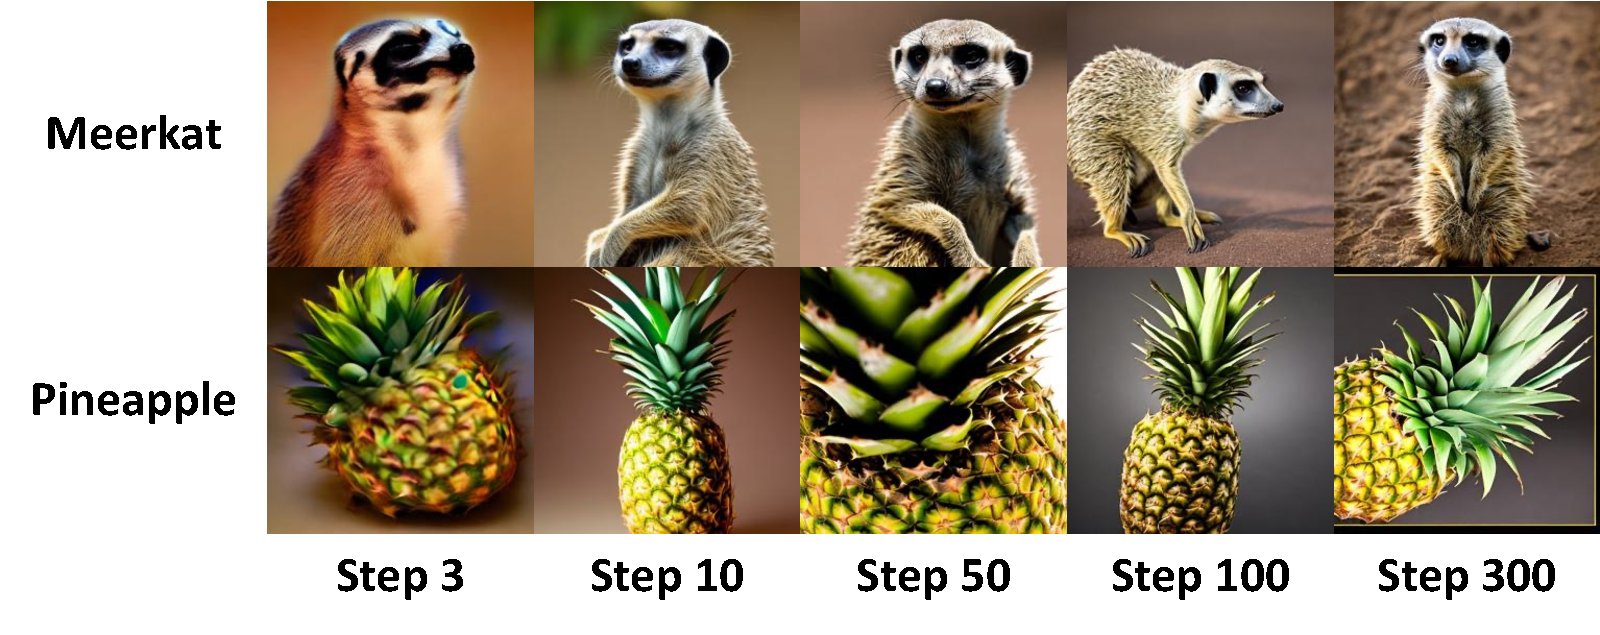
\includegraphics[width=1.0\linewidth]{figures/stepqual_vis.pdf}
    \end{subfigure}
    \centering
    \begin{subtable}[c]{0.9\linewidth}
    \resizebox{1.0\linewidth}{!}{
        \begin{tabular}{@{\,\,\,}lccccc}
            \toprule
            \textbf{Method}  & \textbf{\# step} & \textbf{Many} & \textbf{Medium} & \textbf{Few} & \textbf{All} \\
            \midrule
            CE~\cite{cui2019class}   & & \textbf{61.85} & 15.83 &  0.29 & 32.06 \\
            \cmidrule{1-6}
            \multirow{5}{*}{SYNAuG}
            & 3    & 48.23 & 46.29 & 40.07 & 45.10 \\
            & 10   & 53.89 & \textbf{49.49} & 43.87 & \textbf{49.34} \\
            & 50   & 52.91 & 48.63 & \textbf{45.27} & 49.12 \\
            & 100  & 53.03 & 49.20 & 44.47 & 49.12 \\
            & 300  & 54.11 & 47.71 & 44.73 & 49.06 \\
            \bottomrule 
        \end{tabular}
        }
    \end{subtable}
\caption{\textbf{Ablation study according to sample quality.}
\textbf{(Top)} quality of the generated samples according to the number of steps, \textbf{(Bottom)} long-tailed recognition performance (\%) 
% We report the Top-1 accuracy (\%) 
according to the different times of steps for generating synthetic data, which affects sample quality.
We use ImageNet100-LT with ResNet50.
}
\label{fig:imagenet100_lt}
\end{figure}









A class may include dominant patterns, \ie, spurious correlations.
For example, waterbirds are usually on water rather than land.
It leads DNNs to rely heavily on these spurious features rather than reasoning; thereby, DNNs classify water images as waterbirds regardless of the existence of waterbirds.
This spurious correlation is also caused by data imbalance because fewer waterbirds are located on land.
While spurious correlation occurs naturally, we can mitigate their impact by resolving data imbalance
% generating samples
similar to model fairness.
% long-tailed distribution.
% not to be correlated with spurious features.
We demonstrate whether SYNAuG can mitigate the data imbalance problem of spurious correlations.

% % which can drift the model to cause bias or misconception, \ie, spurious correlations.
% % DNNs heavily rely on these spurious features rather than reasoning, because these features are easy to learn.
% For example, DNNs can classify the empty road image as the models are trained with lots of car images on a road that usually takes a much larger area than that of cars.
% % spurious corr하고 imbalance하고 연관
% Although spurious correlations caaturally, we can mitigate their impact by generating samples in rare classes that are not correlated with the sensitive attributes.
% % to generate rare samples using diffusion models.
% We demonstrate whether SYNAuG can mitigate the data imbalance problem, which causes spurious correlations.


\begin{table}
    \centering
        \resizebox{0.9\linewidth}{!}{
            \begin{tabular}{lcc}
            \toprule
            \multirow{2}[2]{*}{\textbf{Method}} & \multicolumn{2}{c}{\textbf{Waterbirds}}\\
            \cmidrule{2-3}
            & \textbf{Worst} & \textbf{Mean}\\
            \midrule
            ERM & 72.6 & 97.3\\
            JTT$_\texttt{ ICML'21}$~\cite{liu2021just} & 86.7 & 93.3 \\
            Group-DRO$_\texttt{ ICLR'20}$~\cite{sagawa2019distributionally} & 91.4 & 93.5\\
            SUBG$_\texttt{ ICML'20}$~\cite{sagawa2020investigation} & 89.1$_{\pm 1.1}$ & -\\
            SSA$_\texttt{ ICLR'22}$~\cite{nam2022spread} & 89.0$_{\pm 0.55}$ & 92.2$_{\pm 0.87}$\\
            \midrule
            BaseModel & 73.7$_{\pm 3.04}$ & 90.4$_{\pm 0.21}$\\
            % BaseModel$_{\text{web}}$ & 80.1$_{\pm 1.95}$ & 94.3$_{\pm 0.38}$\\
            SYNAuG & 79.9$_{\pm 2.22}$ & 91.52$_{\pm 0.98}$\\
            \midrule
            % DFR$^{\text{Tr}}_{\text{Tr}}$$_\texttt{ ICLR'23}$~\cite{kirichenko2023last} & 89.2$_{\pm 1.91}$ & 94.2$_{\pm 0.74}$\\
            % % DFR$^{\text{Tr-web}}_{\text{Tr}}$ & 92.8$_{\pm 1.13}$ & 96.0$_{\pm 0.55}$\\
            % SYNAuG & 90.3$_{\pm 0.81}$ & 93.7$_{\pm 0.24}$\\
            % SYNAuG & 79.8$_{\pm }$ & 92.4$_{\pm }$\\
            % \midrule
            DFR$^{\text{Tr}}_{\text{Val}}$$_\texttt{ ICLR'23}$~\cite{kirichenko2023last} & 91.2$_{\pm 1.92}$ & 93.1$_{\pm 0.91}$\\
            % DFR$^{\text{Tr-web}}_{\text{Val}}$ & 93.9$_{\pm 0.60}$ & 95.4$_{\pm 0.40}$\\
            SYNAuG (re-train) & 92.9$_{\pm 0.45}$ & 93.6$_{\pm 0.35}$\\
            SYNAuG (fine-tuning) & 93.2$_{\pm 0.42}$ & 94.8$_{\pm 0.11}$\\
            \bottomrule
           \end{tabular}}
       \caption{\textbf{Robustness to spurious correlation on Waterbirds.} 
       SYNAuG outperforms DFR consistently in worst-group accuracy.}\vspace{4mm}
       \label{tab:robustness}
\end{table}

\paragraph{Experiments.} 
We use Waterbirds dataset~\cite{sagawa2019distributionally}, which is a synthetic dataset created by combining images of birds from the CUB dataset~\cite{WelinderEtal2010} with backgrounds.
%The seabirds and waterfowl are grouped in a waterbird, and the other birds in a landbird.
The birds are grouped into two categories: waterbirds, which include seabirds and waterfowl, and landbirds.
Land and water background are spurious features.
Let $G_{\text{background}}^{\text{class}}$ be the class with the background, \eg, $G_{\text{water}}^{\text{landbird}}$ is the landbird with water background.
% where the class is waterbirds or landbirds, and the background is land or water.
% Let $G_1, G_2, G_3$, and $G_4$ be landbird with land background, landbird with water background, waterbird on land background, and waterbird with water background, respectively.
In the Waterbirds dataset, $G_{\text{land}}^{\text{landbird}}$ has more samples than $G_{\text{water}}^{\text{landbird}}$, and $G_{\text{water}}^{\text{waterbird}}$ has more samples than $G_{\text{land}}^{\text{waterbird}}$.
We generate the samples to match the number of samples such as $|G_{\text{land}}^{\text{landbird}}| = |G_{\text{water}}^{\text{landbird}}|$ and $|G_{\text{water}}^{\text{waterbird}}| = |G_{\text{land}}^{\text{waterbird}}|$.
% $G_1$ and $G_2$, and $G_3$ and $G_4$.
% Following Sagawa~\etal\cite{sagawa2019distributionally}, we evaluate algorithms using the minimum group accuracy and the average (in-distribution) accuracy, denoted as Worst and Mean, respectively.
We report the result over 5 independent runs using the code from DFR~\cite{kirichenko2023last}.
We reproduce the BaseModel and DFR and report the performance at the last epoch\footnote{\url{https://github.com/PolinaKirichenko/deep_feature_reweighting}}.

In \Tref{tab:robustness}, our SYNAuG generates samples not to be correlated with spurious features, which
improves the performance in BaseModel both on worst and mean accuracies.
When applying DFR, the synthetic data can increase the worst and mean accuracy consistently.
% In addition, w
We also observe that fine-tuning is more effective 
% shows better performance
compared to re-train, which is consistent with \Tref{tab:ablation}.
% It indicates 
The overall results demonstrate that the synthetic data from the generative model can be exploited to mitigate the spurious correlation.



